\documentclass[twoside]{book}

% Packages required by doxygen
\usepackage{fixltx2e}
\usepackage{calc}
\usepackage{doxygen}
\usepackage[export]{adjustbox} % also loads graphicx
\usepackage{graphicx}
\usepackage[utf8]{inputenc}
\usepackage{makeidx}
\usepackage{multicol}
\usepackage{multirow}
\PassOptionsToPackage{warn}{textcomp}
\usepackage{textcomp}
\usepackage[nointegrals]{wasysym}
\usepackage[table]{xcolor}

% Font selection
\usepackage[T1]{fontenc}
\usepackage[scaled=.90]{helvet}
\usepackage{courier}
\usepackage{amssymb}
\usepackage{sectsty}
\renewcommand{\familydefault}{\sfdefault}
\allsectionsfont{%
  \fontseries{bc}\selectfont%
  \color{darkgray}%
}
\renewcommand{\DoxyLabelFont}{%
  \fontseries{bc}\selectfont%
  \color{darkgray}%
}
\newcommand{\+}{\discretionary{\mbox{\scriptsize$\hookleftarrow$}}{}{}}

% Page & text layout
\usepackage{geometry}
\geometry{%
  a4paper,%
  top=2.5cm,%
  bottom=2.5cm,%
  left=2.5cm,%
  right=2.5cm%
}
\tolerance=750
\hfuzz=15pt
\hbadness=750
\setlength{\emergencystretch}{15pt}
\setlength{\parindent}{0cm}
\setlength{\parskip}{3ex plus 2ex minus 2ex}
\makeatletter
\renewcommand{\paragraph}{%
  \@startsection{paragraph}{4}{0ex}{-1.0ex}{1.0ex}{%
    \normalfont\normalsize\bfseries\SS@parafont%
  }%
}
\renewcommand{\subparagraph}{%
  \@startsection{subparagraph}{5}{0ex}{-1.0ex}{1.0ex}{%
    \normalfont\normalsize\bfseries\SS@subparafont%
  }%
}
\makeatother

% Headers & footers
\usepackage{fancyhdr}
\pagestyle{fancyplain}
\fancyhead[LE]{\fancyplain{}{\bfseries\thepage}}
\fancyhead[CE]{\fancyplain{}{}}
\fancyhead[RE]{\fancyplain{}{\bfseries\leftmark}}
\fancyhead[LO]{\fancyplain{}{\bfseries\rightmark}}
\fancyhead[CO]{\fancyplain{}{}}
\fancyhead[RO]{\fancyplain{}{\bfseries\thepage}}
\fancyfoot[LE]{\fancyplain{}{}}
\fancyfoot[CE]{\fancyplain{}{}}
\fancyfoot[RE]{\fancyplain{}{\bfseries\scriptsize Generated by Doxygen }}
\fancyfoot[LO]{\fancyplain{}{\bfseries\scriptsize Generated by Doxygen }}
\fancyfoot[CO]{\fancyplain{}{}}
\fancyfoot[RO]{\fancyplain{}{}}
\renewcommand{\footrulewidth}{0.4pt}
\renewcommand{\chaptermark}[1]{%
  \markboth{#1}{}%
}
\renewcommand{\sectionmark}[1]{%
  \markright{\thesection\ #1}%
}

% Indices & bibliography
\usepackage{natbib}
\usepackage[titles]{tocloft}
\setcounter{tocdepth}{3}
\setcounter{secnumdepth}{5}
\makeindex

% Hyperlinks (required, but should be loaded last)
\usepackage{ifpdf}
\ifpdf
  \usepackage[pdftex,pagebackref=true]{hyperref}
\else
  \usepackage[ps2pdf,pagebackref=true]{hyperref}
\fi
\hypersetup{%
  colorlinks=true,%
  linkcolor=blue,%
  citecolor=blue,%
  unicode%
}

% Custom commands
\newcommand{\clearemptydoublepage}{%
  \newpage{\pagestyle{empty}\cleardoublepage}%
}

\usepackage{caption}
\captionsetup{labelsep=space,justification=centering,font={bf},singlelinecheck=off,skip=4pt,position=top}

%===== C O N T E N T S =====

\begin{document}

% Titlepage & ToC
\hypersetup{pageanchor=false,
             bookmarksnumbered=true,
             pdfencoding=unicode
            }
\pagenumbering{alph}
\begin{titlepage}
\vspace*{7cm}
\begin{center}%
{\Large Secure\+Loc Localization Engine }\\
\vspace*{1cm}
{\large Generated by Doxygen 1.8.14}\\
\end{center}
\end{titlepage}
\clearemptydoublepage
\pagenumbering{roman}
\tableofcontents
\clearemptydoublepage
\pagenumbering{arabic}
\hypersetup{pageanchor=true}

%--- Begin generated contents ---
\chapter{$\ast$$\ast$\+Secure\+Loc$\ast$$\ast$}
\label{md__c_1__users_pestourb__documents__git_hub__secure_loc__r_e_a_d_m_e}
\Hypertarget{md__c_1__users_pestourb__documents__git_hub__secure_loc__r_e_a_d_m_e}
U\+WB platform for indoor secure localization platform based on Deca\+Wino nodes.

\subsection*{$\ast$$\ast$\+Hardware$\ast$$\ast$}

Deca\+Wino chips are based on Decawave D\+W\+M1000 module driven by a Teensyduino 3.\+2. More information on Deca\+Wino here\+: \href{https://wino.cc/decawino/}{\tt https\+://wino.\+cc/decawino/}

A pdf documentation is provided with detailed instruction on the hardware required, the setup and how to use this project.

\subsection*{$\ast$$\ast$\+Project Description$\ast$$\ast$}

Deca\+Wino nodes can perform Time-\/of-\/\+Flight U\+WB ranging, with distance estimations reaching an accuracy around 20 cm. The ranging protocols can be controlled though the Deca\+Duino library, which provides a powerful interface for fast and easy protoyping on Deca\+Wino nodes (\href{https://github.com/Hedwyn/DecaDuino}{\tt https\+://github.\+com/\+Hedwyn/\+Deca\+Duino}) The Secure\+Loc platform is based on anchors and mobile tags. The anchors are fixed nodes with known location that estimate their distance to the mobile tags; with at least three distances, the position of the mobile tags can be computed. The positions are displayed in real-\/time with Panda 3D. The data measured (distances, R\+S\+SI..) and calculated (positions) are logged into json files. Deca\+Wino nodes can be programmed indifferently as anchors or nodes. However, anchors should be plugged to a Raspberry Pi, that will send the data to the station running this program through M\+Q\+TT protocol. The M\+Q\+TT broker (mosquitto) can be run of the same station as this program.

Three modes are available for the localization engine\+:
\begin{DoxyItemize}
\item Normal\+: the positions are calculated and displayed in real-\/time. The user can quit at anytime by pressing \textquotesingle{}q\textquotesingle{}.
\item Measurements\+: the user should specify a set of reference points with their coordinates in rp.\+tab prior to using this mode. Once started, the localization engine with perform a fixed number of position estimation for each reference point. After each serie of measurements, an audio signal is played and the user can move the tag to the next reference. Once all the reference points have been evaluated, the global accuracy of the localization engine can be evaluated (as the average euclidean distance to the real coordinates).
\item Playback\+: allows replaying ranging logs previously recorded. Playback can be used for example to compare different localization algorithm on the same set of data. Playback is supported on both measurements and normal logs, however, using logs from normal mode is more recommanded given that in measurements mode the localization is turned off when the tag is moved from one reference point to another.
\end{DoxyItemize}

\subsection*{$\ast$$\ast$\+Running this project$\ast$$\ast$}

Follow first all the setup instructions provided in Documentation.\+pdf. Then simply run \char`\"{}python main.\+py\char`\"{} in Secure\+Loc repository.

\subsection*{$\ast$$\ast$\+Firmware$\ast$$\ast$}

The Deca\+Wino nodes can be programmed with the Arduino I\+DE; the Arduino codes for different projects can be found in Deca\+Wino $>$ Arduino. The platform has been switched to a custom compilation tool, so these programs, although functional, are deprecated. The more recent projects for the localization platform are written in cpp and can be found in Deca\+Wino $>$ Deployment $>$ Projects. A compilation menu (Deca\+Wino /\+Deployment/\+Compilation.py), provides features for fast and easy firmware deployment\+:
\begin{DoxyItemize}
\item Multiple compilations with unique ID generation
\item Anchors deployment in a single command. This will generate the binary with a unique ID for every anchor from a single cpp file, send them by ftp to the R\+PI and trigger remote flashing of the Deca\+Wino.\+If more than one Deca\+Wino are plugged to a R\+PI, pressing manually the flashing button of the Deca\+Wino node will be required as the bootloader does unfortunately not handle multiple U\+SB devices.
\end{DoxyItemize}

{\itshape Keyboard controls}\+:
\begin{DoxyItemize}
\item q to quit
\item Directional arrows for navigation
\end{DoxyItemize}

\subsection*{$\ast$$\ast$\+Contact$\ast$$\ast$}

\href{mailto:baptiste.pestourie@lcis.grenoble-inp.fr}{\tt baptiste.\+pestourie@lcis.\+grenoble-\/inp.\+fr} 
\chapter{Namespace Index}
\section{Namespace List}
Here is a list of all documented namespaces with brief descriptions\+:\begin{DoxyCompactList}
\item\contentsline{section}{\mbox{\hyperlink{namespaceanchor}{anchor}} }{\pageref{namespaceanchor}}{}
\item\contentsline{section}{\mbox{\hyperlink{namespaceapplication}{application}} }{\pageref{namespaceapplication}}{}
\item\contentsline{section}{\mbox{\hyperlink{namespace_attacks}{Attacks}} }{\pageref{namespace_attacks}}{}
\item\contentsline{section}{\mbox{\hyperlink{namespace_filter}{Filter}} }{\pageref{namespace_filter}}{}
\item\contentsline{section}{\mbox{\hyperlink{namespace_gauss_newton}{Gauss\+Newton}} }{\pageref{namespace_gauss_newton}}{}
\item\contentsline{section}{\mbox{\hyperlink{namespacejson_logs}{json\+Logs}} }{\pageref{namespacejson_logs}}{}
\item\contentsline{section}{\mbox{\hyperlink{namespacejson_structures}{json\+Structures}} }{\pageref{namespacejson_structures}}{}
\item\contentsline{section}{\mbox{\hyperlink{namespace_menu}{Menu}} }{\pageref{namespace_menu}}{}
\item\contentsline{section}{\mbox{\hyperlink{namespacemovingentity}{movingentity}} }{\pageref{namespacemovingentity}}{}
\item\contentsline{section}{\mbox{\hyperlink{namespaceread_rangings}{read\+Rangings}} }{\pageref{namespaceread_rangings}}{}
\item\contentsline{section}{\mbox{\hyperlink{namespace_rendering}{Rendering}} }{\pageref{namespace_rendering}}{}
\item\contentsline{section}{\mbox{\hyperlink{namespace_rendering_interface}{Rendering\+Interface}} }{\pageref{namespace_rendering_interface}}{}
\item\contentsline{section}{\mbox{\hyperlink{namespace_rendering_stub}{Rendering\+Stub}} }{\pageref{namespace_rendering_stub}}{}
\item\contentsline{section}{\mbox{\hyperlink{namespace_simulation}{Simulation}} }{\pageref{namespace_simulation}}{}
\item\contentsline{section}{\mbox{\hyperlink{namespacesound}{sound}} }{\pageref{namespacesound}}{}
\item\contentsline{section}{\mbox{\hyperlink{namespaceutils}{utils}} }{\pageref{namespaceutils}}{}
\item\contentsline{section}{\mbox{\hyperlink{namespaceworld}{world}} }{\pageref{namespaceworld}}{}
\end{DoxyCompactList}

\chapter{Hierarchical Index}
\section{Class Hierarchy}
This inheritance list is sorted roughly, but not completely, alphabetically\+:\begin{DoxyCompactList}
\item \contentsline{section}{Attack}{\pageref{class_attacks_1_1_attack}}{}
\item \contentsline{section}{dataset}{\pageref{classjson_structures_1_1dataset}}{}
\item \contentsline{section}{Filter}{\pageref{class_filter_1_1_filter}}{}
\item Frame\begin{DoxyCompactList}
\item \contentsline{section}{Page\+One}{\pageref{class_test_menu_1_1_page_one}}{}
\item \contentsline{section}{Page\+Three}{\pageref{class_test_menu_1_1_page_three}}{}
\item \contentsline{section}{Page\+Two}{\pageref{class_test_menu_1_1_page_two}}{}
\item \contentsline{section}{Start\+Page}{\pageref{class_test_menu_1_1_start_page}}{}
\end{DoxyCompactList}
\item \contentsline{section}{G\+Ndataset}{\pageref{class_gauss_newton_1_1_g_ndataset}}{}
\item \contentsline{section}{G\+UI}{\pageref{class_emulator_1_1_g_u_i}}{}
\item \contentsline{section}{I\+PS}{\pageref{class_emulator_1_1_i_p_s}}{}
\item \contentsline{section}{json\+Logs}{\pageref{classjson_logs_1_1json_logs}}{}
\item \contentsline{section}{Measurements}{\pageref{classread_mes_1_1_measurements}}{}
\item \contentsline{section}{Melody}{\pageref{classsound_1_1_melody}}{}
\item \contentsline{section}{metadata}{\pageref{classjson_structures_1_1metadata}}{}
\item \contentsline{section}{Motion\+Generator}{\pageref{class_emulator_1_1_motion_generator}}{}
\item \contentsline{section}{Node}{\pageref{class_emulator_1_1_node}}{}
\begin{DoxyCompactList}
\item \contentsline{section}{Particle}{\pageref{class_emulator_1_1_particle}}{}
\end{DoxyCompactList}
\item \contentsline{section}{position}{\pageref{classjson_structures_1_1position}}{}
\item \contentsline{section}{Ranging}{\pageref{classranging_1_1_ranging}}{}
\item \contentsline{section}{Rangings}{\pageref{classread_rangings_1_1_rangings}}{}
\item \contentsline{section}{R\+S\+SI}{\pageref{classread_r_s_s_i_1_1_r_s_s_i}}{}
\item \contentsline{section}{Scheduler}{\pageref{class_emulator_1_1_scheduler}}{}
\item \contentsline{section}{Sound}{\pageref{classsound_1_1_sound}}{}
\item \contentsline{section}{task}{\pageref{class_rendering_stub_1_1task}}{}
\item Tk\begin{DoxyCompactList}
\item \contentsline{section}{Seaof\+B\+T\+Capp}{\pageref{class_test_menu_1_1_seaof_b_t_capp}}{}
\end{DoxyCompactList}
\item A\+BC\begin{DoxyCompactList}
\item \contentsline{section}{Rendered\+Node}{\pageref{class_rendering_1_1_rendered_node}}{}
\begin{DoxyCompactList}
\item \contentsline{section}{Anchor}{\pageref{classanchor_1_1_anchor}}{}
\item \contentsline{section}{Moving\+Entity}{\pageref{classmovingentity_1_1_moving_entity}}{}
\end{DoxyCompactList}
\item \contentsline{section}{Rendered\+World}{\pageref{class_rendering_1_1_rendered_world}}{}
\begin{DoxyCompactList}
\item \contentsline{section}{World}{\pageref{classworld_1_1_world}}{}
\end{DoxyCompactList}
\item \contentsline{section}{Renderer}{\pageref{class_rendering_1_1_renderer}}{}
\begin{DoxyCompactList}
\item \contentsline{section}{Application}{\pageref{classapplication_1_1_application}}{}
\end{DoxyCompactList}
\item \contentsline{section}{Rendered\+Node}{\pageref{class_rendering_stub_1_1_rendered_node}}{}
\item \contentsline{section}{Rendered\+World}{\pageref{class_rendering_stub_1_1_rendered_world}}{}
\item \contentsline{section}{Renderer}{\pageref{class_rendering_stub_1_1_renderer}}{}
\end{DoxyCompactList}
\item Direct\+Object\begin{DoxyCompactList}
\item \contentsline{section}{Moving\+Entity}{\pageref{classmovingentity_1_1_moving_entity}}{}
\end{DoxyCompactList}
\item Show\+Base\begin{DoxyCompactList}
\item \contentsline{section}{Renderer}{\pageref{class_rendering_1_1_renderer}}{}
\item \contentsline{section}{Renderer}{\pageref{class_rendering_stub_1_1_renderer}}{}
\end{DoxyCompactList}
\item Thread\begin{DoxyCompactList}
\item \contentsline{section}{Menu}{\pageref{class_menu_1_1_menu}}{}
\item \contentsline{section}{task\+Mgr}{\pageref{class_rendering_stub_1_1task_mgr}}{}
\end{DoxyCompactList}
\end{DoxyCompactList}

\chapter{Data Structure Index}
\section{Data Structures}
Here are the data structures with brief descriptions\+:\begin{DoxyCompactList}
\item\contentsline{section}{\mbox{\hyperlink{classanchor_1_1_anchor}{Anchor}} }{\pageref{classanchor_1_1_anchor}}{}
\item\contentsline{section}{\mbox{\hyperlink{classapplication_1_1_application}{Application}} }{\pageref{classapplication_1_1_application}}{}
\item\contentsline{section}{\mbox{\hyperlink{class_attacks_1_1_attack}{Attack}} }{\pageref{class_attacks_1_1_attack}}{}
\item\contentsline{section}{\mbox{\hyperlink{classjson_structures_1_1dataset}{dataset}} }{\pageref{classjson_structures_1_1dataset}}{}
\item\contentsline{section}{\mbox{\hyperlink{class_filter_1_1_filter}{Filter}} }{\pageref{class_filter_1_1_filter}}{}
\item\contentsline{section}{\mbox{\hyperlink{class_gauss_newton_1_1_g_ndataset}{G\+Ndataset}} }{\pageref{class_gauss_newton_1_1_g_ndataset}}{}
\item\contentsline{section}{\mbox{\hyperlink{class_emulator_1_1_g_u_i}{G\+UI}} }{\pageref{class_emulator_1_1_g_u_i}}{}
\item\contentsline{section}{\mbox{\hyperlink{class_emulator_1_1_i_p_s}{I\+PS}} }{\pageref{class_emulator_1_1_i_p_s}}{}
\item\contentsline{section}{\mbox{\hyperlink{classjson_logs_1_1json_logs}{json\+Logs}} }{\pageref{classjson_logs_1_1json_logs}}{}
\item\contentsline{section}{\mbox{\hyperlink{classread_mes_1_1_measurements}{Measurements}} }{\pageref{classread_mes_1_1_measurements}}{}
\item\contentsline{section}{\mbox{\hyperlink{classsound_1_1_melody}{Melody}} }{\pageref{classsound_1_1_melody}}{}
\item\contentsline{section}{\mbox{\hyperlink{class_menu_1_1_menu}{Menu}} }{\pageref{class_menu_1_1_menu}}{}
\item\contentsline{section}{\mbox{\hyperlink{classjson_structures_1_1metadata}{metadata}} }{\pageref{classjson_structures_1_1metadata}}{}
\item\contentsline{section}{\mbox{\hyperlink{class_emulator_1_1_motion_generator}{Motion\+Generator}} }{\pageref{class_emulator_1_1_motion_generator}}{}
\item\contentsline{section}{\mbox{\hyperlink{classmovingentity_1_1_moving_entity}{Moving\+Entity}} }{\pageref{classmovingentity_1_1_moving_entity}}{}
\item\contentsline{section}{\mbox{\hyperlink{class_emulator_1_1_node}{Node}} }{\pageref{class_emulator_1_1_node}}{}
\item\contentsline{section}{\mbox{\hyperlink{class_test_menu_1_1_page_one}{Page\+One}} }{\pageref{class_test_menu_1_1_page_one}}{}
\item\contentsline{section}{\mbox{\hyperlink{class_test_menu_1_1_page_three}{Page\+Three}} }{\pageref{class_test_menu_1_1_page_three}}{}
\item\contentsline{section}{\mbox{\hyperlink{class_test_menu_1_1_page_two}{Page\+Two}} }{\pageref{class_test_menu_1_1_page_two}}{}
\item\contentsline{section}{\mbox{\hyperlink{class_emulator_1_1_particle}{Particle}} }{\pageref{class_emulator_1_1_particle}}{}
\item\contentsline{section}{\mbox{\hyperlink{classjson_structures_1_1position}{position}} }{\pageref{classjson_structures_1_1position}}{}
\item\contentsline{section}{\mbox{\hyperlink{classranging_1_1_ranging}{Ranging}} }{\pageref{classranging_1_1_ranging}}{}
\item\contentsline{section}{\mbox{\hyperlink{classread_rangings_1_1_rangings}{Rangings}} }{\pageref{classread_rangings_1_1_rangings}}{}
\item\contentsline{section}{\mbox{\hyperlink{class_rendering_1_1_rendered_node}{Rendered\+Node}} }{\pageref{class_rendering_1_1_rendered_node}}{}
\item\contentsline{section}{\mbox{\hyperlink{class_rendering_stub_1_1_rendered_node}{Rendered\+Node}} }{\pageref{class_rendering_stub_1_1_rendered_node}}{}
\item\contentsline{section}{\mbox{\hyperlink{class_rendering_1_1_rendered_world}{Rendered\+World}} }{\pageref{class_rendering_1_1_rendered_world}}{}
\item\contentsline{section}{\mbox{\hyperlink{class_rendering_stub_1_1_rendered_world}{Rendered\+World}} }{\pageref{class_rendering_stub_1_1_rendered_world}}{}
\item\contentsline{section}{\mbox{\hyperlink{class_rendering_stub_1_1_renderer}{Renderer}} }{\pageref{class_rendering_stub_1_1_renderer}}{}
\item\contentsline{section}{\mbox{\hyperlink{class_rendering_1_1_renderer}{Renderer}} }{\pageref{class_rendering_1_1_renderer}}{}
\item\contentsline{section}{\mbox{\hyperlink{classread_r_s_s_i_1_1_r_s_s_i}{R\+S\+SI}} }{\pageref{classread_r_s_s_i_1_1_r_s_s_i}}{}
\item\contentsline{section}{\mbox{\hyperlink{class_emulator_1_1_scheduler}{Scheduler}} }{\pageref{class_emulator_1_1_scheduler}}{}
\item\contentsline{section}{\mbox{\hyperlink{class_test_menu_1_1_seaof_b_t_capp}{Seaof\+B\+T\+Capp}} }{\pageref{class_test_menu_1_1_seaof_b_t_capp}}{}
\item\contentsline{section}{\mbox{\hyperlink{classsound_1_1_sound}{Sound}} }{\pageref{classsound_1_1_sound}}{}
\item\contentsline{section}{\mbox{\hyperlink{class_test_menu_1_1_start_page}{Start\+Page}} }{\pageref{class_test_menu_1_1_start_page}}{}
\item\contentsline{section}{\mbox{\hyperlink{class_rendering_stub_1_1task}{task}} }{\pageref{class_rendering_stub_1_1task}}{}
\item\contentsline{section}{\mbox{\hyperlink{class_rendering_stub_1_1task_mgr}{task\+Mgr}} }{\pageref{class_rendering_stub_1_1task_mgr}}{}
\item\contentsline{section}{\mbox{\hyperlink{classworld_1_1_world}{World}} }{\pageref{classworld_1_1_world}}{}
\end{DoxyCompactList}

\chapter{Namespace Documentation}
\hypertarget{namespaceanchor}{}\section{anchor Namespace Reference}
\label{namespaceanchor}\index{anchor@{anchor}}
\subsection*{Data Structures}
\begin{DoxyCompactItemize}
\item 
class \mbox{\hyperlink{classanchor_1_1_anchor}{Anchor}}
\end{DoxyCompactItemize}


\subsection{Detailed Description}
\begin{DoxyVerb}****************************************************************************
Copyright (C) 2019 LCIS Laboratory - Baptiste Pestourie

This program is free software: you can redistribute it and/or modify
it under the terms of the GNU General Public License as published by
the Free Software Foundation, in version 3.

This program is distributed in the hope that it will be useful,
but WITHOUT ANY WARRANTY; without even the implied warranty of
MERCHANTABILITY or FITNESS FOR A PARTICULAR PURPOSE. See the
GNU General Public License for more details.
You should have received a copy of the GNU General Public License
along with this program. If not, see <http://www.gnu.org/licenses/>.
This program is part of the SecureLoc Project @https://github.com/Hedwyn/SecureLoc
 ****************************************************************************

@file anchor.py
@author Baptiste Pestourie
@date 2018 February 1st
@brief Anchor class - position of the reference station, distances accumalator, distances filtering
@see https://github.com/Hedwyn/SecureLoc
\end{DoxyVerb}
 
\hypertarget{namespaceapplication}{}\section{application Namespace Reference}
\label{namespaceapplication}\index{application@{application}}
\subsection*{Data Structures}
\begin{DoxyCompactItemize}
\item 
class \mbox{\hyperlink{classapplication_1_1_application}{Application}}
\end{DoxyCompactItemize}


\subsection{Detailed Description}
\begin{DoxyVerb}****************************************************************************
Copyright (C) 2019 LCIS Laboratory - Baptiste Pestourie

This program is free software: you can redistribute it and/or modify
it under the terms of the GNU General Public License as published by
the Free Software Foundation, in version 3.

This program is distributed in the hope that it will be useful,
but WITHOUT ANY WARRANTY; without even the implied warranty of
MERCHANTABILITY or FITNESS FOR A PARTICULAR PURPOSE. See the
GNU General Public License for more details.
You should have received a copy of the GNU General Public License
along with this program. If not, see <http://www.gnu.org/licenses/>.
This program is part of the SecureLoc Project @https://github.com/Hedwyn/SecureLoc
 ****************************************************************************

@file application.py
@author Baptiste Pestourie
@date 2018 February 1st
@brief Application class - handles the localization engine scheduling and main operations
@see https://github.com/Hedwyn/SecureLoc
\end{DoxyVerb}
 
\hypertarget{namespace_attacks}{}\section{Attacks Namespace Reference}
\label{namespace_attacks}\index{Attacks@{Attacks}}
\subsection*{Data Structures}
\begin{DoxyCompactItemize}
\item 
class \mbox{\hyperlink{class_attacks_1_1_attack}{Attack}}
\end{DoxyCompactItemize}
\subsection*{Variables}
\begin{DoxyCompactItemize}
\item 
\mbox{\Hypertarget{namespace_attacks_a511ae0b1c13f95e5f08f1a0dd3da3d93}\label{namespace_attacks_a511ae0b1c13f95e5f08f1a0dd3da3d93}} 
{\bfseries data} = dataset(distance = 1.\+5)
\item 
\mbox{\Hypertarget{namespace_attacks_a0db4d69884136364f85670711a495185}\label{namespace_attacks_a0db4d69884136364f85670711a495185}} 
{\bfseries some\+\_\+attack} = \mbox{\hyperlink{class_attacks_1_1_attack}{Attack}}(0.\+8,0.\+1, 1)
\end{DoxyCompactItemize}


\subsection{Detailed Description}
\begin{DoxyVerb}****************************************************************************
Copyright (C) 2019 LCIS Laboratory - Baptiste Pestourie

This program is free software: you can redistribute it and/or modify
it under the terms of the GNU General Public License as published by
the Free Software Foundation, in version 3.

This program is distributed in the hope that it will be useful,
but WITHOUT ANY WARRANTY; without even the implied warranty of
MERCHANTABILITY or FITNESS FOR A PARTICULAR PURPOSE. See the
GNU General Public License for more details.
You should have received a copy of the GNU General Public License
along with this program. If not, see <http://www.gnu.org/licenses/>.
This program is part of the SecureLoc Project @https://github.com/Hedwyn/SecureLoc
 ****************************************************************************

@file Attacks.py
@author Baptiste Pestourie
@date 2019 November 1st
@brief Abstract reprsentation of an attack - used for attacks simulation in the 3D engine
@see https://github.com/Hedwyn/SecureLoc
\end{DoxyVerb}
 
\hypertarget{namespace_filter}{}\section{Filter Namespace Reference}
\label{namespace_filter}\index{Filter@{Filter}}
\subsection*{Data Structures}
\begin{DoxyCompactItemize}
\item 
class \mbox{\hyperlink{class_filter_1_1_filter}{Filter}}
\end{DoxyCompactItemize}
\subsection*{Variables}
\begin{DoxyCompactItemize}
\item 
\mbox{\Hypertarget{namespace_filter_a60d425eccab3908b6499795c13622cd0}\label{namespace_filter_a60d425eccab3908b6499795c13622cd0}} 
{\bfseries filter1} = \mbox{\hyperlink{class_filter_1_1_filter}{Filter}}(2)
\item 
\mbox{\Hypertarget{namespace_filter_ace2200d179440dbd1817a49ea327ec6f}\label{namespace_filter_ace2200d179440dbd1817a49ea327ec6f}} 
list {\bfseries p} = \mbox{[}6,6,5,6,6,6,6,6,6,8,9,10\mbox{]}
\item 
\mbox{\Hypertarget{namespace_filter_a4e382a813959a75d3f524f007c027968}\label{namespace_filter_a4e382a813959a75d3f524f007c027968}} 
list {\bfseries acceleration} = \mbox{[} (2,2,2) \mbox{]}
\item 
\mbox{\Hypertarget{namespace_filter_a88499f7882adbc30755ac919cb01742b}\label{namespace_filter_a88499f7882adbc30755ac919cb01742b}} 
list {\bfseries speed} = \mbox{[}$\,$\mbox{]}
\item 
\mbox{\Hypertarget{namespace_filter_a2877ae8d48950523a56a329ed2b805ce}\label{namespace_filter_a2877ae8d48950523a56a329ed2b805ce}} 
list {\bfseries pos} = \mbox{[} (1,1,1), (2,2,2) \mbox{]}
\item 
\mbox{\Hypertarget{namespace_filter_aafc6a461008ed3c293a56c342600e50d}\label{namespace_filter_aafc6a461008ed3c293a56c342600e50d}} 
{\bfseries filter2} = \mbox{\hyperlink{class_filter_1_1_filter}{Filter}}(\char`\"{}SW\char`\"{},\mbox{[}p,10,1\mbox{]})
\end{DoxyCompactItemize}


\subsection{Detailed Description}
\begin{DoxyVerb}****************************************************************************
Copyright (C) 2019 LCIS Laboratory - Baptiste Pestourie

This program is free software: you can redistribute it and/or modify
it under the terms of the GNU General Public License as published by
the Free Software Foundation, in version 3.

This program is distributed in the hope that it will be useful,
but WITHOUT ANY WARRANTY; without even the implied warranty of
MERCHANTABILITY or FITNESS FOR A PARTICULAR PURPOSE. See the
GNU General Public License for more details.
You should have received a copy of the GNU General Public License
along with this program. If not, see <http://www.gnu.org/licenses/>.
This program is part of the SecureLoc Project @https://github.com/Hedwyn/SecureLoc
 ****************************************************************************

@file Filter.py
@author Baptiste Pestourie
@date 2018 March 1st
@brief Contains different filters for the distance estimations extracted from ranging protocols
@see https://github.com/Hedwyn/SecureLoc
\end{DoxyVerb}
 
\hypertarget{namespace_gauss_newton}{}\section{Gauss\+Newton Namespace Reference}
\label{namespace_gauss_newton}\index{Gauss\+Newton@{Gauss\+Newton}}
\subsection*{Data Structures}
\begin{DoxyCompactItemize}
\item 
class \mbox{\hyperlink{class_gauss_newton_1_1_g_ndataset}{G\+Ndataset}}
\end{DoxyCompactItemize}
\subsection*{Functions}
\begin{DoxyCompactItemize}
\item 
def \mbox{\hyperlink{namespace_gauss_newton_a11c318bc24f03725e9bc293ef30829bc}{G\+N\+\_\+test}} ()
\end{DoxyCompactItemize}
\subsection*{Variables}
\begin{DoxyCompactItemize}
\item 
{\bfseries Test}
\end{DoxyCompactItemize}


\subsection{Detailed Description}
\begin{DoxyVerb}****************************************************************************
Copyright (C) 2019 LCIS Laboratory - Baptiste Pestourie

This program is free software: you can redistribute it and/or modify
it under the terms of the GNU General Public License as published by
the Free Software Foundation, in version 3.

This program is distributed in the hope that it will be useful,
but WITHOUT ANY WARRANTY; without even the implied warranty of
MERCHANTABILITY or FITNESS FOR A PARTICULAR PURPOSE. See the
GNU General Public License for more details.
You should have received a copy of the GNU General Public License
along with this program. If not, see <http://www.gnu.org/licenses/>.
This program is part of the SecureLoc Project @https://github.com/Hedwyn/SecureLoc
 ****************************************************************************

@file GaussNewton.py
@author Baptiste Pestourie
@date 2019 July 1st
@brief Application class - handles the localization engine scheduling and main operations
@see https://github.com/Hedwyn/SecureLoc
@see Adapted from https://github.com/basil-conto/gauss-newton,
shared by Basil L. Contovounesios
This code has been modified so it can handle 3D instead of 1D variables.
Some variables have been renamed.A dynamic correction feature has been added so as the correction vector is decreasing over the iterations.
All the functions have been integrated into a single class.
\end{DoxyVerb}
 

\subsection{Function Documentation}
\mbox{\Hypertarget{namespace_gauss_newton_a11c318bc24f03725e9bc293ef30829bc}\label{namespace_gauss_newton_a11c318bc24f03725e9bc293ef30829bc}} 
\index{Gauss\+Newton@{Gauss\+Newton}!G\+N\+\_\+test@{G\+N\+\_\+test}}
\index{G\+N\+\_\+test@{G\+N\+\_\+test}!Gauss\+Newton@{Gauss\+Newton}}
\subsubsection{\texorpdfstring{G\+N\+\_\+test()}{GN\_test()}}
{\footnotesize\ttfamily def Gauss\+Newton.\+G\+N\+\_\+test (\begin{DoxyParamCaption}{ }\end{DoxyParamCaption})}

\begin{DoxyVerb}Test function for this module. Applies GN algorithm on given datasets.\end{DoxyVerb}
 

\subsection{Variable Documentation}
\mbox{\Hypertarget{namespace_gauss_newton_ab085d1bf4cff8b1045750706b11f8662}\label{namespace_gauss_newton_ab085d1bf4cff8b1045750706b11f8662}} 
\index{Gauss\+Newton@{Gauss\+Newton}!Test@{Test}}
\index{Test@{Test}!Gauss\+Newton@{Gauss\+Newton}}
\subsubsection{\texorpdfstring{Test}{Test}}
{\footnotesize\ttfamily Test}

{\bfseries Initial value\+:}
\begin{DoxyCode}
1 =  GNdataset(
2        name = \textcolor{stringliteral}{"Test"},
3        expr = \textcolor{stringliteral}{"sqrt((x-b1)**2 + (y-b2)**2 + (z-b3)**2)"},
4     symbols = sp.symbols(\textcolor{stringliteral}{"x y z b1:4"}),
5       xvals = np.array(( 0., 0.9, 1.8)),
6       yvals = np.array(( 0., 4.8, 0.)),
7       zvals = np.array(( 0., 0., 0.)),
8       rangingvals = np.array((1.8,4.8,0.)),
9       cvals = \textcolor{keywordtype}{None},
10      starts = np.array(((0.0, 0.4,0.), ))
11 )
\end{DoxyCode}

\hypertarget{namespacejson_logs}{}\section{json\+Logs Namespace Reference}
\label{namespacejson_logs}\index{json\+Logs@{json\+Logs}}
\subsection*{Data Structures}
\begin{DoxyCompactItemize}
\item 
class \mbox{\hyperlink{classjson_logs_1_1json_logs}{json\+Logs}}
\end{DoxyCompactItemize}
\subsection*{Variables}
\begin{DoxyCompactItemize}
\item 
\mbox{\Hypertarget{namespacejson_logs_aa45215aec5051c625bd14c629254cf58}\label{namespacejson_logs_aa45215aec5051c625bd14c629254cf58}} 
{\bfseries dataset1} = \mbox{\hyperlink{classjson_structures_1_1dataset}{dataset}}(100,\textquotesingle{}T\+WR\textquotesingle{},\textquotesingle{}A\textquotesingle{},\textquotesingle{}3\textquotesingle{},50,\mbox{[}1,5\mbox{]},90)
\item 
\mbox{\Hypertarget{namespacejson_logs_a409e7d6fddac0e10a323a3fbe2e71e1f}\label{namespacejson_logs_a409e7d6fddac0e10a323a3fbe2e71e1f}} 
{\bfseries dataset2} = \mbox{\hyperlink{classjson_structures_1_1dataset}{dataset}}(101,\textquotesingle{}T\+WR\textquotesingle{},\textquotesingle{}A\textquotesingle{},\textquotesingle{}3\textquotesingle{},49,\mbox{[}1,4\mbox{]},88)
\item 
\mbox{\Hypertarget{namespacejson_logs_a7a98b0056c3f582bc848216ace876714}\label{namespacejson_logs_a7a98b0056c3f582bc848216ace876714}} 
{\bfseries log1} = \mbox{\hyperlink{classjson_logs_1_1json_logs}{json\+Logs}}( \textquotesingle{}test.\+json\textquotesingle{},\textquotesingle{}log\+\_\+test\textquotesingle{},\textquotesingle{}no comment\textquotesingle{})
\item 
\mbox{\Hypertarget{namespacejson_logs_ac483f6ce851c9ecd9fb835ff7551737c}\label{namespacejson_logs_ac483f6ce851c9ecd9fb835ff7551737c}} 
{\bfseries p}
\item 
\mbox{\Hypertarget{namespacejson_logs_a099b3b060154898840f0ebdfb46ec78f}\label{namespacejson_logs_a099b3b060154898840f0ebdfb46ec78f}} 
{\bfseries q}
\item 
\mbox{\Hypertarget{namespacejson_logs_a2cb6ac985e5133868af0f75cb0f1edbb}\label{namespacejson_logs_a2cb6ac985e5133868af0f75cb0f1edbb}} 
{\bfseries meta} = \mbox{\hyperlink{classjson_structures_1_1metadata}{metadata}}()
\item 
\mbox{\Hypertarget{namespacejson_logs_a511ae0b1c13f95e5f08f1a0dd3da3d93}\label{namespacejson_logs_a511ae0b1c13f95e5f08f1a0dd3da3d93}} 
{\bfseries data} = log1.\+read\+\_\+metadata()
\end{DoxyCompactItemize}


\subsection{Detailed Description}
\begin{DoxyVerb}****************************************************************************
Copyright (C) 2019 LCIS Laboratory - Baptiste Pestourie

This program is free software: you can redistribute it and/or modify
it under the terms of the GNU General Public License as published by
the Free Software Foundation, in version 3.

This program is distributed in the hope that it will be useful,
but WITHOUT ANY WARRANTY; without even the implied warranty of
MERCHANTABILITY or FITNESS FOR A PARTICULAR PURPOSE. See the
GNU General Public License for more details.
You should have received a copy of the GNU General Public License
along with this program. If not, see <http://www.gnu.org/licenses/>.
This program is part of the SecureLoc Project @https://github.com/Hedwyn/SecureLoc
 ****************************************************************************

@file jsonLogs.py
@author Baptiste Pestourie
@date 2018 November 1st
@brief Json log class - contains the json operations methods
@see https://github.com/Hedwyn/SecureLoc
\end{DoxyVerb}
 
\hypertarget{namespacejson_structures}{}\section{json\+Structures Namespace Reference}
\label{namespacejson_structures}\index{json\+Structures@{json\+Structures}}
\subsection*{Data Structures}
\begin{DoxyCompactItemize}
\item 
class \mbox{\hyperlink{classjson_structures_1_1dataset}{dataset}}
\item 
class \mbox{\hyperlink{classjson_structures_1_1metadata}{metadata}}
\item 
class \mbox{\hyperlink{classjson_structures_1_1position}{position}}
\end{DoxyCompactItemize}


\subsection{Detailed Description}
\begin{DoxyVerb}****************************************************************************
Copyright (C) 2019 LCIS Laboratory - Baptiste Pestourie

This program is free software: you can redistribute it and/or modify
it under the terms of the GNU General Public License as published by
the Free Software Foundation, in version 3.

This program is distributed in the hope that it will be useful,
but WITHOUT ANY WARRANTY; without even the implied warranty of
MERCHANTABILITY or FITNESS FOR A PARTICULAR PURPOSE. See the
GNU General Public License for more details.
You should have received a copy of the GNU General Public License
along with this program. If not, see <http://www.gnu.org/licenses/>.
This program is part of the SecureLoc Project @https://github.com/Hedwyn/SecureLoc
 ****************************************************************************

@file jsonStructures.py
@author Baptiste Pestourie
@date 2018 November 1st
@brief Json log class - contains the json structures and data
@see https://github.com/Hedwyn/SecureLoc
\end{DoxyVerb}
 
\hypertarget{namespace_menu}{}\section{Menu Namespace Reference}
\label{namespace_menu}\index{Menu@{Menu}}
\subsection*{Data Structures}
\begin{DoxyCompactItemize}
\item 
class \mbox{\hyperlink{class_menu_1_1_menu}{Menu}}
\end{DoxyCompactItemize}
\subsection*{Variables}
\begin{DoxyCompactItemize}
\item 
\mbox{\Hypertarget{namespace_menu_a905479d79c2aa8410d2fc374bc75cc5b}\label{namespace_menu_a905479d79c2aa8410d2fc374bc75cc5b}} 
{\bfseries menu} = \mbox{\hyperlink{class_menu_1_1_menu}{Menu}}()
\end{DoxyCompactItemize}


\subsection{Detailed Description}
\begin{DoxyVerb}****************************************************************************
Copyright (C) 2019 LCIS Laboratory - Baptiste Pestourie

This program is free software: you can redistribute it and/or modify
it under the terms of the GNU General Public License as published by
the Free Software Foundation, in version 3.

This program is distributed in the hope that it will be useful,
but WITHOUT ANY WARRANTY; without even the implied warranty of
MERCHANTABILITY or FITNESS FOR A PARTICULAR PURPOSE. See the
GNU General Public License for more details.
You should have received a copy of the GNU General Public License
along with this program. If not, see <http://www.gnu.org/licenses/>.
This program is part of the SecureLoc Project @https://github.com/Hedwyn/SecureLoc
 ****************************************************************************

@file Menu.py
@author Baptiste Pestourie
@date 2018 March 1st
@brief Interface for the localization engine control - triggers filtering & attack simulation
@see https://github.com/Hedwyn/SecureLoc
\end{DoxyVerb}
 
\hypertarget{namespacemovingentity}{}\section{movingentity Namespace Reference}
\label{namespacemovingentity}\index{movingentity@{movingentity}}
\subsection*{Data Structures}
\begin{DoxyCompactItemize}
\item 
class \mbox{\hyperlink{classmovingentity_1_1_moving_entity}{Moving\+Entity}}
\end{DoxyCompactItemize}


\subsection{Detailed Description}
\begin{DoxyVerb}****************************************************************************
Copyright (C) 2019 LCIS Laboratory - Baptiste Pestourie

This program is free software: you can redistribute it and/or modify
it under the terms of the GNU General Public License as published by
the Free Software Foundation, in version 3.

This program is distributed in the hope that it will be useful,
but WITHOUT ANY WARRANTY; without even the implied warranty of
MERCHANTABILITY or FITNESS FOR A PARTICULAR PURPOSE. See the
GNU General Public License for more details.
You should have received a copy of the GNU General Public License
along with this program. If not, see <http://www.gnu.org/licenses/>.
This program is part of the SecureLoc Project @https://github.com/Hedwyn/SecureLoc
 ****************************************************************************

@file MovingEntity.py
@author Baptiste Pestourie
@date 2018 February 1st
@brief Class for the mobile tags - contains position, speed and acceleration estimations
@see https://github.com/Hedwyn/SecureLoc
\end{DoxyVerb}
 
\hypertarget{namespaceread_rangings}{}\section{read\+Rangings Namespace Reference}
\label{namespaceread_rangings}\index{read\+Rangings@{read\+Rangings}}
\subsection*{Data Structures}
\begin{DoxyCompactItemize}
\item 
class \mbox{\hyperlink{classread_rangings_1_1_rangings}{Rangings}}
\end{DoxyCompactItemize}
\subsection*{Variables}
\begin{DoxyCompactItemize}
\item 
\mbox{\Hypertarget{namespaceread_rangings_a9c7897b1ed7b191c2bb2b3cbcf8c07ff}\label{namespaceread_rangings_a9c7897b1ed7b191c2bb2b3cbcf8c07ff}} 
{\bfseries rangings} = \mbox{\hyperlink{classread_rangings_1_1_rangings}{Rangings}}(\textquotesingle{}2018-\/11-\/20\+\_\+\+\_\+14h49m11s.\+json\textquotesingle{})
\end{DoxyCompactItemize}


\subsection{Detailed Description}
\begin{DoxyVerb}****************************************************************************
Copyright (C) 2019 LCIS Laboratory - Baptiste Pestourie

This program is free software: you can redistribute it and/or modify
it under the terms of the GNU General Public License as published by
the Free Software Foundation, in version 3.

This program is distributed in the hope that it will be useful,
but WITHOUT ANY WARRANTY; without even the implied warranty of
MERCHANTABILITY or FITNESS FOR A PARTICULAR PURPOSE. See the
GNU General Public License for more details.
You should have received a copy of the GNU General Public License
along with this program. If not, see <http://www.gnu.org/licenses/>.
This program is part of the SecureLoc Project @https://github.com/Hedwyn/SecureLoc
 ****************************************************************************

@file readRangings.py
@author Baptiste Pestourie
@date 2019 January 1st
@brief Postprocessing of the ranging data in json files
@see https://github.com/Hedwyn/SecureLoc
\end{DoxyVerb}
 
\hypertarget{namespace_rendering}{}\section{Rendering Namespace Reference}
\label{namespace_rendering}\index{Rendering@{Rendering}}
\subsection*{Data Structures}
\begin{DoxyCompactItemize}
\item 
class \mbox{\hyperlink{class_rendering_1_1_rendered_node}{Rendered\+Node}}
\item 
class \mbox{\hyperlink{class_rendering_1_1_rendered_world}{Rendered\+World}}
\item 
class \mbox{\hyperlink{class_rendering_1_1_renderer}{Renderer}}
\end{DoxyCompactItemize}


\subsection{Detailed Description}
\begin{DoxyVerb}****************************************************************************
Copyright (C) 2019 LCIS Laboratory - Baptiste Pestourie

This program is free software: you can redistribute it and/or modify
it under the terms of the GNU General Public License as published by
the Free Software Foundation, in version 3.

This program is distributed in the hope that it will be useful,
but WITHOUT ANY WARRANTY; without even the implied warranty of
MERCHANTABILITY or FITNESS FOR A PARTICULAR PURPOSE. See the
GNU General Public License for more details.
You should have received a copy of the GNU General Public License
along with this program. If not, see <http://www.gnu.org/licenses/>.
This program is part of the SecureLoc Project @https://github.com/Hedwyn/SecureLoc
 ****************************************************************************

@file Rendering.py
@author Baptiste Pestourie
@date 2019 July 1st
@brief Interface between the Rendering engine and the main application.
Will be used only if the 3D packages are installed, otherwise it will stubbed
@see https://github.com/Hedwyn/SecureLoc
\end{DoxyVerb}
 
\hypertarget{namespace_rendering_interface}{}\section{Rendering\+Interface Namespace Reference}
\label{namespace_rendering_interface}\index{Rendering\+Interface@{Rendering\+Interface}}


\subsection{Detailed Description}
\begin{DoxyVerb}****************************************************************************
Copyright (C) 2019 LCIS Laboratory - Baptiste Pestourie

This program is free software: you can redistribute it and/or modify
it under the terms of the GNU General Public License as published by
the Free Software Foundation, in version 3.

This program is distributed in the hope that it will be useful,
but WITHOUT ANY WARRANTY; without even the implied warranty of
MERCHANTABILITY or FITNESS FOR A PARTICULAR PURPOSE. See the
GNU General Public License for more details.
You should have received a copy of the GNU General Public License
along with this program. If not, see <http://www.gnu.org/licenses/>.
This program is part of the SecureLoc Project @https://github.com/Hedwyn/SecureLoc
 ****************************************************************************

@file RenderingInterface.py
@author Baptiste Pestourie
@date 2019 July 1st
@brief Middleware for the rendering engine
@see https://github.com/Hedwyn/SecureLoc
\end{DoxyVerb}
 
\hypertarget{namespace_rendering_stub}{}\section{Rendering\+Stub Namespace Reference}
\label{namespace_rendering_stub}\index{Rendering\+Stub@{Rendering\+Stub}}
\subsection*{Data Structures}
\begin{DoxyCompactItemize}
\item 
class \mbox{\hyperlink{class_rendering_stub_1_1_rendered_node}{Rendered\+Node}}
\item 
class \mbox{\hyperlink{class_rendering_stub_1_1_rendered_world}{Rendered\+World}}
\item 
class \mbox{\hyperlink{class_rendering_stub_1_1_renderer}{Renderer}}
\item 
class \mbox{\hyperlink{class_rendering_stub_1_1task}{task}}
\item 
class \mbox{\hyperlink{class_rendering_stub_1_1task_mgr}{task\+Mgr}}
\end{DoxyCompactItemize}


\subsection{Detailed Description}
\begin{DoxyVerb}****************************************************************************
Copyright (C) 2019 LCIS Laboratory - Baptiste Pestourie

This program is free software: you can redistribute it and/or modify
it under the terms of the GNU General Public License as published by
the Free Software Foundation, in version 3.

This program is distributed in the hope that it will be useful,
but WITHOUT ANY WARRANTY; without even the implied warranty of
MERCHANTABILITY or FITNESS FOR A PARTICULAR PURPOSE. See the
GNU General Public License for more details.
You should have received a copy of the GNU General Public License
along with this program. If not, see <http://www.gnu.org/licenses/>.
This program is part of the SecureLoc Project @https://github.com/Hedwyn/SecureLoc
 ****************************************************************************

@file RenderingStub.py
@author Baptiste Pestourie
@date 2019 July 1st
@brief Stub for the interface between the Rendering engine and the main application.
Will be used automatically if the 3D engines packages are not installed
or if headless mode is being used.
@see https://github.com/Hedwyn/SecureLoc
\end{DoxyVerb}
 
\hypertarget{namespace_simulation}{}\section{Simulation Namespace Reference}
\label{namespace_simulation}\index{Simulation@{Simulation}}
\subsection*{Variables}
\begin{DoxyCompactItemize}
\item 
\mbox{\Hypertarget{namespace_simulation_a73f4d23d61bde290714ae18813fc005a}\label{namespace_simulation_a73f4d23d61bde290714ae18813fc005a}} 
string {\bfseries D\+E\+F\+A\+U\+L\+T\+\_\+\+A\+T\+T\+A\+C\+K\+\_\+\+C\+O\+N\+F\+I\+G\+\_\+\+F\+I\+LE} = \char`\"{}attacks\+\_\+config.\+json\char`\"{}
\end{DoxyCompactItemize}


\subsection{Detailed Description}
\begin{DoxyVerb}****************************************************************************
Copyright (C) 2019 LCIS Laboratory - Baptiste Pestourie

This program is free software: you can redistribute it and/or modify
it under the terms of the GNU General Public License as published by
the Free Software Foundation, in version 3.

This program is distributed in the hope that it will be useful,
but WITHOUT ANY WARRANTY; without even the implied warranty of
MERCHANTABILITY or FITNESS FOR A PARTICULAR PURPOSE. See the
GNU General Public License for more details.
You should have received a copy of the GNU General Public License
along with this program. If not, see <http://www.gnu.org/licenses/>.
This program is part of the SecureLoc Project @https://github.com/Hedwyn/SecureLoc
 ****************************************************************************

@file Simulation.py
@author Baptiste Pestourie
@date 2019 November 1st
@brief Handles all the simulation operations in the 3D engine - includes attacks simulation, anchor simulation and tag simulation
@see https://github.com/Hedwyn/SecureLoc
\end{DoxyVerb}
 
\hypertarget{namespacesound}{}\section{sound Namespace Reference}
\label{namespacesound}\index{sound@{sound}}
\subsection*{Data Structures}
\begin{DoxyCompactItemize}
\item 
class \mbox{\hyperlink{classsound_1_1_melody}{Melody}}
\item 
class \mbox{\hyperlink{classsound_1_1_sound}{Sound}}
\end{DoxyCompactItemize}
\subsection*{Variables}
\begin{DoxyCompactItemize}
\item 
\mbox{\Hypertarget{namespacesound_a33e04a55109645491e99140770b9b33c}\label{namespacesound_a33e04a55109645491e99140770b9b33c}} 
dictionary {\bfseries freq\+\_\+dict} = \{\textquotesingle{}C\textquotesingle{}\+:32.\+70,\textquotesingle{}D\textquotesingle{}\+:36.\+71,\textquotesingle{}E\textquotesingle{}\+:41.\+20,\textquotesingle{}F\textquotesingle{}\+:43.\+65,\textquotesingle{}G\textquotesingle{}\+:49.\+00,\textquotesingle{}A\textquotesingle{}\+:55.\+00,\textquotesingle{}B\textquotesingle{}\+:61.\+74\}
\item 
\mbox{\Hypertarget{namespacesound_a6d5ae5d5a95f36d0d0448a2c603ec47f}\label{namespacesound_a6d5ae5d5a95f36d0d0448a2c603ec47f}} 
float {\bfseries semitone\+\_\+coeff} = 1.\+059
\item 
list {\bfseries score}
\item 
\mbox{\Hypertarget{namespacesound_a01894a43a61c417313503684c2039eaa}\label{namespacesound_a01894a43a61c417313503684c2039eaa}} 
{\bfseries melody} = \mbox{\hyperlink{classsound_1_1_melody}{Melody}}(score,120)
\end{DoxyCompactItemize}


\subsection{Detailed Description}
\begin{DoxyVerb}****************************************************************************
Copyright (C) 2019 LCIS Laboratory - Baptiste Pestourie

This program is free software: you can redistribute it and/or modify
it under the terms of the GNU General Public License as published by
the Free Software Foundation, in version 3.

This program is distributed in the hope that it will be useful,
but WITHOUT ANY WARRANTY; without even the implied warranty of
MERCHANTABILITY or FITNESS FOR A PARTICULAR PURPOSE. See the
GNU General Public License for more details.
You should have received a copy of the GNU General Public License
along with this program. If not, see <http://www.gnu.org/licenses/>.
This program is part of the SecureLoc Project @https://github.com/Hedwyn/SecureLoc
 ****************************************************************************

@file Simulation.py
@author Baptiste Pestourie
@date 2019 November 1st
@brief Sound library for the measurements mode - sound signals used when measurements are starting/finishing
@see https://github.com/Hedwyn/SecureLoc
\end{DoxyVerb}
 

\subsection{Variable Documentation}
\mbox{\Hypertarget{namespacesound_aa696113932adb6a0fe9a99b49f87a7f6}\label{namespacesound_aa696113932adb6a0fe9a99b49f87a7f6}} 
\index{sound@{sound}!score@{score}}
\index{score@{score}!sound@{sound}}
\subsubsection{\texorpdfstring{score}{score}}
{\footnotesize\ttfamily list score}

{\bfseries Initial value\+:}
\begin{DoxyCode}
1 =  [(\textcolor{stringliteral}{'E4'},0.66),
2              (\textcolor{stringliteral}{'G#4'},0.33),
3              (\textcolor{stringliteral}{'A4'},0.33),
4              (\textcolor{stringliteral}{'B4'},0.66),
5              (\textcolor{stringliteral}{'G#4'},0.33),
6              (\textcolor{stringliteral}{'B4'},1.0)
7              ]
\end{DoxyCode}

\hypertarget{namespaceutils}{}\section{utils Namespace Reference}
\label{namespaceutils}\index{utils@{utils}}
\subsection*{Variables}
\begin{DoxyCompactItemize}
\item 
dictionary {\bfseries colors}
\end{DoxyCompactItemize}


\subsection{Detailed Description}
\begin{DoxyVerb}****************************************************************************
Copyright (C) 2019 LCIS Laboratory - Baptiste Pestourie

This program is free software: you can redistribute it and/or modify
it under the terms of the GNU General Public License as published by
the Free Software Foundation, in version 3.

This program is distributed in the hope that it will be useful,
but WITHOUT ANY WARRANTY; without even the implied warranty of
MERCHANTABILITY or FITNESS FOR A PARTICULAR PURPOSE. See the
GNU General Public License for more details.
You should have received a copy of the GNU General Public License
along with this program. If not, see <http://www.gnu.org/licenses/>.
This program is part of the SecureLoc Project @https://github.com/Hedwyn/SecureLoc
 ****************************************************************************

@file utils.py
@author Baptiste Pestourie
@date 2018 February 1st
@brief this file contains various generic definitions for the app
@see https://github.com/Hedwyn/SecureLoc
\end{DoxyVerb}
 

\subsection{Variable Documentation}
\mbox{\Hypertarget{namespaceutils_ad89e9af7e049010c76f01dcb9f6efb23}\label{namespaceutils_ad89e9af7e049010c76f01dcb9f6efb23}} 
\index{utils@{utils}!colors@{colors}}
\index{colors@{colors}!utils@{utils}}
\subsubsection{\texorpdfstring{colors}{colors}}
{\footnotesize\ttfamily dictionary colors}

{\bfseries Initial value\+:}
\begin{DoxyCode}
1 =  \{\textcolor{stringliteral}{'red'}: (1, 0, 0, 1),
2           \textcolor{stringliteral}{'green'}: (0, 1, 0, 1),
3           \textcolor{stringliteral}{'blue'}: (0, 0, 1, 1),
4           \textcolor{stringliteral}{'yellow'}: (1, 1, 0, 1),
5           \textcolor{stringliteral}{'cyan'}: (0, 1, 1, 1),
6           \textcolor{stringliteral}{'magenta'}: (1, 0, 1, 1),
7           \textcolor{stringliteral}{'orange'}: (1, 0.6, 0, 1)\}
\end{DoxyCode}

\hypertarget{namespaceworld}{}\section{world Namespace Reference}
\label{namespaceworld}\index{world@{world}}
\subsection*{Data Structures}
\begin{DoxyCompactItemize}
\item 
class \mbox{\hyperlink{classworld_1_1_world}{World}}
\end{DoxyCompactItemize}


\subsection{Detailed Description}
\begin{DoxyVerb}****************************************************************************
Copyright (C) 2019 LCIS Laboratory - Baptiste Pestourie

This program is free software: you can redistribute it and/or modify
it under the terms of the GNU General Public License as published by
the Free Software Foundation, in version 3.

This program is distributed in the hope that it will be useful,
but WITHOUT ANY WARRANTY; without even the implied warranty of
MERCHANTABILITY or FITNESS FOR A PARTICULAR PURPOSE. See the
GNU General Public License for more details.
You should have received a copy of the GNU General Public License
along with this program. If not, see <http://www.gnu.org/licenses/>.
This program is part of the SecureLoc Project @https://github.com/Hedwyn/SecureLoc
 ****************************************************************************

@file world.py
@author Baptiste Pestourie
@date 2018 February 1st
@brief Contains all the positioning methods for the localization
@see https://github.com/Hedwyn/SecureLoc
\end{DoxyVerb}
 
\chapter{Data Structure Documentation}
\hypertarget{classanchor_1_1_anchor}{}\section{Anchor Class Reference}
\label{classanchor_1_1_anchor}\index{Anchor@{Anchor}}
Inheritance diagram for Anchor\+:\begin{figure}[H]
\begin{center}
\leavevmode
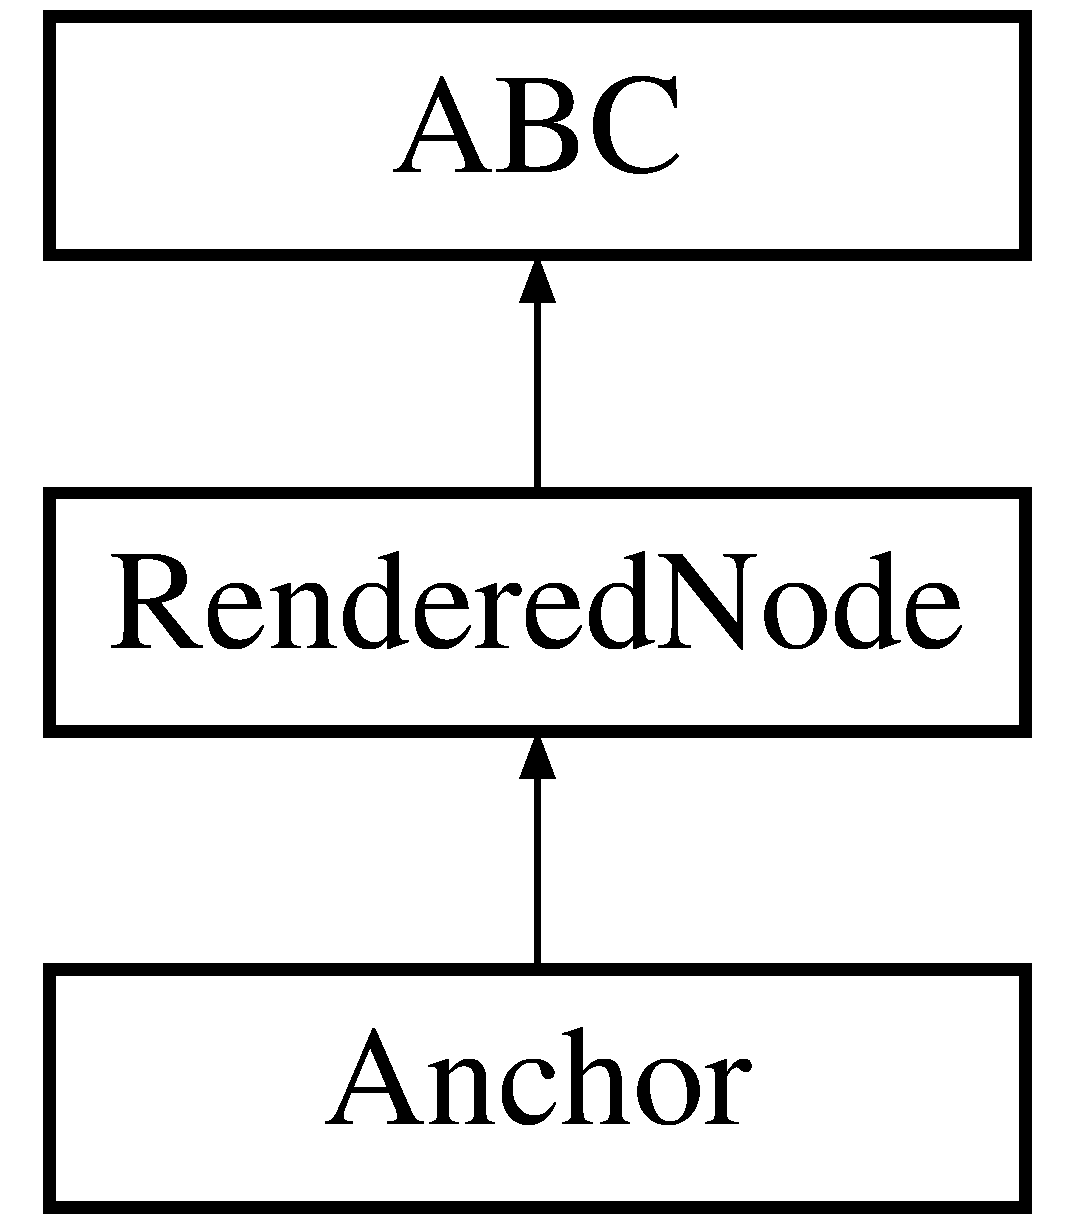
\includegraphics[height=3.000000cm]{classanchor_1_1_anchor}
\end{center}
\end{figure}
\subsection*{Public Member Functions}
\begin{DoxyCompactItemize}
\item 
\mbox{\Hypertarget{classanchor_1_1_anchor_a2cdcced7228de40b037b5e89b94a9873}\label{classanchor_1_1_anchor_a2cdcced7228de40b037b5e89b94a9873}} 
def {\bfseries \+\_\+\+\_\+init\+\_\+\+\_\+} (self, x, y, z, name=\char`\"{}unnamed\char`\"{}, color=\textquotesingle{}red\textquotesingle{})
\item 
\mbox{\Hypertarget{classanchor_1_1_anchor_a89c968c83617e2fca6e64e74c6478b58}\label{classanchor_1_1_anchor_a89c968c83617e2fca6e64e74c6478b58}} 
def {\bfseries get\+\_\+coordinates} (self)
\item 
def \mbox{\hyperlink{classanchor_1_1_anchor_afc59fd77ac0d0375226e77947f7f6624}{set\+\_\+coordinates}} (self, x, y, z)
\item 
def \mbox{\hyperlink{classanchor_1_1_anchor_a09f3f97175c16ea6025da871f653d416}{get\+\_\+\+ID}} (self)
\item 
\mbox{\Hypertarget{classanchor_1_1_anchor_a6f14d5b4ea35ecffbb402607d391ed8f}\label{classanchor_1_1_anchor_a6f14d5b4ea35ecffbb402607d391ed8f}} 
def {\bfseries set\+\_\+color} (self)
\item 
def \mbox{\hyperlink{classanchor_1_1_anchor_a8497086c897585b6ee2234e8728e69e5}{get\+\_\+all\+\_\+distances}} (self)
\item 
def \mbox{\hyperlink{classanchor_1_1_anchor_aa86606ff415bcf3f0e24b2348e925496}{get\+\_\+raw\+\_\+distance}} (self, robotname)
\item 
def \mbox{\hyperlink{classanchor_1_1_anchor_a158cf339169e35c40b2b72862ff5ccf8}{set\+\_\+raw\+\_\+distance}} (self, distance, robotname)
\item 
def \mbox{\hyperlink{classanchor_1_1_anchor_acb50ac316e2abe4093f8e842635467ab}{init\+\_\+rangings}} (self)
\item 
def \mbox{\hyperlink{classanchor_1_1_anchor_a531b5973e62d6cfc80655a893b5155f2}{update\+\_\+rangings}} (self, distance, target)
\item 
def \mbox{\hyperlink{classanchor_1_1_anchor_ad92ac937236e0dcb544cf7913f436ab0}{get\+\_\+distance}} (self, robot\+\_\+id)
\item 
def \mbox{\hyperlink{classanchor_1_1_anchor_a57e1332ae74ab25661204f5fc27c92e7}{set\+\_\+distance}} (self, distance, robot\+\_\+id)
\end{DoxyCompactItemize}
\subsection*{Data Fields}
\begin{DoxyCompactItemize}
\item 
\mbox{\Hypertarget{classanchor_1_1_anchor_a9336ebf25087d91c818ee6e9ec29f8c1}\label{classanchor_1_1_anchor_a9336ebf25087d91c818ee6e9ec29f8c1}} 
{\bfseries x}
\item 
\mbox{\Hypertarget{classanchor_1_1_anchor_a2fb1c5cf58867b5bbc9a1b145a86f3a0}\label{classanchor_1_1_anchor_a2fb1c5cf58867b5bbc9a1b145a86f3a0}} 
{\bfseries y}
\item 
\mbox{\Hypertarget{classanchor_1_1_anchor_a25ed1bcb423b0b7200f485fc5ff71c8e}\label{classanchor_1_1_anchor_a25ed1bcb423b0b7200f485fc5ff71c8e}} 
{\bfseries z}
\item 
\mbox{\Hypertarget{classanchor_1_1_anchor_a37dbdc30935031c05304482e1be89d8f}\label{classanchor_1_1_anchor_a37dbdc30935031c05304482e1be89d8f}} 
{\bfseries color}
\item 
\mbox{\Hypertarget{classanchor_1_1_anchor_ab74e6bf80237ddc4109968cedc58c151}\label{classanchor_1_1_anchor_ab74e6bf80237ddc4109968cedc58c151}} 
{\bfseries name}
\item 
\mbox{\Hypertarget{classanchor_1_1_anchor_ac6c1eeb684483c821de0ec90f6c47cb9}\label{classanchor_1_1_anchor_ac6c1eeb684483c821de0ec90f6c47cb9}} 
{\bfseries shown}
\item 
\mbox{\Hypertarget{classanchor_1_1_anchor_aeda4c5ce97e70fd6df1272e63282fab6}\label{classanchor_1_1_anchor_aeda4c5ce97e70fd6df1272e63282fab6}} 
{\bfseries is\+Active}
\item 
\mbox{\Hypertarget{classanchor_1_1_anchor_a3139244bfb778557108cda2114f91f3f}\label{classanchor_1_1_anchor_a3139244bfb778557108cda2114f91f3f}} 
{\bfseries distance}
\item 
\mbox{\Hypertarget{classanchor_1_1_anchor_a051762e0b74c9578aa0183ebcba61d34}\label{classanchor_1_1_anchor_a051762e0b74c9578aa0183ebcba61d34}} 
{\bfseries raw\+\_\+distance}
\item 
\mbox{\Hypertarget{classanchor_1_1_anchor_a9c7897b1ed7b191c2bb2b3cbcf8c07ff}\label{classanchor_1_1_anchor_a9c7897b1ed7b191c2bb2b3cbcf8c07ff}} 
{\bfseries rangings}
\item 
\mbox{\Hypertarget{classanchor_1_1_anchor_ab22a82fe68a7635a7a7942417682c6f6}\label{classanchor_1_1_anchor_ab22a82fe68a7635a7a7942417682c6f6}} 
{\bfseries correction\+\_\+filter}
\end{DoxyCompactItemize}


\subsection{Detailed Description}
\begin{DoxyVerb}Anchor class - position of the reference station, distances accumalator, distances filtering\end{DoxyVerb}
 

\subsection{Member Function Documentation}
\mbox{\Hypertarget{classanchor_1_1_anchor_a8497086c897585b6ee2234e8728e69e5}\label{classanchor_1_1_anchor_a8497086c897585b6ee2234e8728e69e5}} 
\index{anchor\+::\+Anchor@{anchor\+::\+Anchor}!get\+\_\+all\+\_\+distances@{get\+\_\+all\+\_\+distances}}
\index{get\+\_\+all\+\_\+distances@{get\+\_\+all\+\_\+distances}!anchor\+::\+Anchor@{anchor\+::\+Anchor}}
\subsubsection{\texorpdfstring{get\+\_\+all\+\_\+distances()}{get\_all\_distances()}}
{\footnotesize\ttfamily def get\+\_\+all\+\_\+distances (\begin{DoxyParamCaption}\item[{}]{self }\end{DoxyParamCaption})}

\begin{DoxyVerb}return the distances of the anchor with every robot as a dictionary.\end{DoxyVerb}
 \mbox{\Hypertarget{classanchor_1_1_anchor_ad92ac937236e0dcb544cf7913f436ab0}\label{classanchor_1_1_anchor_ad92ac937236e0dcb544cf7913f436ab0}} 
\index{anchor\+::\+Anchor@{anchor\+::\+Anchor}!get\+\_\+distance@{get\+\_\+distance}}
\index{get\+\_\+distance@{get\+\_\+distance}!anchor\+::\+Anchor@{anchor\+::\+Anchor}}
\subsubsection{\texorpdfstring{get\+\_\+distance()}{get\_distance()}}
{\footnotesize\ttfamily def get\+\_\+distance (\begin{DoxyParamCaption}\item[{}]{self,  }\item[{}]{robot\+\_\+id }\end{DoxyParamCaption})}

\begin{DoxyVerb}gets the filtered distance between the anchor and the given robot\end{DoxyVerb}
 \mbox{\Hypertarget{classanchor_1_1_anchor_a09f3f97175c16ea6025da871f653d416}\label{classanchor_1_1_anchor_a09f3f97175c16ea6025da871f653d416}} 
\index{anchor\+::\+Anchor@{anchor\+::\+Anchor}!get\+\_\+\+ID@{get\+\_\+\+ID}}
\index{get\+\_\+\+ID@{get\+\_\+\+ID}!anchor\+::\+Anchor@{anchor\+::\+Anchor}}
\subsubsection{\texorpdfstring{get\+\_\+\+I\+D()}{get\_ID()}}
{\footnotesize\ttfamily def get\+\_\+\+ID (\begin{DoxyParamCaption}\item[{}]{self }\end{DoxyParamCaption})}

\begin{DoxyVerb}returns anchor ID\end{DoxyVerb}
 \mbox{\Hypertarget{classanchor_1_1_anchor_aa86606ff415bcf3f0e24b2348e925496}\label{classanchor_1_1_anchor_aa86606ff415bcf3f0e24b2348e925496}} 
\index{anchor\+::\+Anchor@{anchor\+::\+Anchor}!get\+\_\+raw\+\_\+distance@{get\+\_\+raw\+\_\+distance}}
\index{get\+\_\+raw\+\_\+distance@{get\+\_\+raw\+\_\+distance}!anchor\+::\+Anchor@{anchor\+::\+Anchor}}
\subsubsection{\texorpdfstring{get\+\_\+raw\+\_\+distance()}{get\_raw\_distance()}}
{\footnotesize\ttfamily def get\+\_\+raw\+\_\+distance (\begin{DoxyParamCaption}\item[{}]{self,  }\item[{}]{robotname }\end{DoxyParamCaption})}

\begin{DoxyVerb}gets the unfiltered distance between the anchor and the given robot\end{DoxyVerb}
 \mbox{\Hypertarget{classanchor_1_1_anchor_acb50ac316e2abe4093f8e842635467ab}\label{classanchor_1_1_anchor_acb50ac316e2abe4093f8e842635467ab}} 
\index{anchor\+::\+Anchor@{anchor\+::\+Anchor}!init\+\_\+rangings@{init\+\_\+rangings}}
\index{init\+\_\+rangings@{init\+\_\+rangings}!anchor\+::\+Anchor@{anchor\+::\+Anchor}}
\subsubsection{\texorpdfstring{init\+\_\+rangings()}{init\_rangings()}}
{\footnotesize\ttfamily def init\+\_\+rangings (\begin{DoxyParamCaption}\item[{}]{self }\end{DoxyParamCaption})}

\begin{DoxyVerb}generates an entry for each robot id in the rangings dictionary\end{DoxyVerb}
 \mbox{\Hypertarget{classanchor_1_1_anchor_afc59fd77ac0d0375226e77947f7f6624}\label{classanchor_1_1_anchor_afc59fd77ac0d0375226e77947f7f6624}} 
\index{anchor\+::\+Anchor@{anchor\+::\+Anchor}!set\+\_\+coordinates@{set\+\_\+coordinates}}
\index{set\+\_\+coordinates@{set\+\_\+coordinates}!anchor\+::\+Anchor@{anchor\+::\+Anchor}}
\subsubsection{\texorpdfstring{set\+\_\+coordinates()}{set\_coordinates()}}
{\footnotesize\ttfamily def set\+\_\+coordinates (\begin{DoxyParamCaption}\item[{}]{self,  }\item[{}]{x,  }\item[{}]{y,  }\item[{}]{z }\end{DoxyParamCaption})}

\begin{DoxyVerb}Sets the anchor coordinates. Should be used carefully; this will lead to errors in the localization algorithm.
Use move_node instead if you wish to move only the node representation in the 3D engine\end{DoxyVerb}
 \mbox{\Hypertarget{classanchor_1_1_anchor_a57e1332ae74ab25661204f5fc27c92e7}\label{classanchor_1_1_anchor_a57e1332ae74ab25661204f5fc27c92e7}} 
\index{anchor\+::\+Anchor@{anchor\+::\+Anchor}!set\+\_\+distance@{set\+\_\+distance}}
\index{set\+\_\+distance@{set\+\_\+distance}!anchor\+::\+Anchor@{anchor\+::\+Anchor}}
\subsubsection{\texorpdfstring{set\+\_\+distance()}{set\_distance()}}
{\footnotesize\ttfamily def set\+\_\+distance (\begin{DoxyParamCaption}\item[{}]{self,  }\item[{}]{distance,  }\item[{}]{robot\+\_\+id }\end{DoxyParamCaption})}

\begin{DoxyVerb}sets the filtered distance between the anchor and the given robot\end{DoxyVerb}
 \mbox{\Hypertarget{classanchor_1_1_anchor_a158cf339169e35c40b2b72862ff5ccf8}\label{classanchor_1_1_anchor_a158cf339169e35c40b2b72862ff5ccf8}} 
\index{anchor\+::\+Anchor@{anchor\+::\+Anchor}!set\+\_\+raw\+\_\+distance@{set\+\_\+raw\+\_\+distance}}
\index{set\+\_\+raw\+\_\+distance@{set\+\_\+raw\+\_\+distance}!anchor\+::\+Anchor@{anchor\+::\+Anchor}}
\subsubsection{\texorpdfstring{set\+\_\+raw\+\_\+distance()}{set\_raw\_distance()}}
{\footnotesize\ttfamily def set\+\_\+raw\+\_\+distance (\begin{DoxyParamCaption}\item[{}]{self,  }\item[{}]{distance,  }\item[{}]{robotname }\end{DoxyParamCaption})}

\begin{DoxyVerb}sets the unfiltered distance between the anchor and the given robot\end{DoxyVerb}
 \mbox{\Hypertarget{classanchor_1_1_anchor_a531b5973e62d6cfc80655a893b5155f2}\label{classanchor_1_1_anchor_a531b5973e62d6cfc80655a893b5155f2}} 
\index{anchor\+::\+Anchor@{anchor\+::\+Anchor}!update\+\_\+rangings@{update\+\_\+rangings}}
\index{update\+\_\+rangings@{update\+\_\+rangings}!anchor\+::\+Anchor@{anchor\+::\+Anchor}}
\subsubsection{\texorpdfstring{update\+\_\+rangings()}{update\_rangings()}}
{\footnotesize\ttfamily def update\+\_\+rangings (\begin{DoxyParamCaption}\item[{}]{self,  }\item[{}]{distance,  }\item[{}]{target }\end{DoxyParamCaption})}

\begin{DoxyVerb}updates the list of the last NB_RANGINGS rangings\end{DoxyVerb}
 

The documentation for this class was generated from the following file\+:\begin{DoxyCompactItemize}
\item 
C\+:/\+Users/pestourb/\+Documents/\+Git\+Hub/\+Secure\+Loc/anchor.\+py\end{DoxyCompactItemize}

\hypertarget{classapplication_1_1_application}{}\section{Application Class Reference}
\label{classapplication_1_1_application}\index{Application@{Application}}
Inheritance diagram for Application\+:\begin{figure}[H]
\begin{center}
\leavevmode
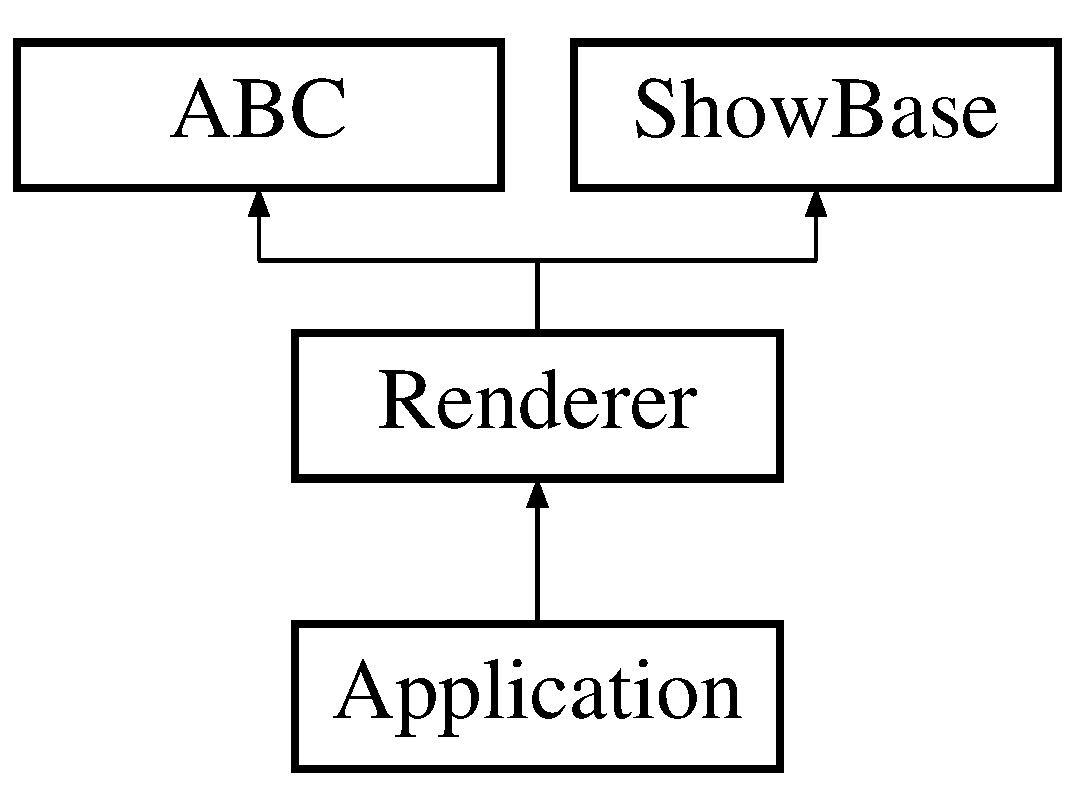
\includegraphics[height=3.000000cm]{classapplication_1_1_application}
\end{center}
\end{figure}
\subsection*{Public Member Functions}
\begin{DoxyCompactItemize}
\item 
\mbox{\Hypertarget{classapplication_1_1_application_ae64f0875afe3067b97ba370b354b9213}\label{classapplication_1_1_application_ae64f0875afe3067b97ba370b354b9213}} 
def {\bfseries \+\_\+\+\_\+init\+\_\+\+\_\+} (self)
\item 
def \mbox{\hyperlink{classapplication_1_1_application_a723c0a1022badcd24965be09a1ccad83}{U\+I\+\_\+management\+\_\+task}} (self, task)
\item 
def \mbox{\hyperlink{classapplication_1_1_application_a919e7c637c4e2c70b80ea71ff708e0c5}{add\+\_\+anchor}} (self, anchor\+\_\+pos)
\item 
def \mbox{\hyperlink{classapplication_1_1_application_afb149cfcea0378638df7b16662fb4516}{add\+\_\+tag}} (self, tag\+\_\+pos)
\item 
def \mbox{\hyperlink{classapplication_1_1_application_a44b040db1450b3e52875b18bf3c397ab}{create\+\_\+world}} (self)
\item 
def \mbox{\hyperlink{classapplication_1_1_application_abd46271df4663c0a6eafd65cc0225619}{create\+\_\+moving\+\_\+entities}} (self)
\item 
def \mbox{\hyperlink{classapplication_1_1_application_a5d5f203a22d435fe3ba8f20a98912951}{init\+\_\+mqtt}} (self)
\item 
def \mbox{\hyperlink{classapplication_1_1_application_ac8badcf7fda4f70c2c93bfe0e55edcb3}{on\+\_\+message}} (self, mqttc, obj, msg)
\item 
def \mbox{\hyperlink{classapplication_1_1_application_a875504ef90230b137861e39cc7ba6c7f}{init\+\_\+logs}} (self)
\item 
def \mbox{\hyperlink{classapplication_1_1_application_a9748ebedda92b7e9328841d6633080b6}{log\+\_\+dataset}} (self, \mbox{\hyperlink{classjson_structures_1_1dataset}{dataset}})
\item 
def \mbox{\hyperlink{classapplication_1_1_application_a976549ccc76753bc31f99185a789a595}{log\+\_\+pos}} (self, pos)
\item 
def \mbox{\hyperlink{classapplication_1_1_application_a5532bf93412434e87215e5dba8f0c366}{check\+Inputs}} (self)
\item 
def \mbox{\hyperlink{classapplication_1_1_application_a87078a437ca2d9fb5c7c7e3f3f964d7b}{update\+\_\+positions\+\_\+task}} (self, task)
\item 
def \mbox{\hyperlink{classapplication_1_1_application_a3b37792e871ae0aff20a7fc504b29458}{simulation\+\_\+layer}} (self, tag)
\item 
def \mbox{\hyperlink{classapplication_1_1_application_afded811885b0390450238ee8487d992a}{get\+\_\+rp}} (self, tabfile=\char`\"{}rp.\+tab\char`\"{})
\item 
def \mbox{\hyperlink{classapplication_1_1_application_aabeebafd4c55db0de5b62920f912b428}{update\+\_\+sock\+\_\+task}} (self, task)
\item 
def \mbox{\hyperlink{classapplication_1_1_application_aadd900346b1bd5c962657a1566f9fbb7}{manage\+\_\+measurements}} (self)
\end{DoxyCompactItemize}
\subsection*{Data Fields}
\begin{DoxyCompactItemize}
\item 
\mbox{\Hypertarget{classapplication_1_1_application_a4ccc9b09cd5009aceaa248cf636be51d}\label{classapplication_1_1_application_a4ccc9b09cd5009aceaa248cf636be51d}} 
{\bfseries tags}
\item 
\mbox{\Hypertarget{classapplication_1_1_application_aa6981c1c0f4722a428c855b7ff4603d4}\label{classapplication_1_1_application_aa6981c1c0f4722a428c855b7ff4603d4}} 
{\bfseries logs\+\_\+pipe}
\item 
\mbox{\Hypertarget{classapplication_1_1_application_aba54450ad49ad1b46e29721241611d50}\label{classapplication_1_1_application_aba54450ad49ad1b46e29721241611d50}} 
{\bfseries anchors}
\item 
\mbox{\Hypertarget{classapplication_1_1_application_a5122b177c209e63e9c26f64b84f44a68}\label{classapplication_1_1_application_a5122b177c209e63e9c26f64b84f44a68}} 
{\bfseries pos\+\_\+array}
\item 
\mbox{\Hypertarget{classapplication_1_1_application_a9c7897b1ed7b191c2bb2b3cbcf8c07ff}\label{classapplication_1_1_application_a9c7897b1ed7b191c2bb2b3cbcf8c07ff}} 
{\bfseries rangings}
\item 
\mbox{\Hypertarget{classapplication_1_1_application_a6f9bc23a0e2554f19b4036e10d681977}\label{classapplication_1_1_application_a6f9bc23a0e2554f19b4036e10d681977}} 
{\bfseries ranging\+\_\+counter}
\item 
\mbox{\Hypertarget{classapplication_1_1_application_a63baf4774f1048f9dbfd5760bde1a3ad}\label{classapplication_1_1_application_a63baf4774f1048f9dbfd5760bde1a3ad}} 
{\bfseries mes\+\_\+counter}
\item 
\mbox{\Hypertarget{classapplication_1_1_application_ae55e74a083b645560070a790ecfaf83d}\label{classapplication_1_1_application_ae55e74a083b645560070a790ecfaf83d}} 
{\bfseries ref\+\_\+points}
\item 
\mbox{\Hypertarget{classapplication_1_1_application_a3eca7195563a4c365bb41c312d8f7d3c}\label{classapplication_1_1_application_a3eca7195563a4c365bb41c312d8f7d3c}} 
{\bfseries rp}
\item 
\mbox{\Hypertarget{classapplication_1_1_application_a68f4061e1fd07ed7c7042d2afa9b8286}\label{classapplication_1_1_application_a68f4061e1fd07ed7c7042d2afa9b8286}} 
{\bfseries threads\+\_\+pipe}
\item 
\mbox{\Hypertarget{classapplication_1_1_application_ad268f8672c706f6492e684c02b6e3d6e}\label{classapplication_1_1_application_ad268f8672c706f6492e684c02b6e3d6e}} 
{\bfseries filters}
\item 
\mbox{\Hypertarget{classapplication_1_1_application_aaa50d80c7b704568ea8315d5160a39d4}\label{classapplication_1_1_application_aaa50d80c7b704568ea8315d5160a39d4}} 
\mbox{\hyperlink{classapplication_1_1_application_aaa50d80c7b704568ea8315d5160a39d4}{simulator}}
\begin{DoxyCompactList}\small\item\em \mbox{\hyperlink{namespace_simulation}{Simulation}} layer config. \end{DoxyCompactList}\item 
\mbox{\Hypertarget{classapplication_1_1_application_aa98e4feadd3ff49c54b9494418d0c1b9}\label{classapplication_1_1_application_aa98e4feadd3ff49c54b9494418d0c1b9}} 
{\bfseries keep\+\_\+dataset}
\item 
\mbox{\Hypertarget{classapplication_1_1_application_a905479d79c2aa8410d2fc374bc75cc5b}\label{classapplication_1_1_application_a905479d79c2aa8410d2fc374bc75cc5b}} 
\mbox{\hyperlink{classapplication_1_1_application_a905479d79c2aa8410d2fc374bc75cc5b}{menu}}
\begin{DoxyCompactList}\small\item\em menu configuration \end{DoxyCompactList}\item 
\mbox{\Hypertarget{classapplication_1_1_application_a0cce6087c1ee78f78ebb7e4b338dd790}\label{classapplication_1_1_application_a0cce6087c1ee78f78ebb7e4b338dd790}} 
{\bfseries menu\+\_\+pipe}
\item 
\mbox{\Hypertarget{classapplication_1_1_application_a17a813ff016f566e53dfb54c93ba2913}\label{classapplication_1_1_application_a17a813ff016f566e53dfb54c93ba2913}} 
\mbox{\hyperlink{classapplication_1_1_application_a17a813ff016f566e53dfb54c93ba2913}{dataset}}
\begin{DoxyCompactList}\small\item\em logs config \end{DoxyCompactList}\item 
\mbox{\Hypertarget{classapplication_1_1_application_a1455b045e2343939799f2ff658d8e39c}\label{classapplication_1_1_application_a1455b045e2343939799f2ff658d8e39c}} 
{\bfseries log\+\_\+flag}
\item 
\mbox{\Hypertarget{classapplication_1_1_application_a7a1f94eb5d0fcb264b366614d7525f87}\label{classapplication_1_1_application_a7a1f94eb5d0fcb264b366614d7525f87}} 
{\bfseries exit\+\_\+flag}
\item 
\mbox{\Hypertarget{classapplication_1_1_application_ad604cff3eb5d475cdc9f8eb5ab570fee}\label{classapplication_1_1_application_ad604cff3eb5d475cdc9f8eb5ab570fee}} 
{\bfseries done}
\item 
\mbox{\Hypertarget{classapplication_1_1_application_aa42a09469de866c0b3eecb8e90dc344f}\label{classapplication_1_1_application_aa42a09469de866c0b3eecb8e90dc344f}} 
{\bfseries log2play}
\item 
\mbox{\Hypertarget{classapplication_1_1_application_a98121304a3885b9699b36513af09106b}\label{classapplication_1_1_application_a98121304a3885b9699b36513af09106b}} 
{\bfseries playback\+\_\+path}
\item 
\mbox{\Hypertarget{classapplication_1_1_application_a41f34ddde8a8c59af60372d9f5e72d33}\label{classapplication_1_1_application_a41f34ddde8a8c59af60372d9f5e72d33}} 
{\bfseries playback\+\_\+rangings}
\item 
\mbox{\Hypertarget{classapplication_1_1_application_a5fa42e2715ac629edc61832574f0c399}\label{classapplication_1_1_application_a5fa42e2715ac629edc61832574f0c399}} 
{\bfseries playback\+\_\+counter}
\item 
\mbox{\Hypertarget{classapplication_1_1_application_ab1c5110ce9bc51d1e16d285ab470a89a}\label{classapplication_1_1_application_ab1c5110ce9bc51d1e16d285ab470a89a}} 
{\bfseries mqttc}
\item 
\mbox{\Hypertarget{classapplication_1_1_application_ad5377048bcfeeababab31687e9bbda03}\label{classapplication_1_1_application_ad5377048bcfeeababab31687e9bbda03}} 
{\bfseries logs\+\_\+mqtt}
\item 
\mbox{\Hypertarget{classapplication_1_1_application_a4f5f05e7cf862586d58b123ebeac3e62}\label{classapplication_1_1_application_a4f5f05e7cf862586d58b123ebeac3e62}} 
{\bfseries logs\+\_\+pos}
\item 
\mbox{\Hypertarget{classapplication_1_1_application_ad5d8bd2f2c7ba06f51a39486c579491f}\label{classapplication_1_1_application_ad5d8bd2f2c7ba06f51a39486c579491f}} 
{\bfseries logs\+\_\+rangings}
\item 
\mbox{\Hypertarget{classapplication_1_1_application_a95d27c454bae5de9e80962221646154e}\label{classapplication_1_1_application_a95d27c454bae5de9e80962221646154e}} 
\mbox{\hyperlink{classapplication_1_1_application_a95d27c454bae5de9e80962221646154e}{world}}
\begin{DoxyCompactList}\small\item\em anchor creation \end{DoxyCompactList}\item 
\mbox{\Hypertarget{classapplication_1_1_application_aca5bd7c00943f5ff8a4cf50e52782628}\label{classapplication_1_1_application_aca5bd7c00943f5ff8a4cf50e52782628}} 
{\bfseries processed\+\_\+robot}
\end{DoxyCompactItemize}


\subsection{Detailed Description}
\begin{DoxyVerb}Main application class\end{DoxyVerb}
 

\subsection{Member Function Documentation}
\mbox{\Hypertarget{classapplication_1_1_application_a919e7c637c4e2c70b80ea71ff708e0c5}\label{classapplication_1_1_application_a919e7c637c4e2c70b80ea71ff708e0c5}} 
\index{application\+::\+Application@{application\+::\+Application}!add\+\_\+anchor@{add\+\_\+anchor}}
\index{add\+\_\+anchor@{add\+\_\+anchor}!application\+::\+Application@{application\+::\+Application}}
\subsubsection{\texorpdfstring{add\+\_\+anchor()}{add\_anchor()}}
{\footnotesize\ttfamily def add\+\_\+anchor (\begin{DoxyParamCaption}\item[{}]{self,  }\item[{}]{anchor\+\_\+pos }\end{DoxyParamCaption})}

\begin{DoxyVerb}adds an anchor to the current world. Should be used to create a fictive anchor\end{DoxyVerb}
 \mbox{\Hypertarget{classapplication_1_1_application_afb149cfcea0378638df7b16662fb4516}\label{classapplication_1_1_application_afb149cfcea0378638df7b16662fb4516}} 
\index{application\+::\+Application@{application\+::\+Application}!add\+\_\+tag@{add\+\_\+tag}}
\index{add\+\_\+tag@{add\+\_\+tag}!application\+::\+Application@{application\+::\+Application}}
\subsubsection{\texorpdfstring{add\+\_\+tag()}{add\_tag()}}
{\footnotesize\ttfamily def add\+\_\+tag (\begin{DoxyParamCaption}\item[{}]{self,  }\item[{}]{tag\+\_\+pos }\end{DoxyParamCaption})}

\begin{DoxyVerb}adds an tag to the current world. Should be used to create a fictive tag\end{DoxyVerb}
 \mbox{\Hypertarget{classapplication_1_1_application_a5532bf93412434e87215e5dba8f0c366}\label{classapplication_1_1_application_a5532bf93412434e87215e5dba8f0c366}} 
\index{application\+::\+Application@{application\+::\+Application}!check\+Inputs@{check\+Inputs}}
\index{check\+Inputs@{check\+Inputs}!application\+::\+Application@{application\+::\+Application}}
\subsubsection{\texorpdfstring{check\+Inputs()}{checkInputs()}}
{\footnotesize\ttfamily def check\+Inputs (\begin{DoxyParamCaption}\item[{}]{self }\end{DoxyParamCaption})}

\begin{DoxyVerb}manages user keyboard interaction \end{DoxyVerb}
 \mbox{\Hypertarget{classapplication_1_1_application_abd46271df4663c0a6eafd65cc0225619}\label{classapplication_1_1_application_abd46271df4663c0a6eafd65cc0225619}} 
\index{application\+::\+Application@{application\+::\+Application}!create\+\_\+moving\+\_\+entities@{create\+\_\+moving\+\_\+entities}}
\index{create\+\_\+moving\+\_\+entities@{create\+\_\+moving\+\_\+entities}!application\+::\+Application@{application\+::\+Application}}
\subsubsection{\texorpdfstring{create\+\_\+moving\+\_\+entities()}{create\_moving\_entities()}}
{\footnotesize\ttfamily def create\+\_\+moving\+\_\+entities (\begin{DoxyParamCaption}\item[{}]{self }\end{DoxyParamCaption})}

\begin{DoxyVerb}Create moving entities\end{DoxyVerb}
 \mbox{\Hypertarget{classapplication_1_1_application_a44b040db1450b3e52875b18bf3c397ab}\label{classapplication_1_1_application_a44b040db1450b3e52875b18bf3c397ab}} 
\index{application\+::\+Application@{application\+::\+Application}!create\+\_\+world@{create\+\_\+world}}
\index{create\+\_\+world@{create\+\_\+world}!application\+::\+Application@{application\+::\+Application}}
\subsubsection{\texorpdfstring{create\+\_\+world()}{create\_world()}}
{\footnotesize\ttfamily def create\+\_\+world (\begin{DoxyParamCaption}\item[{}]{self }\end{DoxyParamCaption})}

\begin{DoxyVerb}Creates the 3D world in which entities will evolve\end{DoxyVerb}
 \mbox{\Hypertarget{classapplication_1_1_application_afded811885b0390450238ee8487d992a}\label{classapplication_1_1_application_afded811885b0390450238ee8487d992a}} 
\index{application\+::\+Application@{application\+::\+Application}!get\+\_\+rp@{get\+\_\+rp}}
\index{get\+\_\+rp@{get\+\_\+rp}!application\+::\+Application@{application\+::\+Application}}
\subsubsection{\texorpdfstring{get\+\_\+rp()}{get\_rp()}}
{\footnotesize\ttfamily def get\+\_\+rp (\begin{DoxyParamCaption}\item[{}]{self,  }\item[{}]{tabfile = {\ttfamily \char`\"{}rp.tab\char`\"{}} }\end{DoxyParamCaption})}

\begin{DoxyVerb}For measurements mode only. Gets the reference points in the configuration file\end{DoxyVerb}
 \mbox{\Hypertarget{classapplication_1_1_application_a875504ef90230b137861e39cc7ba6c7f}\label{classapplication_1_1_application_a875504ef90230b137861e39cc7ba6c7f}} 
\index{application\+::\+Application@{application\+::\+Application}!init\+\_\+logs@{init\+\_\+logs}}
\index{init\+\_\+logs@{init\+\_\+logs}!application\+::\+Application@{application\+::\+Application}}
\subsubsection{\texorpdfstring{init\+\_\+logs()}{init\_logs()}}
{\footnotesize\ttfamily def init\+\_\+logs (\begin{DoxyParamCaption}\item[{}]{self }\end{DoxyParamCaption})}

\begin{DoxyVerb}initializes json logs with current date & time, and creates the
pipe for loggin thread communication\end{DoxyVerb}
 \mbox{\Hypertarget{classapplication_1_1_application_a5d5f203a22d435fe3ba8f20a98912951}\label{classapplication_1_1_application_a5d5f203a22d435fe3ba8f20a98912951}} 
\index{application\+::\+Application@{application\+::\+Application}!init\+\_\+mqtt@{init\+\_\+mqtt}}
\index{init\+\_\+mqtt@{init\+\_\+mqtt}!application\+::\+Application@{application\+::\+Application}}
\subsubsection{\texorpdfstring{init\+\_\+mqtt()}{init\_mqtt()}}
{\footnotesize\ttfamily def init\+\_\+mqtt (\begin{DoxyParamCaption}\item[{}]{self }\end{DoxyParamCaption})}

\begin{DoxyVerb}creates the mqtt client and handles the subscriptions\end{DoxyVerb}
 \mbox{\Hypertarget{classapplication_1_1_application_a9748ebedda92b7e9328841d6633080b6}\label{classapplication_1_1_application_a9748ebedda92b7e9328841d6633080b6}} 
\index{application\+::\+Application@{application\+::\+Application}!log\+\_\+dataset@{log\+\_\+dataset}}
\index{log\+\_\+dataset@{log\+\_\+dataset}!application\+::\+Application@{application\+::\+Application}}
\subsubsection{\texorpdfstring{log\+\_\+dataset()}{log\_dataset()}}
{\footnotesize\ttfamily def log\+\_\+dataset (\begin{DoxyParamCaption}\item[{}]{self,  }\item[{}]{dataset }\end{DoxyParamCaption})}

\begin{DoxyVerb}writes the last dataset received in logs file\end{DoxyVerb}
 \mbox{\Hypertarget{classapplication_1_1_application_a976549ccc76753bc31f99185a789a595}\label{classapplication_1_1_application_a976549ccc76753bc31f99185a789a595}} 
\index{application\+::\+Application@{application\+::\+Application}!log\+\_\+pos@{log\+\_\+pos}}
\index{log\+\_\+pos@{log\+\_\+pos}!application\+::\+Application@{application\+::\+Application}}
\subsubsection{\texorpdfstring{log\+\_\+pos()}{log\_pos()}}
{\footnotesize\ttfamily def log\+\_\+pos (\begin{DoxyParamCaption}\item[{}]{self,  }\item[{}]{pos }\end{DoxyParamCaption})}

\begin{DoxyVerb}writes the id of the robot and its last pos recorded in logs file\end{DoxyVerb}
 \mbox{\Hypertarget{classapplication_1_1_application_aadd900346b1bd5c962657a1566f9fbb7}\label{classapplication_1_1_application_aadd900346b1bd5c962657a1566f9fbb7}} 
\index{application\+::\+Application@{application\+::\+Application}!manage\+\_\+measurements@{manage\+\_\+measurements}}
\index{manage\+\_\+measurements@{manage\+\_\+measurements}!application\+::\+Application@{application\+::\+Application}}
\subsubsection{\texorpdfstring{manage\+\_\+measurements()}{manage\_measurements()}}
{\footnotesize\ttfamily def manage\+\_\+measurements (\begin{DoxyParamCaption}\item[{}]{self }\end{DoxyParamCaption})}

\begin{DoxyVerb}handles the pace of measurements. Measurements modes consist of series of measures separated by short rests.
The duration can be set by the user\end{DoxyVerb}
 \mbox{\Hypertarget{classapplication_1_1_application_ac8badcf7fda4f70c2c93bfe0e55edcb3}\label{classapplication_1_1_application_ac8badcf7fda4f70c2c93bfe0e55edcb3}} 
\index{application\+::\+Application@{application\+::\+Application}!on\+\_\+message@{on\+\_\+message}}
\index{on\+\_\+message@{on\+\_\+message}!application\+::\+Application@{application\+::\+Application}}
\subsubsection{\texorpdfstring{on\+\_\+message()}{on\_message()}}
{\footnotesize\ttfamily def on\+\_\+message (\begin{DoxyParamCaption}\item[{}]{self,  }\item[{}]{mqttc,  }\item[{}]{obj,  }\item[{}]{msg }\end{DoxyParamCaption})}

\begin{DoxyVerb}handles data resfreshing when a mqtt message is received\end{DoxyVerb}
 \mbox{\Hypertarget{classapplication_1_1_application_a3b37792e871ae0aff20a7fc504b29458}\label{classapplication_1_1_application_a3b37792e871ae0aff20a7fc504b29458}} 
\index{application\+::\+Application@{application\+::\+Application}!simulation\+\_\+layer@{simulation\+\_\+layer}}
\index{simulation\+\_\+layer@{simulation\+\_\+layer}!application\+::\+Application@{application\+::\+Application}}
\subsubsection{\texorpdfstring{simulation\+\_\+layer()}{simulation\_layer()}}
{\footnotesize\ttfamily def simulation\+\_\+layer (\begin{DoxyParamCaption}\item[{}]{self,  }\item[{}]{tag }\end{DoxyParamCaption})}

\begin{DoxyVerb}handles all the tasks related to the simulator\end{DoxyVerb}
 \mbox{\Hypertarget{classapplication_1_1_application_a723c0a1022badcd24965be09a1ccad83}\label{classapplication_1_1_application_a723c0a1022badcd24965be09a1ccad83}} 
\index{application\+::\+Application@{application\+::\+Application}!U\+I\+\_\+management\+\_\+task@{U\+I\+\_\+management\+\_\+task}}
\index{U\+I\+\_\+management\+\_\+task@{U\+I\+\_\+management\+\_\+task}!application\+::\+Application@{application\+::\+Application}}
\subsubsection{\texorpdfstring{U\+I\+\_\+management\+\_\+task()}{UI\_management\_task()}}
{\footnotesize\ttfamily def U\+I\+\_\+management\+\_\+task (\begin{DoxyParamCaption}\item[{}]{self,  }\item[{}]{task }\end{DoxyParamCaption})}

\begin{DoxyVerb}Handles user inputs; refresh rate can be set in parameters\end{DoxyVerb}
 \mbox{\Hypertarget{classapplication_1_1_application_a87078a437ca2d9fb5c7c7e3f3f964d7b}\label{classapplication_1_1_application_a87078a437ca2d9fb5c7c7e3f3f964d7b}} 
\index{application\+::\+Application@{application\+::\+Application}!update\+\_\+positions\+\_\+task@{update\+\_\+positions\+\_\+task}}
\index{update\+\_\+positions\+\_\+task@{update\+\_\+positions\+\_\+task}!application\+::\+Application@{application\+::\+Application}}
\subsubsection{\texorpdfstring{update\+\_\+positions\+\_\+task()}{update\_positions\_task()}}
{\footnotesize\ttfamily def update\+\_\+positions\+\_\+task (\begin{DoxyParamCaption}\item[{}]{self,  }\item[{}]{task }\end{DoxyParamCaption})}

\begin{DoxyVerb}Updates moving entities positions\end{DoxyVerb}
 \mbox{\Hypertarget{classapplication_1_1_application_aabeebafd4c55db0de5b62920f912b428}\label{classapplication_1_1_application_aabeebafd4c55db0de5b62920f912b428}} 
\index{application\+::\+Application@{application\+::\+Application}!update\+\_\+sock\+\_\+task@{update\+\_\+sock\+\_\+task}}
\index{update\+\_\+sock\+\_\+task@{update\+\_\+sock\+\_\+task}!application\+::\+Application@{application\+::\+Application}}
\subsubsection{\texorpdfstring{update\+\_\+sock\+\_\+task()}{update\_sock\_task()}}
{\footnotesize\ttfamily def update\+\_\+sock\+\_\+task (\begin{DoxyParamCaption}\item[{}]{self,  }\item[{}]{task }\end{DoxyParamCaption})}

\begin{DoxyVerb}Asks server newest positions of entities\end{DoxyVerb}
\begin{DoxyVerb}In playback mode the socket is bypassed and ranging resultd are obtained directly from the log file\end{DoxyVerb}
 

The documentation for this class was generated from the following file\+:\begin{DoxyCompactItemize}
\item 
C\+:/\+Users/pestourb/\+Documents/\+Git\+Hub/\+Secure\+Loc/application.\+py\end{DoxyCompactItemize}

\hypertarget{class_attacks_1_1_attack}{}\section{Attack Class Reference}
\label{class_attacks_1_1_attack}\index{Attack@{Attack}}
\subsection*{Public Member Functions}
\begin{DoxyCompactItemize}
\item 
\mbox{\Hypertarget{class_attacks_1_1_attack_ac7e11b0c699f3512b8b1ae903ba3944c}\label{class_attacks_1_1_attack_ac7e11b0c699f3512b8b1ae903ba3944c}} 
def {\bfseries \+\_\+\+\_\+init\+\_\+\+\_\+} (self, success\+\_\+rate, dos\+\_\+rate, distance\+\_\+distribution)
\item 
def \mbox{\hyperlink{class_attacks_1_1_attack_ab16da2c66772b1363a9db1e338f1e445}{apply}} (self, data)
\item 
def \mbox{\hyperlink{class_attacks_1_1_attack_a648687d12cef0a0d27e179d15311187d}{distance\+\_\+distribution\+\_\+apply}} (self, distance)
\end{DoxyCompactItemize}
\subsection*{Data Fields}
\begin{DoxyCompactItemize}
\item 
\mbox{\Hypertarget{class_attacks_1_1_attack_a7c855ec6d163e10846e723e0d5d96fce}\label{class_attacks_1_1_attack_a7c855ec6d163e10846e723e0d5d96fce}} 
{\bfseries success\+\_\+rate}
\item 
\mbox{\Hypertarget{class_attacks_1_1_attack_a2ab94bd38ebfc77d36946b4e6007ecfa}\label{class_attacks_1_1_attack_a2ab94bd38ebfc77d36946b4e6007ecfa}} 
{\bfseries dos\+\_\+rate}
\item 
\mbox{\Hypertarget{class_attacks_1_1_attack_a590a35947be7c58e794475226eba6178}\label{class_attacks_1_1_attack_a590a35947be7c58e794475226eba6178}} 
{\bfseries distance\+\_\+distribution}
\item 
\mbox{\Hypertarget{class_attacks_1_1_attack_a7a229a4786deeddd59c6091247a8c8a6}\label{class_attacks_1_1_attack_a7a229a4786deeddd59c6091247a8c8a6}} 
{\bfseries offset}
\item 
\mbox{\Hypertarget{class_attacks_1_1_attack_aca9a7ee02fb8663e9e2971ca4052b0c6}\label{class_attacks_1_1_attack_aca9a7ee02fb8663e9e2971ca4052b0c6}} 
{\bfseries targets}
\end{DoxyCompactItemize}


\subsection{Detailed Description}
\begin{DoxyVerb}An attack is represented by three parameters:
    - Success rate, i.e., probability that the attack generates modifies the distance output
    - DoS rate, i.e., probability that the attack denies a given sample
    - Distance distribution, i.e., in case of distance how the distance will be modified. This is given as a probabilistic distribution\end{DoxyVerb}
 

\subsection{Member Function Documentation}
\mbox{\Hypertarget{class_attacks_1_1_attack_ab16da2c66772b1363a9db1e338f1e445}\label{class_attacks_1_1_attack_ab16da2c66772b1363a9db1e338f1e445}} 
\index{Attacks\+::\+Attack@{Attacks\+::\+Attack}!apply@{apply}}
\index{apply@{apply}!Attacks\+::\+Attack@{Attacks\+::\+Attack}}
\subsubsection{\texorpdfstring{apply()}{apply()}}
{\footnotesize\ttfamily def apply (\begin{DoxyParamCaption}\item[{}]{self,  }\item[{}]{data }\end{DoxyParamCaption})}

\begin{DoxyVerb}Simulates the effect of an attack on a dataset. True if dataset if kept, false otherwise\end{DoxyVerb}
 \mbox{\Hypertarget{class_attacks_1_1_attack_a648687d12cef0a0d27e179d15311187d}\label{class_attacks_1_1_attack_a648687d12cef0a0d27e179d15311187d}} 
\index{Attacks\+::\+Attack@{Attacks\+::\+Attack}!distance\+\_\+distribution\+\_\+apply@{distance\+\_\+distribution\+\_\+apply}}
\index{distance\+\_\+distribution\+\_\+apply@{distance\+\_\+distribution\+\_\+apply}!Attacks\+::\+Attack@{Attacks\+::\+Attack}}
\subsubsection{\texorpdfstring{distance\+\_\+distribution\+\_\+apply()}{distance\_distribution\_apply()}}
{\footnotesize\ttfamily def distance\+\_\+distribution\+\_\+apply (\begin{DoxyParamCaption}\item[{}]{self,  }\item[{}]{distance }\end{DoxyParamCaption})}

\begin{DoxyVerb}applies the distance distribution of the attack on the current distance of the sample\end{DoxyVerb}
 

The documentation for this class was generated from the following file\+:\begin{DoxyCompactItemize}
\item 
C\+:/\+Users/pestourb/\+Documents/\+Git\+Hub/\+Secure\+Loc/Attacks.\+py\end{DoxyCompactItemize}

\hypertarget{classjson_structures_1_1dataset}{}\section{dataset Class Reference}
\label{classjson_structures_1_1dataset}\index{dataset@{dataset}}
\subsection*{Public Member Functions}
\begin{DoxyCompactItemize}
\item 
\mbox{\Hypertarget{classjson_structures_1_1dataset_afef75634856981acc55069c1a3783ec9}\label{classjson_structures_1_1dataset_afef75634856981acc55069c1a3783ec9}} 
def {\bfseries \+\_\+\+\_\+init\+\_\+\+\_\+} (self, sample=None, protocol=\textquotesingle{}\textquotesingle{}, anchor\+ID=None, bot\+ID=None, rp=None, distance=None, timestamps=\{\}, rssi=None, fp\+\_\+power=None, fp\+\_\+ampl2=None, std\+\_\+noise=None, temperature=None)
\item 
def \mbox{\hyperlink{classjson_structures_1_1dataset_a68cc2498d25cf6670863c141957ac262}{export}} (self)
\end{DoxyCompactItemize}
\subsection*{Data Fields}
\begin{DoxyCompactItemize}
\item 
\mbox{\Hypertarget{classjson_structures_1_1dataset_a6ad492ae3f3437963b8df4ab045165f1}\label{classjson_structures_1_1dataset_a6ad492ae3f3437963b8df4ab045165f1}} 
{\bfseries sample}
\item 
\mbox{\Hypertarget{classjson_structures_1_1dataset_add2ec924c0f221790d7235ffb2e615cd}\label{classjson_structures_1_1dataset_add2ec924c0f221790d7235ffb2e615cd}} 
{\bfseries protocol}
\item 
\mbox{\Hypertarget{classjson_structures_1_1dataset_a543977f14223d42f9a17fa4d9764ecc6}\label{classjson_structures_1_1dataset_a543977f14223d42f9a17fa4d9764ecc6}} 
{\bfseries anchor\+ID}
\item 
\mbox{\Hypertarget{classjson_structures_1_1dataset_a1ab41b432c3486dcf4eecdfd4dff4bc7}\label{classjson_structures_1_1dataset_a1ab41b432c3486dcf4eecdfd4dff4bc7}} 
{\bfseries bot\+ID}
\item 
\mbox{\Hypertarget{classjson_structures_1_1dataset_a3eca7195563a4c365bb41c312d8f7d3c}\label{classjson_structures_1_1dataset_a3eca7195563a4c365bb41c312d8f7d3c}} 
{\bfseries rp}
\item 
\mbox{\Hypertarget{classjson_structures_1_1dataset_a3139244bfb778557108cda2114f91f3f}\label{classjson_structures_1_1dataset_a3139244bfb778557108cda2114f91f3f}} 
{\bfseries distance}
\item 
\mbox{\Hypertarget{classjson_structures_1_1dataset_ada03328a9187736162c7277d89ef159e}\label{classjson_structures_1_1dataset_ada03328a9187736162c7277d89ef159e}} 
{\bfseries timestamps}
\item 
\mbox{\Hypertarget{classjson_structures_1_1dataset_affaf51bc4fc62ee1757230a1b7835393}\label{classjson_structures_1_1dataset_affaf51bc4fc62ee1757230a1b7835393}} 
{\bfseries rssi}
\item 
\mbox{\Hypertarget{classjson_structures_1_1dataset_ac19a04399a4ed06221ff1900f7007364}\label{classjson_structures_1_1dataset_ac19a04399a4ed06221ff1900f7007364}} 
{\bfseries fp\+\_\+power}
\item 
\mbox{\Hypertarget{classjson_structures_1_1dataset_a7911b95104cafd05c10b65fd6d4a7b2f}\label{classjson_structures_1_1dataset_a7911b95104cafd05c10b65fd6d4a7b2f}} 
{\bfseries std\+\_\+noise}
\item 
\mbox{\Hypertarget{classjson_structures_1_1dataset_ab67dc6cccbf6aeaeeeef8690bacd403c}\label{classjson_structures_1_1dataset_ab67dc6cccbf6aeaeeeef8690bacd403c}} 
{\bfseries temperature}
\item 
\mbox{\Hypertarget{classjson_structures_1_1dataset_a56bb6341d0b46636f139b6cdb16c84ad}\label{classjson_structures_1_1dataset_a56bb6341d0b46636f139b6cdb16c84ad}} 
{\bfseries fp\+\_\+ampl2}
\end{DoxyCompactItemize}


\subsection{Detailed Description}
\begin{DoxyVerb}Contains all the data received through MQTT that need to be stored\end{DoxyVerb}
 

\subsection{Member Function Documentation}
\mbox{\Hypertarget{classjson_structures_1_1dataset_a68cc2498d25cf6670863c141957ac262}\label{classjson_structures_1_1dataset_a68cc2498d25cf6670863c141957ac262}} 
\index{json\+Structures\+::dataset@{json\+Structures\+::dataset}!export@{export}}
\index{export@{export}!json\+Structures\+::dataset@{json\+Structures\+::dataset}}
\subsubsection{\texorpdfstring{export()}{export()}}
{\footnotesize\ttfamily def export (\begin{DoxyParamCaption}\item[{}]{self }\end{DoxyParamCaption})}

\begin{DoxyVerb}returns the dataset as a dictionary\end{DoxyVerb}
 

The documentation for this class was generated from the following file\+:\begin{DoxyCompactItemize}
\item 
C\+:/\+Users/pestourb/\+Documents/\+Git\+Hub/\+Secure\+Loc/json\+Structures.\+py\end{DoxyCompactItemize}

\hypertarget{class_filter_1_1_filter}{}\section{Filter Class Reference}
\label{class_filter_1_1_filter}\index{Filter@{Filter}}
\subsection*{Public Member Functions}
\begin{DoxyCompactItemize}
\item 
\mbox{\Hypertarget{class_filter_1_1_filter_a74fa11d293d3411bd3c44013a9a6acf6}\label{class_filter_1_1_filter_a74fa11d293d3411bd3c44013a9a6acf6}} 
def {\bfseries \+\_\+\+\_\+init\+\_\+\+\_\+} (self, mode=\char`\"{}SW\char`\"{}, param=\mbox{[}$\,$\mbox{]})
\item 
def \mbox{\hyperlink{class_filter_1_1_filter_a9849d232d39b301ea2c8b2489e7bae25}{apply}} (self, args=None)
\item 
def \mbox{\hyperlink{class_filter_1_1_filter_a556284b0965efd1d347565d76c51a4ee}{sliding\+\_\+window}} (self, ranging\+\_\+list, nb\+\_\+samples, nb\+\_\+eliminations\+\_\+start, nb\+\_\+eliminations\+\_\+end=0)
\item 
def \mbox{\hyperlink{class_filter_1_1_filter_ac495c6d2389da8dc58b01a672e6cfd11}{set\+\_\+thold\+\_\+acceleration}} (self, thold\+\_\+acceleration)
\item 
def \mbox{\hyperlink{class_filter_1_1_filter_a2c58efe0f4ad2e2b24ca15cfcac279de}{get\+\_\+abs\+\_\+acc}} (self, acceleration)
\item 
def \mbox{\hyperlink{class_filter_1_1_filter_aa13f0d1f1966e7f0dc438953a43d7c52}{saturation}} (self, pre\+\_\+pos, pos, speed, current\+\_\+acc, step)
\item 
def \mbox{\hyperlink{class_filter_1_1_filter_a48a07f17663fd614b10c091f30ec782d}{correction}} (self, distance, coeff, offset)
\end{DoxyCompactItemize}
\subsection*{Data Fields}
\begin{DoxyCompactItemize}
\item 
\mbox{\Hypertarget{class_filter_1_1_filter_a1a6b6fb557d8d37d59700faf4e4c9167}\label{class_filter_1_1_filter_a1a6b6fb557d8d37d59700faf4e4c9167}} 
{\bfseries mode}
\item 
\mbox{\Hypertarget{class_filter_1_1_filter_a51f20d6b1b54a2eee3be0e8adc96a0ae}\label{class_filter_1_1_filter_a51f20d6b1b54a2eee3be0e8adc96a0ae}} 
{\bfseries param}
\item 
\mbox{\Hypertarget{class_filter_1_1_filter_acc0e17141a32daebdc6c3855ff16605e}\label{class_filter_1_1_filter_acc0e17141a32daebdc6c3855ff16605e}} 
{\bfseries thold\+\_\+acceleration}
\item 
\mbox{\Hypertarget{class_filter_1_1_filter_a2b3aab3856fbe5755a12e11bd5d95177}\label{class_filter_1_1_filter_a2b3aab3856fbe5755a12e11bd5d95177}} 
{\bfseries thold}
\end{DoxyCompactItemize}


\subsection{Detailed Description}
\begin{DoxyVerb}defines the different type of filters that can be applied on the ranging or position data\end{DoxyVerb}
 

\subsection{Member Function Documentation}
\mbox{\Hypertarget{class_filter_1_1_filter_a9849d232d39b301ea2c8b2489e7bae25}\label{class_filter_1_1_filter_a9849d232d39b301ea2c8b2489e7bae25}} 
\index{Filter\+::\+Filter@{Filter\+::\+Filter}!apply@{apply}}
\index{apply@{apply}!Filter\+::\+Filter@{Filter\+::\+Filter}}
\subsubsection{\texorpdfstring{apply()}{apply()}}
{\footnotesize\ttfamily def apply (\begin{DoxyParamCaption}\item[{}]{self,  }\item[{}]{args = {\ttfamily None} }\end{DoxyParamCaption})}

\begin{DoxyVerb}computes the filter associated to the chosen mode\end{DoxyVerb}
 \mbox{\Hypertarget{class_filter_1_1_filter_a48a07f17663fd614b10c091f30ec782d}\label{class_filter_1_1_filter_a48a07f17663fd614b10c091f30ec782d}} 
\index{Filter\+::\+Filter@{Filter\+::\+Filter}!correction@{correction}}
\index{correction@{correction}!Filter\+::\+Filter@{Filter\+::\+Filter}}
\subsubsection{\texorpdfstring{correction()}{correction()}}
{\footnotesize\ttfamily def correction (\begin{DoxyParamCaption}\item[{}]{self,  }\item[{}]{distance,  }\item[{}]{coeff,  }\item[{}]{offset }\end{DoxyParamCaption})}

\begin{DoxyVerb}linear correction for anchor rangings\end{DoxyVerb}
 \mbox{\Hypertarget{class_filter_1_1_filter_a2c58efe0f4ad2e2b24ca15cfcac279de}\label{class_filter_1_1_filter_a2c58efe0f4ad2e2b24ca15cfcac279de}} 
\index{Filter\+::\+Filter@{Filter\+::\+Filter}!get\+\_\+abs\+\_\+acc@{get\+\_\+abs\+\_\+acc}}
\index{get\+\_\+abs\+\_\+acc@{get\+\_\+abs\+\_\+acc}!Filter\+::\+Filter@{Filter\+::\+Filter}}
\subsubsection{\texorpdfstring{get\+\_\+abs\+\_\+acc()}{get\_abs\_acc()}}
{\footnotesize\ttfamily def get\+\_\+abs\+\_\+acc (\begin{DoxyParamCaption}\item[{}]{self,  }\item[{}]{acceleration }\end{DoxyParamCaption})}

\begin{DoxyVerb}returns absolute acceleration\end{DoxyVerb}
 \mbox{\Hypertarget{class_filter_1_1_filter_aa13f0d1f1966e7f0dc438953a43d7c52}\label{class_filter_1_1_filter_aa13f0d1f1966e7f0dc438953a43d7c52}} 
\index{Filter\+::\+Filter@{Filter\+::\+Filter}!saturation@{saturation}}
\index{saturation@{saturation}!Filter\+::\+Filter@{Filter\+::\+Filter}}
\subsubsection{\texorpdfstring{saturation()}{saturation()}}
{\footnotesize\ttfamily def saturation (\begin{DoxyParamCaption}\item[{}]{self,  }\item[{}]{pre\+\_\+pos,  }\item[{}]{pos,  }\item[{}]{speed,  }\item[{}]{current\+\_\+acc,  }\item[{}]{step }\end{DoxyParamCaption})}

\begin{DoxyVerb}saturates the position vector if maximum tolerated acceleration is exceeded.
Returns the new position\end{DoxyVerb}
 \mbox{\Hypertarget{class_filter_1_1_filter_ac495c6d2389da8dc58b01a672e6cfd11}\label{class_filter_1_1_filter_ac495c6d2389da8dc58b01a672e6cfd11}} 
\index{Filter\+::\+Filter@{Filter\+::\+Filter}!set\+\_\+thold\+\_\+acceleration@{set\+\_\+thold\+\_\+acceleration}}
\index{set\+\_\+thold\+\_\+acceleration@{set\+\_\+thold\+\_\+acceleration}!Filter\+::\+Filter@{Filter\+::\+Filter}}
\subsubsection{\texorpdfstring{set\+\_\+thold\+\_\+acceleration()}{set\_thold\_acceleration()}}
{\footnotesize\ttfamily def set\+\_\+thold\+\_\+acceleration (\begin{DoxyParamCaption}\item[{}]{self,  }\item[{}]{thold\+\_\+acceleration }\end{DoxyParamCaption})}

\begin{DoxyVerb}modifies the threshold for maximum tolerated acceleration\end{DoxyVerb}
 \mbox{\Hypertarget{class_filter_1_1_filter_a556284b0965efd1d347565d76c51a4ee}\label{class_filter_1_1_filter_a556284b0965efd1d347565d76c51a4ee}} 
\index{Filter\+::\+Filter@{Filter\+::\+Filter}!sliding\+\_\+window@{sliding\+\_\+window}}
\index{sliding\+\_\+window@{sliding\+\_\+window}!Filter\+::\+Filter@{Filter\+::\+Filter}}
\subsubsection{\texorpdfstring{sliding\+\_\+window()}{sliding\_window()}}
{\footnotesize\ttfamily def sliding\+\_\+window (\begin{DoxyParamCaption}\item[{}]{self,  }\item[{}]{ranging\+\_\+list,  }\item[{}]{nb\+\_\+samples,  }\item[{}]{nb\+\_\+eliminations\+\_\+start,  }\item[{}]{nb\+\_\+eliminations\+\_\+end = {\ttfamily 0} }\end{DoxyParamCaption})}

\begin{DoxyVerb}removes the extremum values of the given list,
then returns the average of remaining values\end{DoxyVerb}
 

The documentation for this class was generated from the following file\+:\begin{DoxyCompactItemize}
\item 
C\+:/\+Users/pestourb/\+Documents/\+Git\+Hub/\+Secure\+Loc/Filter.\+py\end{DoxyCompactItemize}

\hypertarget{class_gauss_newton_1_1_g_ndataset}{}\section{G\+Ndataset Class Reference}
\label{class_gauss_newton_1_1_g_ndataset}\index{G\+Ndataset@{G\+Ndataset}}
\subsection*{Public Member Functions}
\begin{DoxyCompactItemize}
\item 
def \mbox{\hyperlink{class_gauss_newton_1_1_g_ndataset_a968de9ac0e395fe6cfdec7fb16a99b3d}{\+\_\+\+\_\+init\+\_\+\+\_\+}} (self, name, expr, symbols, xvals, yvals, zvals, rangingvals, cvals, starts)
\item 
def \mbox{\hyperlink{class_gauss_newton_1_1_g_ndataset_a9a47563093dfc5ba12274b66e368920c}{\+\_\+\+\_\+repr\+\_\+\+\_\+}} (self)
\item 
def \mbox{\hyperlink{class_gauss_newton_1_1_g_ndataset_a23e8041ce1015febe4fdace3225714f9}{\+\_\+\+\_\+str\+\_\+\+\_\+}} (self)
\item 
def \mbox{\hyperlink{class_gauss_newton_1_1_g_ndataset_ac19fa38fbddb146e4803a28f9a0ddcf2}{model}} (self, x=None, y=None, z=None, b=None)
\item 
def \mbox{\hyperlink{class_gauss_newton_1_1_g_ndataset_a5127ea775c557e887e1ef8172a5f5d39}{residuals}} (self, b)
\item 
def \mbox{\hyperlink{class_gauss_newton_1_1_g_ndataset_a7482d05a91eb0abc6797b33e1bb3d955}{jacobian}} (self, b)
\item 
def \mbox{\hyperlink{class_gauss_newton_1_1_g_ndataset_a761f3746fb20b84ec70f2939300ca517}{solve}} (self, x0, start\+\_\+ratio=1, dynamic\+\_\+ratio=0.\+8, tol=1e-\/10, maxits=5)
\end{DoxyCompactItemize}
\subsection*{Data Fields}
\begin{DoxyCompactItemize}
\item 
\mbox{\Hypertarget{class_gauss_newton_1_1_g_ndataset_a97b40a45a893919b7c3d281b502b4d37}\label{class_gauss_newton_1_1_g_ndataset_a97b40a45a893919b7c3d281b502b4d37}} 
{\bfseries starts}
\item 
\mbox{\Hypertarget{class_gauss_newton_1_1_g_ndataset_a591fb19f856c8faff2c302734ad80cc0}\label{class_gauss_newton_1_1_g_ndataset_a591fb19f856c8faff2c302734ad80cc0}} 
{\bfseries symbols}
\item 
\mbox{\Hypertarget{class_gauss_newton_1_1_g_ndataset_aa03e4b7a2a776a396d9b717346c30025}\label{class_gauss_newton_1_1_g_ndataset_aa03e4b7a2a776a396d9b717346c30025}} 
{\bfseries cvals}
\end{DoxyCompactItemize}


\subsection{Detailed Description}
\begin{DoxyVerb}Representation of a NIST nonlinear regression dataset.
The class attributes are the same as the constructor parameters.
\end{DoxyVerb}
 

\subsection{Constructor \& Destructor Documentation}
\mbox{\Hypertarget{class_gauss_newton_1_1_g_ndataset_a968de9ac0e395fe6cfdec7fb16a99b3d}\label{class_gauss_newton_1_1_g_ndataset_a968de9ac0e395fe6cfdec7fb16a99b3d}} 
\index{Gauss\+Newton\+::\+G\+Ndataset@{Gauss\+Newton\+::\+G\+Ndataset}!\+\_\+\+\_\+init\+\_\+\+\_\+@{\+\_\+\+\_\+init\+\_\+\+\_\+}}
\index{\+\_\+\+\_\+init\+\_\+\+\_\+@{\+\_\+\+\_\+init\+\_\+\+\_\+}!Gauss\+Newton\+::\+G\+Ndataset@{Gauss\+Newton\+::\+G\+Ndataset}}
\subsubsection{\texorpdfstring{\+\_\+\+\_\+init\+\_\+\+\_\+()}{\_\_init\_\_()}}
{\footnotesize\ttfamily def \+\_\+\+\_\+init\+\_\+\+\_\+ (\begin{DoxyParamCaption}\item[{}]{self,  }\item[{}]{name,  }\item[{}]{expr,  }\item[{}]{symbols,  }\item[{}]{xvals,  }\item[{}]{yvals,  }\item[{}]{zvals,  }\item[{}]{rangingvals,  }\item[{}]{cvals,  }\item[{}]{starts }\end{DoxyParamCaption})}

\begin{DoxyVerb}Create a new Dataset.
Parameters / Attributes
-----------------------
name : string
    Name of dataset, e.g. "Misra1a".
expr : string
    Representation of dataset's model in a format understood by
    sympy.sympify().
symbols : tuple or list
    SymPy Symbols found in `expr`. The first one should be the predictor
    variable and the rest are interpreted as model parameters.
xvals : ndarray
    Observed or generated values for predictor variable.
rangingvals : ndarray
    Observed or generated values for response variable.
cvals : ndarray
    Certified values (i.e. reference solutions) for model parameters.
starts : ndarray
    Nested set of initial guesses or starting estimates for the least
    squares solution of the system.
\end{DoxyVerb}
 

\subsection{Member Function Documentation}
\mbox{\Hypertarget{class_gauss_newton_1_1_g_ndataset_a9a47563093dfc5ba12274b66e368920c}\label{class_gauss_newton_1_1_g_ndataset_a9a47563093dfc5ba12274b66e368920c}} 
\index{Gauss\+Newton\+::\+G\+Ndataset@{Gauss\+Newton\+::\+G\+Ndataset}!\+\_\+\+\_\+repr\+\_\+\+\_\+@{\+\_\+\+\_\+repr\+\_\+\+\_\+}}
\index{\+\_\+\+\_\+repr\+\_\+\+\_\+@{\+\_\+\+\_\+repr\+\_\+\+\_\+}!Gauss\+Newton\+::\+G\+Ndataset@{Gauss\+Newton\+::\+G\+Ndataset}}
\subsubsection{\texorpdfstring{\+\_\+\+\_\+repr\+\_\+\+\_\+()}{\_\_repr\_\_()}}
{\footnotesize\ttfamily def \+\_\+\+\_\+repr\+\_\+\+\_\+ (\begin{DoxyParamCaption}\item[{}]{self }\end{DoxyParamCaption})}

\begin{DoxyVerb}Return Dataset description in the form <Dataset NAME at ADDRESS>.\end{DoxyVerb}
 \mbox{\Hypertarget{class_gauss_newton_1_1_g_ndataset_a23e8041ce1015febe4fdace3225714f9}\label{class_gauss_newton_1_1_g_ndataset_a23e8041ce1015febe4fdace3225714f9}} 
\index{Gauss\+Newton\+::\+G\+Ndataset@{Gauss\+Newton\+::\+G\+Ndataset}!\+\_\+\+\_\+str\+\_\+\+\_\+@{\+\_\+\+\_\+str\+\_\+\+\_\+}}
\index{\+\_\+\+\_\+str\+\_\+\+\_\+@{\+\_\+\+\_\+str\+\_\+\+\_\+}!Gauss\+Newton\+::\+G\+Ndataset@{Gauss\+Newton\+::\+G\+Ndataset}}
\subsubsection{\texorpdfstring{\+\_\+\+\_\+str\+\_\+\+\_\+()}{\_\_str\_\_()}}
{\footnotesize\ttfamily def \+\_\+\+\_\+str\+\_\+\+\_\+ (\begin{DoxyParamCaption}\item[{}]{self }\end{DoxyParamCaption})}

\begin{DoxyVerb}Return name of Dataset, e.g. "Misra1a".\end{DoxyVerb}
 \mbox{\Hypertarget{class_gauss_newton_1_1_g_ndataset_a7482d05a91eb0abc6797b33e1bb3d955}\label{class_gauss_newton_1_1_g_ndataset_a7482d05a91eb0abc6797b33e1bb3d955}} 
\index{Gauss\+Newton\+::\+G\+Ndataset@{Gauss\+Newton\+::\+G\+Ndataset}!jacobian@{jacobian}}
\index{jacobian@{jacobian}!Gauss\+Newton\+::\+G\+Ndataset@{Gauss\+Newton\+::\+G\+Ndataset}}
\subsubsection{\texorpdfstring{jacobian()}{jacobian()}}
{\footnotesize\ttfamily def jacobian (\begin{DoxyParamCaption}\item[{}]{self,  }\item[{}]{b }\end{DoxyParamCaption})}

\begin{DoxyVerb}Evaluate the model's Jacobian matrix with the given parameters.
Parameters
----------
b : tuple, list or ndarray
    Values for the model parameters.
Return
------
out : ndarray
    Evaluation of the model's Jacobian matrix in column-major order wrt
    the model parameters.
\end{DoxyVerb}
 \mbox{\Hypertarget{class_gauss_newton_1_1_g_ndataset_ac19fa38fbddb146e4803a28f9a0ddcf2}\label{class_gauss_newton_1_1_g_ndataset_ac19fa38fbddb146e4803a28f9a0ddcf2}} 
\index{Gauss\+Newton\+::\+G\+Ndataset@{Gauss\+Newton\+::\+G\+Ndataset}!model@{model}}
\index{model@{model}!Gauss\+Newton\+::\+G\+Ndataset@{Gauss\+Newton\+::\+G\+Ndataset}}
\subsubsection{\texorpdfstring{model()}{model()}}
{\footnotesize\ttfamily def model (\begin{DoxyParamCaption}\item[{}]{self,  }\item[{}]{x = {\ttfamily None},  }\item[{}]{y = {\ttfamily None},  }\item[{}]{z = {\ttfamily None},  }\item[{}]{b = {\ttfamily None} }\end{DoxyParamCaption})}

\begin{DoxyVerb}Evaluate the model with the given predictor variable and parameters.
Parameters
----------
x : ndarray
    Values for the predictor variable. Defaults to the model's observed
    or generated values.
b : tuple, list or ndarray
    Values for the model parameters. Defaults to their certified values.
Return
------
y : ndarray
    Corresponding values for the response variable.
\end{DoxyVerb}
 \mbox{\Hypertarget{class_gauss_newton_1_1_g_ndataset_a5127ea775c557e887e1ef8172a5f5d39}\label{class_gauss_newton_1_1_g_ndataset_a5127ea775c557e887e1ef8172a5f5d39}} 
\index{Gauss\+Newton\+::\+G\+Ndataset@{Gauss\+Newton\+::\+G\+Ndataset}!residuals@{residuals}}
\index{residuals@{residuals}!Gauss\+Newton\+::\+G\+Ndataset@{Gauss\+Newton\+::\+G\+Ndataset}}
\subsubsection{\texorpdfstring{residuals()}{residuals()}}
{\footnotesize\ttfamily def residuals (\begin{DoxyParamCaption}\item[{}]{self,  }\item[{}]{b }\end{DoxyParamCaption})}

\begin{DoxyVerb}Evaluate the residuals f(x, b) - y with the given parameters.
Parameters
----------
b : tuple, list or ndarray
    Values for the model parameters.
Return
------
out : ndarray
    Residual vector for the given model parameters.
\end{DoxyVerb}
 \mbox{\Hypertarget{class_gauss_newton_1_1_g_ndataset_a761f3746fb20b84ec70f2939300ca517}\label{class_gauss_newton_1_1_g_ndataset_a761f3746fb20b84ec70f2939300ca517}} 
\index{Gauss\+Newton\+::\+G\+Ndataset@{Gauss\+Newton\+::\+G\+Ndataset}!solve@{solve}}
\index{solve@{solve}!Gauss\+Newton\+::\+G\+Ndataset@{Gauss\+Newton\+::\+G\+Ndataset}}
\subsubsection{\texorpdfstring{solve()}{solve()}}
{\footnotesize\ttfamily def solve (\begin{DoxyParamCaption}\item[{}]{self,  }\item[{}]{x0,  }\item[{}]{start\+\_\+ratio = {\ttfamily 1},  }\item[{}]{dynamic\+\_\+ratio = {\ttfamily 0.8},  }\item[{}]{tol = {\ttfamily 1e-\/10},  }\item[{}]{maxits = {\ttfamily 5} }\end{DoxyParamCaption})}

\begin{DoxyVerb}Gauss-Newton algorithm for solving nonlinear least squares problems.
Parameters
----------
x0 : tuple, list or ndarray
    Initial guesses or starting estimates for the system.

start_ratio: the ratio of the correction vector that is applied at the first iteration. Shoud be 1 or less.
dynamic_ratio: multiplicative ratio applied at each iteration on the correction vector;
       allows decreasing the magnitude of the correction vector at each iteration.
tol : float
    Tolerance threshold. Not used here. When enabled, the problem is considered solved when this value
    becomes smaller than the magnitude of the correction vector.
    Defaults to 1e-10.
maxits : int
    Maximum number of iterations of the algorithm to perform.
    If the tolerance threshold is disabled, the number of iterations will always be maxits.
    Defaults to 5.
Return
------
sol : ndarray
    Resultant values.
its : int
    Number of iterations performed.
Note
----
Uses numpy.linalg.pinv() in place of similar functions from scipy, both
because it was found to be faster and to eliminate the extra dependency.
\end{DoxyVerb}
 

The documentation for this class was generated from the following file\+:\begin{DoxyCompactItemize}
\item 
C\+:/\+Users/pestourb/\+Documents/\+Git\+Hub/\+Secure\+Loc/Gauss\+Newton.\+py\end{DoxyCompactItemize}

\hypertarget{class_emulator_1_1_g_u_i}{}\section{G\+UI Class Reference}
\label{class_emulator_1_1_g_u_i}\index{G\+UI@{G\+UI}}
\subsection*{Public Member Functions}
\begin{DoxyCompactItemize}
\item 
\mbox{\Hypertarget{class_emulator_1_1_g_u_i_ae64f0875afe3067b97ba370b354b9213}\label{class_emulator_1_1_g_u_i_ae64f0875afe3067b97ba370b354b9213}} 
def {\bfseries \+\_\+\+\_\+init\+\_\+\+\_\+} (self)
\item 
\mbox{\Hypertarget{class_emulator_1_1_g_u_i_a33a245ee93cc7dcf09b702924df6ec7b}\label{class_emulator_1_1_g_u_i_a33a245ee93cc7dcf09b702924df6ec7b}} 
def {\bfseries init\+\_\+figure} (self)
\item 
\mbox{\Hypertarget{class_emulator_1_1_g_u_i_aa0681852df407443cec91ff6af1eb830}\label{class_emulator_1_1_g_u_i_aa0681852df407443cec91ff6af1eb830}} 
def {\bfseries display\+\_\+particles} (self, particles\+\_\+list)
\item 
\mbox{\Hypertarget{class_emulator_1_1_g_u_i_a31ec3f8a44a5d888b0bb27cae6770183}\label{class_emulator_1_1_g_u_i_a31ec3f8a44a5d888b0bb27cae6770183}} 
def {\bfseries plot\+\_\+trace} (self, particle)
\end{DoxyCompactItemize}
\subsection*{Data Fields}
\begin{DoxyCompactItemize}
\item 
\mbox{\Hypertarget{class_emulator_1_1_g_u_i_af8dd95942a665dc2de84d6fb11fe52e5}\label{class_emulator_1_1_g_u_i_af8dd95942a665dc2de84d6fb11fe52e5}} 
{\bfseries ax1}
\item 
\mbox{\Hypertarget{class_emulator_1_1_g_u_i_a9452f6281dfc1f84aac1036ded420476}\label{class_emulator_1_1_g_u_i_a9452f6281dfc1f84aac1036ded420476}} 
{\bfseries fig1}
\item 
\mbox{\Hypertarget{class_emulator_1_1_g_u_i_a70d1f0cc750280360dbedf815c55ad23}\label{class_emulator_1_1_g_u_i_a70d1f0cc750280360dbedf815c55ad23}} 
{\bfseries fig2}
\item 
\mbox{\Hypertarget{class_emulator_1_1_g_u_i_a3adf294ce5390ecfe6de8b4c606c2367}\label{class_emulator_1_1_g_u_i_a3adf294ce5390ecfe6de8b4c606c2367}} 
{\bfseries ax2}
\end{DoxyCompactItemize}


The documentation for this class was generated from the following file\+:\begin{DoxyCompactItemize}
\item 
C\+:/\+Users/pestourb/\+Documents/\+Git\+Hub/\+Secure\+Loc/Emulator.\+py\end{DoxyCompactItemize}

\hypertarget{class_emulator_1_1_i_p_s}{}\section{I\+PS Class Reference}
\label{class_emulator_1_1_i_p_s}\index{I\+PS@{I\+PS}}
\subsection*{Public Member Functions}
\begin{DoxyCompactItemize}
\item 
\mbox{\Hypertarget{class_emulator_1_1_i_p_s_ae64f0875afe3067b97ba370b354b9213}\label{class_emulator_1_1_i_p_s_ae64f0875afe3067b97ba370b354b9213}} 
def {\bfseries \+\_\+\+\_\+init\+\_\+\+\_\+} (self)
\item 
\mbox{\Hypertarget{class_emulator_1_1_i_p_s_ad592726fe518f08b2610e36f73323607}\label{class_emulator_1_1_i_p_s_ad592726fe518f08b2610e36f73323607}} 
def {\bfseries append\+\_\+node} (self, node)
\item 
\mbox{\Hypertarget{class_emulator_1_1_i_p_s_ac678816339dde4c5fd312b183fbef3c7}\label{class_emulator_1_1_i_p_s_ac678816339dde4c5fd312b183fbef3c7}} 
def {\bfseries generate\+\_\+noise} (self)
\item 
\mbox{\Hypertarget{class_emulator_1_1_i_p_s_a7d42c4dff24af89bed35e9502f4a66d3}\label{class_emulator_1_1_i_p_s_a7d42c4dff24af89bed35e9502f4a66d3}} 
def {\bfseries get\+\_\+rangings} (self, target)
\item 
\mbox{\Hypertarget{class_emulator_1_1_i_p_s_a94acd9ee416f26c86fc973a2bb066bf9}\label{class_emulator_1_1_i_p_s_a94acd9ee416f26c86fc973a2bb066bf9}} 
def {\bfseries get\+\_\+distances\+\_\+to\+\_\+pos} (self, pos)
\item 
\mbox{\Hypertarget{class_emulator_1_1_i_p_s_a5da9a769fdf928d993b2c1d0cb34e293}\label{class_emulator_1_1_i_p_s_a5da9a769fdf928d993b2c1d0cb34e293}} 
def {\bfseries get\+\_\+all\+\_\+rangings} (self)
\item 
\mbox{\Hypertarget{class_emulator_1_1_i_p_s_a8b243ccc14d97410bb4ad831598eb117}\label{class_emulator_1_1_i_p_s_a8b243ccc14d97410bb4ad831598eb117}} 
def {\bfseries get\+\_\+mse} (self, rangings, pos)
\item 
\mbox{\Hypertarget{class_emulator_1_1_i_p_s_abdacf9265184f3bf19af84381f22b1a5}\label{class_emulator_1_1_i_p_s_abdacf9265184f3bf19af84381f22b1a5}} 
def {\bfseries trilateration\+\_\+2D} (self, ref1, ref2, target)
\item 
\mbox{\Hypertarget{class_emulator_1_1_i_p_s_a5d27fdb963b8cd8548ea5691d46a89fa}\label{class_emulator_1_1_i_p_s_a5d27fdb963b8cd8548ea5691d46a89fa}} 
def {\bfseries get\+\_\+all\+\_\+trilateration\+\_\+solutions} (self, target)
\item 
\mbox{\Hypertarget{class_emulator_1_1_i_p_s_a6dd30902da61fe41228c7ac9a7816ef0}\label{class_emulator_1_1_i_p_s_a6dd30902da61fe41228c7ac9a7816ef0}} 
def {\bfseries reduce\+\_\+to\+\_\+one\+\_\+solution} (self, rangings, solutions\+\_\+tuple)
\item 
\mbox{\Hypertarget{class_emulator_1_1_i_p_s_ac21a81b6a17c68a6b16776b728485799}\label{class_emulator_1_1_i_p_s_ac21a81b6a17c68a6b16776b728485799}} 
def {\bfseries weighted\+\_\+centroid\+\_\+2D} (self, target)
\item 
\mbox{\Hypertarget{class_emulator_1_1_i_p_s_a01d471347b3c790a15816763c580c149}\label{class_emulator_1_1_i_p_s_a01d471347b3c790a15816763c580c149}} 
def {\bfseries generate\+\_\+particles} (self, target)
\item 
\mbox{\Hypertarget{class_emulator_1_1_i_p_s_a02ab6a457d0d27c9c2b65f269c062def}\label{class_emulator_1_1_i_p_s_a02ab6a457d0d27c9c2b65f269c062def}} 
def {\bfseries particles\+\_\+resampling} (self, target)
\item 
\mbox{\Hypertarget{class_emulator_1_1_i_p_s_a0857cdbfaacaa8ece56f2a4499c15f16}\label{class_emulator_1_1_i_p_s_a0857cdbfaacaa8ece56f2a4499c15f16}} 
def {\bfseries move\+\_\+particles} (self, target)
\item 
\mbox{\Hypertarget{class_emulator_1_1_i_p_s_a996d6352894bc8fa1c7382cd5a63ce93}\label{class_emulator_1_1_i_p_s_a996d6352894bc8fa1c7382cd5a63ce93}} 
def {\bfseries show\+\_\+particles\+\_\+fleet} (self, target)
\item 
def \mbox{\hyperlink{class_emulator_1_1_i_p_s_abe450fd9913862afeb368a8eff426c13}{output\+\_\+solution\+\_\+particle}} (self, target)
\item 
\mbox{\Hypertarget{class_emulator_1_1_i_p_s_aaf03a6c5c06dc24505d18debe8d1910a}\label{class_emulator_1_1_i_p_s_aaf03a6c5c06dc24505d18debe8d1910a}} 
def {\bfseries compute\+\_\+particles\+\_\+likelihood} (self, target)
\end{DoxyCompactItemize}
\subsection*{Data Fields}
\begin{DoxyCompactItemize}
\item 
\mbox{\Hypertarget{class_emulator_1_1_i_p_s_aba54450ad49ad1b46e29721241611d50}\label{class_emulator_1_1_i_p_s_aba54450ad49ad1b46e29721241611d50}} 
{\bfseries anchors}
\item 
\mbox{\Hypertarget{class_emulator_1_1_i_p_s_a4ccc9b09cd5009aceaa248cf636be51d}\label{class_emulator_1_1_i_p_s_a4ccc9b09cd5009aceaa248cf636be51d}} 
{\bfseries tags}
\item 
\mbox{\Hypertarget{class_emulator_1_1_i_p_s_aeada64451c95b47fb098a2bac5a73660}\label{class_emulator_1_1_i_p_s_aeada64451c95b47fb098a2bac5a73660}} 
{\bfseries particles}
\end{DoxyCompactItemize}


\subsection{Member Function Documentation}
\mbox{\Hypertarget{class_emulator_1_1_i_p_s_abe450fd9913862afeb368a8eff426c13}\label{class_emulator_1_1_i_p_s_abe450fd9913862afeb368a8eff426c13}} 
\index{Emulator\+::\+I\+PS@{Emulator\+::\+I\+PS}!output\+\_\+solution\+\_\+particle@{output\+\_\+solution\+\_\+particle}}
\index{output\+\_\+solution\+\_\+particle@{output\+\_\+solution\+\_\+particle}!Emulator\+::\+I\+PS@{Emulator\+::\+I\+PS}}
\subsubsection{\texorpdfstring{output\+\_\+solution\+\_\+particle()}{output\_solution\_particle()}}
{\footnotesize\ttfamily def output\+\_\+solution\+\_\+particle (\begin{DoxyParamCaption}\item[{}]{self,  }\item[{}]{target }\end{DoxyParamCaption})}

\begin{DoxyVerb}Outputs the msot likely solution i.e. the particle with highest likelihood\end{DoxyVerb}
 

The documentation for this class was generated from the following file\+:\begin{DoxyCompactItemize}
\item 
C\+:/\+Users/pestourb/\+Documents/\+Git\+Hub/\+Secure\+Loc/Emulator.\+py\end{DoxyCompactItemize}

\hypertarget{classjson_logs_1_1json_logs}{}\section{json\+Logs Class Reference}
\label{classjson_logs_1_1json_logs}\index{json\+Logs@{json\+Logs}}
\subsection*{Public Member Functions}
\begin{DoxyCompactItemize}
\item 
\mbox{\Hypertarget{classjson_logs_1_1json_logs_a062623fd6a2a37fc51eaf06162bc62a4}\label{classjson_logs_1_1json_logs_a062623fd6a2a37fc51eaf06162bc62a4}} 
def {\bfseries \+\_\+\+\_\+init\+\_\+\+\_\+} (self, date=\textquotesingle{}\textquotesingle{}, name=\textquotesingle{}\textquotesingle{}, comment=\textquotesingle{}\textquotesingle{}, repo=\textquotesingle{}mqtt\textquotesingle{})
\item 
def \mbox{\hyperlink{classjson_logs_1_1json_logs_ab81dff542da19a7c4efea4c4111660c7}{init\+\_\+filename}} (self)
\item 
def \mbox{\hyperlink{classjson_logs_1_1json_logs_a80a87c5b622ec948e52d1bbd467a5f7f}{get\+\_\+pipe}} (self, conn)
\item 
def \mbox{\hyperlink{classjson_logs_1_1json_logs_a2f88c2aa4847cb5f1f57b49dc0e1794a}{logging}} (self)
\item 
\mbox{\Hypertarget{classjson_logs_1_1json_logs_a0c0f007859efa8fae579d20a82ec8704}\label{classjson_logs_1_1json_logs_a0c0f007859efa8fae579d20a82ec8704}} 
def {\bfseries write} (self)
\item 
def \mbox{\hyperlink{classjson_logs_1_1json_logs_af1af6ddf04f00f958949618f79c33b82}{start}} (self)
\item 
def \mbox{\hyperlink{classjson_logs_1_1json_logs_a8639372c33e15084a7f7c4d9d87b7bfe}{close}} (self)
\item 
def \mbox{\hyperlink{classjson_logs_1_1json_logs_a79236e82e1d1ede4e7764e8bec7f1ed9}{read}} (self, filename=\textquotesingle{}\textquotesingle{})
\item 
def \mbox{\hyperlink{classjson_logs_1_1json_logs_add2df0fb8f3ad92514b450e14e5ff410}{read\+\_\+metadata}} (self, filename=\textquotesingle{}\textquotesingle{})
\end{DoxyCompactItemize}
\subsection*{Data Fields}
\begin{DoxyCompactItemize}
\item 
\mbox{\Hypertarget{classjson_logs_1_1json_logs_ade6a701b82b93dfb7eae4e79cd3b18a6}\label{classjson_logs_1_1json_logs_ade6a701b82b93dfb7eae4e79cd3b18a6}} 
{\bfseries date}
\item 
\mbox{\Hypertarget{classjson_logs_1_1json_logs_a8c0288707ed90c2275d70e22bd1f16d9}\label{classjson_logs_1_1json_logs_a8c0288707ed90c2275d70e22bd1f16d9}} 
{\bfseries comment}
\item 
\mbox{\Hypertarget{classjson_logs_1_1json_logs_a2ff994e16bf9521154de4cf659a3b689}\label{classjson_logs_1_1json_logs_a2ff994e16bf9521154de4cf659a3b689}} 
{\bfseries filename}
\item 
\mbox{\Hypertarget{classjson_logs_1_1json_logs_a62849234f53973891144547e2076030a}\label{classjson_logs_1_1json_logs_a62849234f53973891144547e2076030a}} 
{\bfseries pipe}
\item 
\mbox{\Hypertarget{classjson_logs_1_1json_logs_a4f69d305a71aad1db266a8447901389c}\label{classjson_logs_1_1json_logs_a4f69d305a71aad1db266a8447901389c}} 
{\bfseries repo}
\item 
\mbox{\Hypertarget{classjson_logs_1_1json_logs_af1b662fe6ae53fbcd5a505235805d788}\label{classjson_logs_1_1json_logs_af1b662fe6ae53fbcd5a505235805d788}} 
{\bfseries lock}
\end{DoxyCompactItemize}


\subsection{Detailed Description}
\begin{DoxyVerb}Json log class - contains the json operations methods\end{DoxyVerb}
 

\subsection{Member Function Documentation}
\mbox{\Hypertarget{classjson_logs_1_1json_logs_a8639372c33e15084a7f7c4d9d87b7bfe}\label{classjson_logs_1_1json_logs_a8639372c33e15084a7f7c4d9d87b7bfe}} 
\index{json\+Logs\+::json\+Logs@{json\+Logs\+::json\+Logs}!close@{close}}
\index{close@{close}!json\+Logs\+::json\+Logs@{json\+Logs\+::json\+Logs}}
\subsubsection{\texorpdfstring{close()}{close()}}
{\footnotesize\ttfamily def close (\begin{DoxyParamCaption}\item[{}]{self }\end{DoxyParamCaption})}

\begin{DoxyVerb}closes the logs file\end{DoxyVerb}
 \mbox{\Hypertarget{classjson_logs_1_1json_logs_a80a87c5b622ec948e52d1bbd467a5f7f}\label{classjson_logs_1_1json_logs_a80a87c5b622ec948e52d1bbd467a5f7f}} 
\index{json\+Logs\+::json\+Logs@{json\+Logs\+::json\+Logs}!get\+\_\+pipe@{get\+\_\+pipe}}
\index{get\+\_\+pipe@{get\+\_\+pipe}!json\+Logs\+::json\+Logs@{json\+Logs\+::json\+Logs}}
\subsubsection{\texorpdfstring{get\+\_\+pipe()}{get\_pipe()}}
{\footnotesize\ttfamily def get\+\_\+pipe (\begin{DoxyParamCaption}\item[{}]{self,  }\item[{}]{conn }\end{DoxyParamCaption})}

\begin{DoxyVerb}gets the parent connexion for communication with the main process\end{DoxyVerb}
 \mbox{\Hypertarget{classjson_logs_1_1json_logs_ab81dff542da19a7c4efea4c4111660c7}\label{classjson_logs_1_1json_logs_ab81dff542da19a7c4efea4c4111660c7}} 
\index{json\+Logs\+::json\+Logs@{json\+Logs\+::json\+Logs}!init\+\_\+filename@{init\+\_\+filename}}
\index{init\+\_\+filename@{init\+\_\+filename}!json\+Logs\+::json\+Logs@{json\+Logs\+::json\+Logs}}
\subsubsection{\texorpdfstring{init\+\_\+filename()}{init\_filename()}}
{\footnotesize\ttfamily def init\+\_\+filename (\begin{DoxyParamCaption}\item[{}]{self }\end{DoxyParamCaption})}

\begin{DoxyVerb}generates the filename from the date\end{DoxyVerb}
 \mbox{\Hypertarget{classjson_logs_1_1json_logs_a2f88c2aa4847cb5f1f57b49dc0e1794a}\label{classjson_logs_1_1json_logs_a2f88c2aa4847cb5f1f57b49dc0e1794a}} 
\index{json\+Logs\+::json\+Logs@{json\+Logs\+::json\+Logs}!logging@{logging}}
\index{logging@{logging}!json\+Logs\+::json\+Logs@{json\+Logs\+::json\+Logs}}
\subsubsection{\texorpdfstring{logging()}{logging()}}
{\footnotesize\ttfamily def logging (\begin{DoxyParamCaption}\item[{}]{self }\end{DoxyParamCaption})}

\begin{DoxyVerb}creates the pipe to get data from the main process and starts the logging process\end{DoxyVerb}
 \mbox{\Hypertarget{classjson_logs_1_1json_logs_a79236e82e1d1ede4e7764e8bec7f1ed9}\label{classjson_logs_1_1json_logs_a79236e82e1d1ede4e7764e8bec7f1ed9}} 
\index{json\+Logs\+::json\+Logs@{json\+Logs\+::json\+Logs}!read@{read}}
\index{read@{read}!json\+Logs\+::json\+Logs@{json\+Logs\+::json\+Logs}}
\subsubsection{\texorpdfstring{read()}{read()}}
{\footnotesize\ttfamily def read (\begin{DoxyParamCaption}\item[{}]{self,  }\item[{}]{filename = {\ttfamily \textquotesingle{}\textquotesingle{}} }\end{DoxyParamCaption})}

\begin{DoxyVerb}reads logs file and returns the data in an array\end{DoxyVerb}
 \mbox{\Hypertarget{classjson_logs_1_1json_logs_add2df0fb8f3ad92514b450e14e5ff410}\label{classjson_logs_1_1json_logs_add2df0fb8f3ad92514b450e14e5ff410}} 
\index{json\+Logs\+::json\+Logs@{json\+Logs\+::json\+Logs}!read\+\_\+metadata@{read\+\_\+metadata}}
\index{read\+\_\+metadata@{read\+\_\+metadata}!json\+Logs\+::json\+Logs@{json\+Logs\+::json\+Logs}}
\subsubsection{\texorpdfstring{read\+\_\+metadata()}{read\_metadata()}}
{\footnotesize\ttfamily def read\+\_\+metadata (\begin{DoxyParamCaption}\item[{}]{self,  }\item[{}]{filename = {\ttfamily \textquotesingle{}\textquotesingle{}} }\end{DoxyParamCaption})}

\begin{DoxyVerb}reads logs file and returns the metadata\end{DoxyVerb}
 \mbox{\Hypertarget{classjson_logs_1_1json_logs_af1af6ddf04f00f958949618f79c33b82}\label{classjson_logs_1_1json_logs_af1af6ddf04f00f958949618f79c33b82}} 
\index{json\+Logs\+::json\+Logs@{json\+Logs\+::json\+Logs}!start@{start}}
\index{start@{start}!json\+Logs\+::json\+Logs@{json\+Logs\+::json\+Logs}}
\subsubsection{\texorpdfstring{start()}{start()}}
{\footnotesize\ttfamily def start (\begin{DoxyParamCaption}\item[{}]{self }\end{DoxyParamCaption})}

\begin{DoxyVerb}allows writing on the log file, blocks reading access\end{DoxyVerb}
 

The documentation for this class was generated from the following file\+:\begin{DoxyCompactItemize}
\item 
C\+:/\+Users/pestourb/\+Documents/\+Git\+Hub/\+Secure\+Loc/json\+Logs.\+py\end{DoxyCompactItemize}

\hypertarget{classread_mes_1_1_measurements}{}\section{Measurements Class Reference}
\label{classread_mes_1_1_measurements}\index{Measurements@{Measurements}}
\subsection*{Public Member Functions}
\begin{DoxyCompactItemize}
\item 
\mbox{\Hypertarget{classread_mes_1_1_measurements_ad5de178e9da2711c5bc270200dc25568}\label{classread_mes_1_1_measurements_ad5de178e9da2711c5bc270200dc25568}} 
def {\bfseries \+\_\+\+\_\+init\+\_\+\+\_\+} (self, filename)
\item 
def \mbox{\hyperlink{classread_mes_1_1_measurements_a4bf6b24f95dbd9e6388503f474e0be05}{get\+\_\+metadata}} (self)
\item 
def \mbox{\hyperlink{classread_mes_1_1_measurements_af97d9bc67dffe24a1547fabebc31e9ad}{read\+\_\+mes}} (self, mode=\textquotesingle{}P\+OS\textquotesingle{})
\item 
def \mbox{\hyperlink{classread_mes_1_1_measurements_a9cab236ac56c4f2245c8f87035f736ef}{get\+\_\+anchors}} (self)
\begin{DoxyCompactList}\small\item\em if (len(serie) == len( output\mbox{[}0\mbox{]} ) )\+: output.\+append(serie) else\+: ref\+\_\+points.\+pop(len(ref\+\_\+points) -\/ 1) \#print(serie) \end{DoxyCompactList}\item 
def \mbox{\hyperlink{classread_mes_1_1_measurements_a3720c2eca68a86eb32876fad24d37b65}{ranging\+\_\+from\+\_\+rp}} (self, rp, anchor\+\_\+name)
\item 
def \mbox{\hyperlink{classread_mes_1_1_measurements_a993884eadd2abd392aa1b4d0aca03d57}{ranging\+\_\+from\+\_\+pos}} (self, pos, anchor\+\_\+name)
\item 
def \mbox{\hyperlink{classread_mes_1_1_measurements_ae9f85ff6eeb7be193c52d772e6aeacfb}{distance\+\_\+from\+\_\+rp}} (self, rp, pos)
\item 
def \mbox{\hyperlink{classread_mes_1_1_measurements_aec61a49900a125b0b6f614e94fba7003}{get\+\_\+coord}} (self, x, y, z)
\item 
def \mbox{\hyperlink{classread_mes_1_1_measurements_af98b3c60b52d623f9c69951ff26a2557}{filter\+\_\+rp}} (self, rp\+\_\+list, rangings, threshold=T\+H\+R\+E\+S\+H\+O\+LD)
\item 
def \mbox{\hyperlink{classread_mes_1_1_measurements_ac792c51cc2fd3ee12f7fe6d4595c853b}{extract\+\_\+serie}} (self, serie, rp)
\item 
def \mbox{\hyperlink{classread_mes_1_1_measurements_a904ca68697f93b5f5aa1794e596e41f2}{extract\+\_\+serie\+\_\+rangings}} (self, serie, rp)
\item 
def \mbox{\hyperlink{classread_mes_1_1_measurements_a4dfb72a3a59bb3616ecc87e769948963}{get\+\_\+ranging\+\_\+error}} (self, anchor\+\_\+name, pos, rp, ranging=None)
\item 
def \mbox{\hyperlink{classread_mes_1_1_measurements_a8793e38aa01d0a08a2c3de87bcaef6ba}{display}} (self, anchor\+\_\+name=A\+N\+C\+H\+O\+R\+\_\+\+N\+A\+ME, mode=\textquotesingle{}2\+D\textquotesingle{})
\item 
def \mbox{\hyperlink{classread_mes_1_1_measurements_a2c700151a5d9c0926dfb4c40064df17a}{get\+\_\+results}} (self, start\+\_\+idx, stop\+\_\+idx)
\end{DoxyCompactItemize}
\subsection*{Data Fields}
\begin{DoxyCompactItemize}
\item 
\mbox{\Hypertarget{classread_mes_1_1_measurements_a2ff994e16bf9521154de4cf659a3b689}\label{classread_mes_1_1_measurements_a2ff994e16bf9521154de4cf659a3b689}} 
{\bfseries filename}
\item 
\mbox{\Hypertarget{classread_mes_1_1_measurements_ab09a63eb35b270b5cdbead1983ebdccb}\label{classread_mes_1_1_measurements_ab09a63eb35b270b5cdbead1983ebdccb}} 
{\bfseries log}
\item 
\mbox{\Hypertarget{classread_mes_1_1_measurements_a5b68d6d2c91370ca44cee7699a3cb1fd}\label{classread_mes_1_1_measurements_a5b68d6d2c91370ca44cee7699a3cb1fd}} 
{\bfseries anchors\+\_\+pos}
\item 
\mbox{\Hypertarget{classread_mes_1_1_measurements_a64b8b36116751d566275b722e40bb3a7}\label{classread_mes_1_1_measurements_a64b8b36116751d566275b722e40bb3a7}} 
{\bfseries comments}
\item 
\mbox{\Hypertarget{classread_mes_1_1_measurements_ac74f5fdcc1c338a24cba634a4f16a1b6}\label{classread_mes_1_1_measurements_ac74f5fdcc1c338a24cba634a4f16a1b6}} 
{\bfseries anchors\+\_\+dic}
\end{DoxyCompactItemize}


\subsection{Member Function Documentation}
\mbox{\Hypertarget{classread_mes_1_1_measurements_a8793e38aa01d0a08a2c3de87bcaef6ba}\label{classread_mes_1_1_measurements_a8793e38aa01d0a08a2c3de87bcaef6ba}} 
\index{read\+Mes\+::\+Measurements@{read\+Mes\+::\+Measurements}!display@{display}}
\index{display@{display}!read\+Mes\+::\+Measurements@{read\+Mes\+::\+Measurements}}
\subsubsection{\texorpdfstring{display()}{display()}}
{\footnotesize\ttfamily def display (\begin{DoxyParamCaption}\item[{}]{self,  }\item[{}]{anchor\+\_\+name = {\ttfamily ANCHOR\+\_\+NAME},  }\item[{}]{mode = {\ttfamily \textquotesingle{}2D\textquotesingle{}} }\end{DoxyParamCaption})}

\begin{DoxyVerb}displays the results using matplotlib\end{DoxyVerb}
 \mbox{\Hypertarget{classread_mes_1_1_measurements_ae9f85ff6eeb7be193c52d772e6aeacfb}\label{classread_mes_1_1_measurements_ae9f85ff6eeb7be193c52d772e6aeacfb}} 
\index{read\+Mes\+::\+Measurements@{read\+Mes\+::\+Measurements}!distance\+\_\+from\+\_\+rp@{distance\+\_\+from\+\_\+rp}}
\index{distance\+\_\+from\+\_\+rp@{distance\+\_\+from\+\_\+rp}!read\+Mes\+::\+Measurements@{read\+Mes\+::\+Measurements}}
\subsubsection{\texorpdfstring{distance\+\_\+from\+\_\+rp()}{distance\_from\_rp()}}
{\footnotesize\ttfamily def distance\+\_\+from\+\_\+rp (\begin{DoxyParamCaption}\item[{}]{self,  }\item[{}]{rp,  }\item[{}]{pos }\end{DoxyParamCaption})}

\begin{DoxyVerb}returns the distance between the given position & the given rp\end{DoxyVerb}
 \mbox{\Hypertarget{classread_mes_1_1_measurements_ac792c51cc2fd3ee12f7fe6d4595c853b}\label{classread_mes_1_1_measurements_ac792c51cc2fd3ee12f7fe6d4595c853b}} 
\index{read\+Mes\+::\+Measurements@{read\+Mes\+::\+Measurements}!extract\+\_\+serie@{extract\+\_\+serie}}
\index{extract\+\_\+serie@{extract\+\_\+serie}!read\+Mes\+::\+Measurements@{read\+Mes\+::\+Measurements}}
\subsubsection{\texorpdfstring{extract\+\_\+serie()}{extract\_serie()}}
{\footnotesize\ttfamily def extract\+\_\+serie (\begin{DoxyParamCaption}\item[{}]{self,  }\item[{}]{serie,  }\item[{}]{rp }\end{DoxyParamCaption})}

\begin{DoxyVerb}extracts the series of ranging from the log file\end{DoxyVerb}
 \mbox{\Hypertarget{classread_mes_1_1_measurements_a904ca68697f93b5f5aa1794e596e41f2}\label{classread_mes_1_1_measurements_a904ca68697f93b5f5aa1794e596e41f2}} 
\index{read\+Mes\+::\+Measurements@{read\+Mes\+::\+Measurements}!extract\+\_\+serie\+\_\+rangings@{extract\+\_\+serie\+\_\+rangings}}
\index{extract\+\_\+serie\+\_\+rangings@{extract\+\_\+serie\+\_\+rangings}!read\+Mes\+::\+Measurements@{read\+Mes\+::\+Measurements}}
\subsubsection{\texorpdfstring{extract\+\_\+serie\+\_\+rangings()}{extract\_serie\_rangings()}}
{\footnotesize\ttfamily def extract\+\_\+serie\+\_\+rangings (\begin{DoxyParamCaption}\item[{}]{self,  }\item[{}]{serie,  }\item[{}]{rp }\end{DoxyParamCaption})}

\begin{DoxyVerb}returns the mean ranging values from a serie of rangings\end{DoxyVerb}
 \mbox{\Hypertarget{classread_mes_1_1_measurements_af98b3c60b52d623f9c69951ff26a2557}\label{classread_mes_1_1_measurements_af98b3c60b52d623f9c69951ff26a2557}} 
\index{read\+Mes\+::\+Measurements@{read\+Mes\+::\+Measurements}!filter\+\_\+rp@{filter\+\_\+rp}}
\index{filter\+\_\+rp@{filter\+\_\+rp}!read\+Mes\+::\+Measurements@{read\+Mes\+::\+Measurements}}
\subsubsection{\texorpdfstring{filter\+\_\+rp()}{filter\_rp()}}
{\footnotesize\ttfamily def filter\+\_\+rp (\begin{DoxyParamCaption}\item[{}]{self,  }\item[{}]{rp\+\_\+list,  }\item[{}]{rangings,  }\item[{}]{threshold = {\ttfamily THRESHOLD} }\end{DoxyParamCaption})}

\begin{DoxyVerb}returns a list of rp excluding the ones too far away\end{DoxyVerb}
 \mbox{\Hypertarget{classread_mes_1_1_measurements_a9cab236ac56c4f2245c8f87035f736ef}\label{classread_mes_1_1_measurements_a9cab236ac56c4f2245c8f87035f736ef}} 
\index{read\+Mes\+::\+Measurements@{read\+Mes\+::\+Measurements}!get\+\_\+anchors@{get\+\_\+anchors}}
\index{get\+\_\+anchors@{get\+\_\+anchors}!read\+Mes\+::\+Measurements@{read\+Mes\+::\+Measurements}}
\subsubsection{\texorpdfstring{get\+\_\+anchors()}{get\_anchors()}}
{\footnotesize\ttfamily def get\+\_\+anchors (\begin{DoxyParamCaption}\item[{}]{self }\end{DoxyParamCaption})}



if (len(serie) == len( output\mbox{[}0\mbox{]} ) )\+: output.\+append(serie) else\+: ref\+\_\+points.\+pop(len(ref\+\_\+points) -\/ 1) \#print(serie) 

\begin{DoxyVerb}gets the anchors names & positions from metadata\end{DoxyVerb}
 \mbox{\Hypertarget{classread_mes_1_1_measurements_aec61a49900a125b0b6f614e94fba7003}\label{classread_mes_1_1_measurements_aec61a49900a125b0b6f614e94fba7003}} 
\index{read\+Mes\+::\+Measurements@{read\+Mes\+::\+Measurements}!get\+\_\+coord@{get\+\_\+coord}}
\index{get\+\_\+coord@{get\+\_\+coord}!read\+Mes\+::\+Measurements@{read\+Mes\+::\+Measurements}}
\subsubsection{\texorpdfstring{get\+\_\+coord()}{get\_coord()}}
{\footnotesize\ttfamily def get\+\_\+coord (\begin{DoxyParamCaption}\item[{}]{self,  }\item[{}]{x,  }\item[{}]{y,  }\item[{}]{z }\end{DoxyParamCaption})}

\begin{DoxyVerb}returns the coordinates associated to the given pos on a tiled surface\end{DoxyVerb}
 \mbox{\Hypertarget{classread_mes_1_1_measurements_a4bf6b24f95dbd9e6388503f474e0be05}\label{classread_mes_1_1_measurements_a4bf6b24f95dbd9e6388503f474e0be05}} 
\index{read\+Mes\+::\+Measurements@{read\+Mes\+::\+Measurements}!get\+\_\+metadata@{get\+\_\+metadata}}
\index{get\+\_\+metadata@{get\+\_\+metadata}!read\+Mes\+::\+Measurements@{read\+Mes\+::\+Measurements}}
\subsubsection{\texorpdfstring{get\+\_\+metadata()}{get\_metadata()}}
{\footnotesize\ttfamily def get\+\_\+metadata (\begin{DoxyParamCaption}\item[{}]{self }\end{DoxyParamCaption})}

\begin{DoxyVerb}reads and returns as a dic the metadata in the measurements file\end{DoxyVerb}
 \mbox{\Hypertarget{classread_mes_1_1_measurements_a4dfb72a3a59bb3616ecc87e769948963}\label{classread_mes_1_1_measurements_a4dfb72a3a59bb3616ecc87e769948963}} 
\index{read\+Mes\+::\+Measurements@{read\+Mes\+::\+Measurements}!get\+\_\+ranging\+\_\+error@{get\+\_\+ranging\+\_\+error}}
\index{get\+\_\+ranging\+\_\+error@{get\+\_\+ranging\+\_\+error}!read\+Mes\+::\+Measurements@{read\+Mes\+::\+Measurements}}
\subsubsection{\texorpdfstring{get\+\_\+ranging\+\_\+error()}{get\_ranging\_error()}}
{\footnotesize\ttfamily def get\+\_\+ranging\+\_\+error (\begin{DoxyParamCaption}\item[{}]{self,  }\item[{}]{anchor\+\_\+name,  }\item[{}]{pos,  }\item[{}]{rp,  }\item[{}]{ranging = {\ttfamily None} }\end{DoxyParamCaption})}

\begin{DoxyVerb}computes the ranging error for the given rp\end{DoxyVerb}
 \mbox{\Hypertarget{classread_mes_1_1_measurements_a2c700151a5d9c0926dfb4c40064df17a}\label{classread_mes_1_1_measurements_a2c700151a5d9c0926dfb4c40064df17a}} 
\index{read\+Mes\+::\+Measurements@{read\+Mes\+::\+Measurements}!get\+\_\+results@{get\+\_\+results}}
\index{get\+\_\+results@{get\+\_\+results}!read\+Mes\+::\+Measurements@{read\+Mes\+::\+Measurements}}
\subsubsection{\texorpdfstring{get\+\_\+results()}{get\_results()}}
{\footnotesize\ttfamily def get\+\_\+results (\begin{DoxyParamCaption}\item[{}]{self,  }\item[{}]{start\+\_\+idx,  }\item[{}]{stop\+\_\+idx }\end{DoxyParamCaption})}

\begin{DoxyVerb}writes the results for the logs between start_id and stop_idx
in a tab file\end{DoxyVerb}
 \mbox{\Hypertarget{classread_mes_1_1_measurements_a993884eadd2abd392aa1b4d0aca03d57}\label{classread_mes_1_1_measurements_a993884eadd2abd392aa1b4d0aca03d57}} 
\index{read\+Mes\+::\+Measurements@{read\+Mes\+::\+Measurements}!ranging\+\_\+from\+\_\+pos@{ranging\+\_\+from\+\_\+pos}}
\index{ranging\+\_\+from\+\_\+pos@{ranging\+\_\+from\+\_\+pos}!read\+Mes\+::\+Measurements@{read\+Mes\+::\+Measurements}}
\subsubsection{\texorpdfstring{ranging\+\_\+from\+\_\+pos()}{ranging\_from\_pos()}}
{\footnotesize\ttfamily def ranging\+\_\+from\+\_\+pos (\begin{DoxyParamCaption}\item[{}]{self,  }\item[{}]{pos,  }\item[{}]{anchor\+\_\+name }\end{DoxyParamCaption})}

\begin{DoxyVerb}returns the distance between the given position and the given anchor\end{DoxyVerb}
 \mbox{\Hypertarget{classread_mes_1_1_measurements_a3720c2eca68a86eb32876fad24d37b65}\label{classread_mes_1_1_measurements_a3720c2eca68a86eb32876fad24d37b65}} 
\index{read\+Mes\+::\+Measurements@{read\+Mes\+::\+Measurements}!ranging\+\_\+from\+\_\+rp@{ranging\+\_\+from\+\_\+rp}}
\index{ranging\+\_\+from\+\_\+rp@{ranging\+\_\+from\+\_\+rp}!read\+Mes\+::\+Measurements@{read\+Mes\+::\+Measurements}}
\subsubsection{\texorpdfstring{ranging\+\_\+from\+\_\+rp()}{ranging\_from\_rp()}}
{\footnotesize\ttfamily def ranging\+\_\+from\+\_\+rp (\begin{DoxyParamCaption}\item[{}]{self,  }\item[{}]{rp,  }\item[{}]{anchor\+\_\+name }\end{DoxyParamCaption})}

\begin{DoxyVerb}returns the distance between the given anchor and the given rp\end{DoxyVerb}
 \mbox{\Hypertarget{classread_mes_1_1_measurements_af97d9bc67dffe24a1547fabebc31e9ad}\label{classread_mes_1_1_measurements_af97d9bc67dffe24a1547fabebc31e9ad}} 
\index{read\+Mes\+::\+Measurements@{read\+Mes\+::\+Measurements}!read\+\_\+mes@{read\+\_\+mes}}
\index{read\+\_\+mes@{read\+\_\+mes}!read\+Mes\+::\+Measurements@{read\+Mes\+::\+Measurements}}
\subsubsection{\texorpdfstring{read\+\_\+mes()}{read\_mes()}}
{\footnotesize\ttfamily def read\+\_\+mes (\begin{DoxyParamCaption}\item[{}]{self,  }\item[{}]{mode = {\ttfamily \textquotesingle{}POS\textquotesingle{}} }\end{DoxyParamCaption})}

\begin{DoxyVerb}reads the target json file and returns the reference points 
and the rangings series for each of them\end{DoxyVerb}
 

The documentation for this class was generated from the following file\+:\begin{DoxyCompactItemize}
\item 
C\+:/\+Users/pestourb/\+Documents/\+Git\+Hub/\+Secure\+Loc/read\+Mes.\+py\end{DoxyCompactItemize}

\hypertarget{classsound_1_1_melody}{}\section{Melody Class Reference}
\label{classsound_1_1_melody}\index{Melody@{Melody}}
\subsection*{Public Member Functions}
\begin{DoxyCompactItemize}
\item 
\mbox{\Hypertarget{classsound_1_1_melody_adc4fb139d23426685b06da2effdcac91}\label{classsound_1_1_melody_adc4fb139d23426685b06da2effdcac91}} 
def {\bfseries \+\_\+\+\_\+init\+\_\+\+\_\+} (self, notes, tempo=120)
\item 
def \mbox{\hyperlink{classsound_1_1_melody_ad22709b2e67308af35f55680d5a026e0}{run}} (self)
\item 
def \mbox{\hyperlink{classsound_1_1_melody_ad9d863e8e1abe12c6319e655dbe176ee}{note\+\_\+to\+\_\+frequency}} (self, note)
\item 
\mbox{\Hypertarget{classsound_1_1_melody_af1af6ddf04f00f958949618f79c33b82}\label{classsound_1_1_melody_af1af6ddf04f00f958949618f79c33b82}} 
def {\bfseries start} (self)
\end{DoxyCompactItemize}
\subsection*{Data Fields}
\begin{DoxyCompactItemize}
\item 
\mbox{\Hypertarget{classsound_1_1_melody_a01894a43a61c417313503684c2039eaa}\label{classsound_1_1_melody_a01894a43a61c417313503684c2039eaa}} 
{\bfseries melody}
\end{DoxyCompactItemize}


\subsection{Member Function Documentation}
\mbox{\Hypertarget{classsound_1_1_melody_ad9d863e8e1abe12c6319e655dbe176ee}\label{classsound_1_1_melody_ad9d863e8e1abe12c6319e655dbe176ee}} 
\index{sound\+::\+Melody@{sound\+::\+Melody}!note\+\_\+to\+\_\+frequency@{note\+\_\+to\+\_\+frequency}}
\index{note\+\_\+to\+\_\+frequency@{note\+\_\+to\+\_\+frequency}!sound\+::\+Melody@{sound\+::\+Melody}}
\subsubsection{\texorpdfstring{note\+\_\+to\+\_\+frequency()}{note\_to\_frequency()}}
{\footnotesize\ttfamily def note\+\_\+to\+\_\+frequency (\begin{DoxyParamCaption}\item[{}]{self,  }\item[{}]{note }\end{DoxyParamCaption})}

\begin{DoxyVerb}converts a note name to a frequency\end{DoxyVerb}
 \mbox{\Hypertarget{classsound_1_1_melody_ad22709b2e67308af35f55680d5a026e0}\label{classsound_1_1_melody_ad22709b2e67308af35f55680d5a026e0}} 
\index{sound\+::\+Melody@{sound\+::\+Melody}!run@{run}}
\index{run@{run}!sound\+::\+Melody@{sound\+::\+Melody}}
\subsubsection{\texorpdfstring{run()}{run()}}
{\footnotesize\ttfamily def run (\begin{DoxyParamCaption}\item[{}]{self }\end{DoxyParamCaption})}

\begin{DoxyVerb}plays the notes programmed\end{DoxyVerb}
 

The documentation for this class was generated from the following file\+:\begin{DoxyCompactItemize}
\item 
C\+:/\+Users/pestourb/\+Documents/\+Git\+Hub/\+Secure\+Loc/sound.\+py\end{DoxyCompactItemize}

\hypertarget{class_menu_1_1_menu}{}\section{Menu Class Reference}
\label{class_menu_1_1_menu}\index{Menu@{Menu}}
Inheritance diagram for Menu\+:\begin{figure}[H]
\begin{center}
\leavevmode
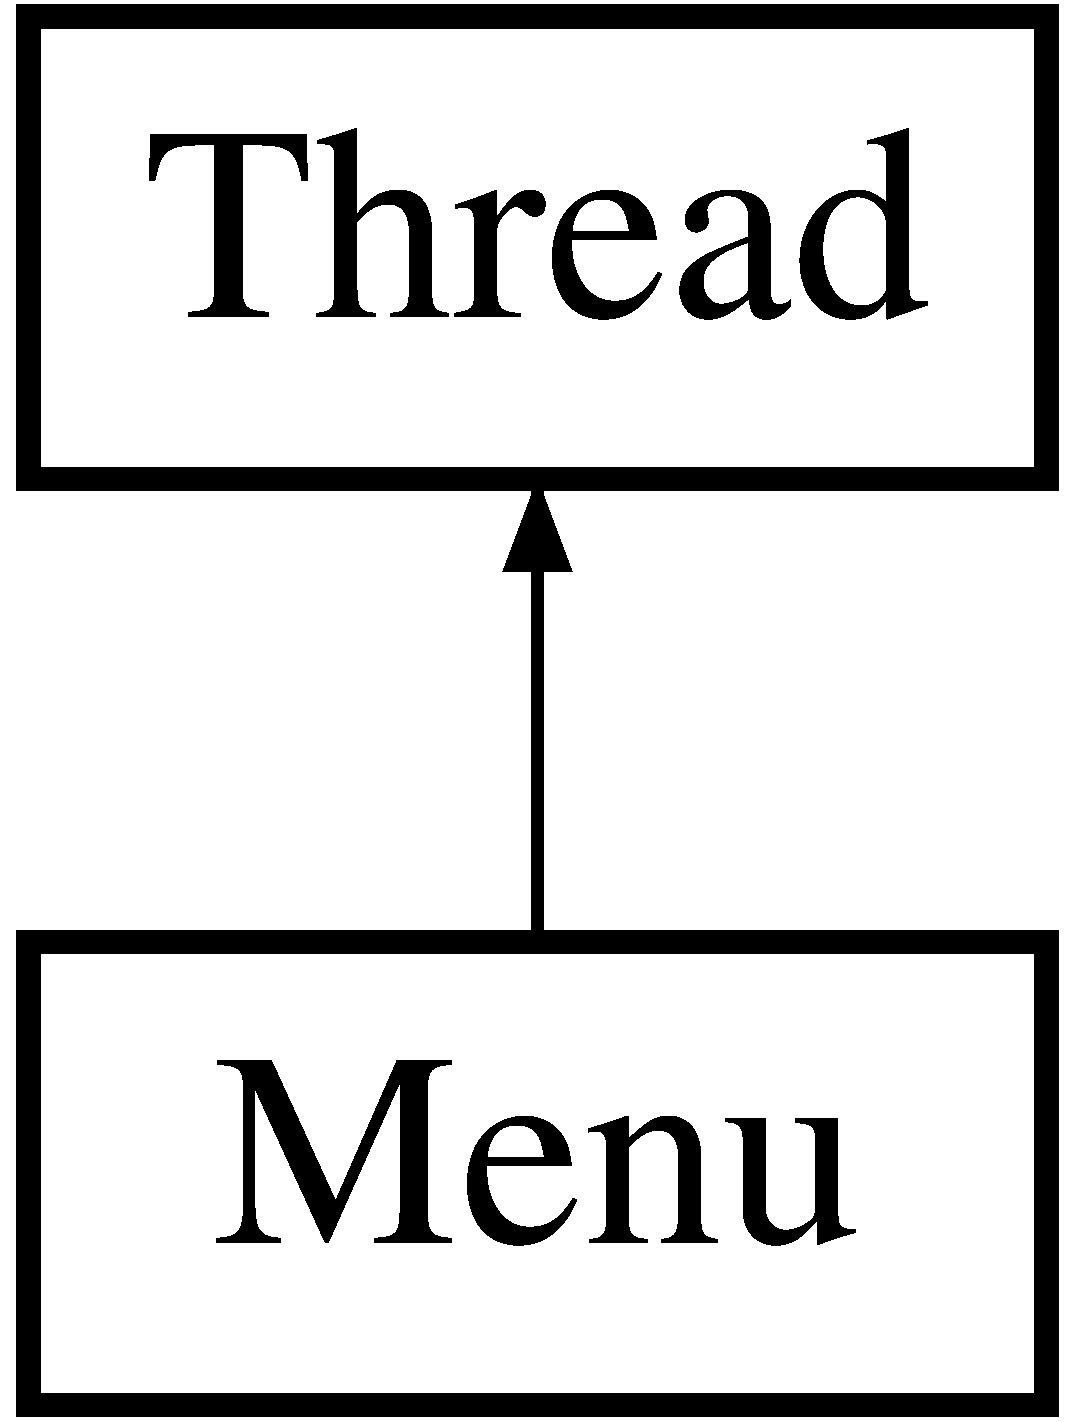
\includegraphics[height=2.000000cm]{class_menu_1_1_menu}
\end{center}
\end{figure}
\subsection*{Public Member Functions}
\begin{DoxyCompactItemize}
\item 
\mbox{\Hypertarget{class_menu_1_1_menu_ae64f0875afe3067b97ba370b354b9213}\label{class_menu_1_1_menu_ae64f0875afe3067b97ba370b354b9213}} 
def {\bfseries \+\_\+\+\_\+init\+\_\+\+\_\+} (self)
\item 
\mbox{\Hypertarget{class_menu_1_1_menu_a0b799a782ab40afc9aaa24bdab882113}\label{class_menu_1_1_menu_a0b799a782ab40afc9aaa24bdab882113}} 
def {\bfseries update\+\_\+mse} (self, mse)
\item 
def \mbox{\hyperlink{class_menu_1_1_menu_ac7d46e7da5b790d5efa729c03debbaf1}{update\+\_\+param}} (self, value, idx)
\item 
def \mbox{\hyperlink{class_menu_1_1_menu_ad22709b2e67308af35f55680d5a026e0}{run}} (self)
\item 
\mbox{\Hypertarget{class_menu_1_1_menu_adb7ed53932939535e6f6343644e6731a}\label{class_menu_1_1_menu_adb7ed53932939535e6f6343644e6731a}} 
def {\bfseries generate\+\_\+attacks\+\_\+panel} (self)
\item 
def \mbox{\hyperlink{class_menu_1_1_menu_a27ecebb6378a0b8dd1580f5fd1ba5c76}{freeze}} (self)
\item 
def \mbox{\hyperlink{class_menu_1_1_menu_a6a933e1b66dd2707e798efa5dbe724a7}{create\+\_\+fictive\+\_\+anchor}} (self)
\item 
def \mbox{\hyperlink{class_menu_1_1_menu_a47a07cce1b4c80a7d3c0a41045015f69}{create\+\_\+fictive\+\_\+tag}} (self)
\item 
def \mbox{\hyperlink{class_menu_1_1_menu_a32babc5b86a4f39290d2d4a10ef0ec5c}{display\+\_\+corrections}} (self)
\item 
\mbox{\Hypertarget{class_menu_1_1_menu_abd427cc12572cc5e157ab2ef25d1faf0}\label{class_menu_1_1_menu_abd427cc12572cc5e157ab2ef25d1faf0}} 
def {\bfseries show\+\_\+\+M\+SE} (self)
\item 
def \mbox{\hyperlink{class_menu_1_1_menu_a11923ed3ba9281c75035cbebc022fbf2}{simulate\+\_\+attack}} (self, target)
\item 
def \mbox{\hyperlink{class_menu_1_1_menu_a116637ec8c851d32fde26d0155337cbe}{space}} (self)
\item 
def \mbox{\hyperlink{class_menu_1_1_menu_ae075907d13c81100442befb9dd9c63c1}{callback}} (self)
\item 
def \mbox{\hyperlink{class_menu_1_1_menu_aabea3c091001d3cfad62483ffa367db8}{get\+Accel}} (self)
\item 
def \mbox{\hyperlink{class_menu_1_1_menu_a51829b63adb24ac48d350dee60181002}{reset}} (self)
\end{DoxyCompactItemize}
\subsection*{Data Fields}
\begin{DoxyCompactItemize}
\item 
\mbox{\Hypertarget{class_menu_1_1_menu_acec6d8ad52a28972fa74e071c1a63b6a}\label{class_menu_1_1_menu_acec6d8ad52a28972fa74e071c1a63b6a}} 
{\bfseries scale}
\item 
\mbox{\Hypertarget{class_menu_1_1_menu_a335628f2e9085305224b4f9cc6e95ed5}\label{class_menu_1_1_menu_a335628f2e9085305224b4f9cc6e95ed5}} 
{\bfseries var}
\item 
\mbox{\Hypertarget{class_menu_1_1_menu_a5423e5930789063b2687eb70d4e3194f}\label{class_menu_1_1_menu_a5423e5930789063b2687eb70d4e3194f}} 
{\bfseries accel}
\item 
\mbox{\Hypertarget{class_menu_1_1_menu_ae9a919d8e6f16d72b9d81aa3fd547670}\label{class_menu_1_1_menu_ae9a919d8e6f16d72b9d81aa3fd547670}} 
{\bfseries anchors\+\_\+list}
\item 
\mbox{\Hypertarget{class_menu_1_1_menu_a5b6e802d562adb1eb9a60ae8e8ca2ea0}\label{class_menu_1_1_menu_a5b6e802d562adb1eb9a60ae8e8ca2ea0}} 
{\bfseries tags\+\_\+list}
\item 
\mbox{\Hypertarget{class_menu_1_1_menu_ab8ed51749f1b4cff40604078a18fe9de}\label{class_menu_1_1_menu_ab8ed51749f1b4cff40604078a18fe9de}} 
{\bfseries attack\+\_\+list}
\item 
\mbox{\Hypertarget{class_menu_1_1_menu_a89791cf2c3bf608a399a70f0fb1e3d90}\label{class_menu_1_1_menu_a89791cf2c3bf608a399a70f0fb1e3d90}} 
{\bfseries attack\+\_\+offset}
\item 
\mbox{\Hypertarget{class_menu_1_1_menu_ab4b8daf4b8ea9d39568719e1e320076f}\label{class_menu_1_1_menu_ab4b8daf4b8ea9d39568719e1e320076f}} 
{\bfseries root}
\item 
\mbox{\Hypertarget{class_menu_1_1_menu_a906e5471892a6af403fcff0a3493a3ab}\label{class_menu_1_1_menu_a906e5471892a6af403fcff0a3493a3ab}} 
{\bfseries frozen}
\item 
\mbox{\Hypertarget{class_menu_1_1_menu_ae3588d6b8a60b8198aced11bfe3f2126}\label{class_menu_1_1_menu_ae3588d6b8a60b8198aced11bfe3f2126}} 
{\bfseries mse}
\item 
\mbox{\Hypertarget{class_menu_1_1_menu_a90cd8885aa787fbd5b97697ce259f3b6}\label{class_menu_1_1_menu_a90cd8885aa787fbd5b97697ce259f3b6}} 
{\bfseries hidden}
\item 
\mbox{\Hypertarget{class_menu_1_1_menu_a943f49763dd36e31fc7ea8604fcad789}\label{class_menu_1_1_menu_a943f49763dd36e31fc7ea8604fcad789}} 
{\bfseries frame}
\item 
\mbox{\Hypertarget{class_menu_1_1_menu_a00a9fca022b8c828786cf76ecaa05370}\label{class_menu_1_1_menu_a00a9fca022b8c828786cf76ecaa05370}} 
{\bfseries M\+SE}
\item 
\mbox{\Hypertarget{class_menu_1_1_menu_afa9e9838abb44338f7cbe41dc6f846d4}\label{class_menu_1_1_menu_afa9e9838abb44338f7cbe41dc6f846d4}} 
{\bfseries canvas}
\item 
\mbox{\Hypertarget{class_menu_1_1_menu_a03e73c7776db586ba8e288f6d62e3eb5}\label{class_menu_1_1_menu_a03e73c7776db586ba8e288f6d62e3eb5}} 
{\bfseries application\+\_\+pipe}
\item 
\mbox{\Hypertarget{class_menu_1_1_menu_ab777d6e803f79ff8e22244635dff6302}\label{class_menu_1_1_menu_ab777d6e803f79ff8e22244635dff6302}} 
\mbox{\hyperlink{class_menu_1_1_menu_ab777d6e803f79ff8e22244635dff6302}{fictive\+\_\+anchor\+\_\+x}}
\begin{DoxyCompactList}\small\item\em freeze button \end{DoxyCompactList}\item 
\mbox{\Hypertarget{class_menu_1_1_menu_a1a6ecb330d873834ad9959ae063a6057}\label{class_menu_1_1_menu_a1a6ecb330d873834ad9959ae063a6057}} 
{\bfseries fictive\+\_\+anchor\+\_\+y}
\item 
\mbox{\Hypertarget{class_menu_1_1_menu_a200fbb0edf63474dc68d8421b75112b5}\label{class_menu_1_1_menu_a200fbb0edf63474dc68d8421b75112b5}} 
{\bfseries fictive\+\_\+anchor\+\_\+z}
\item 
\mbox{\Hypertarget{class_menu_1_1_menu_a80225cc123ad5ae1b7a511922b7faf90}\label{class_menu_1_1_menu_a80225cc123ad5ae1b7a511922b7faf90}} 
{\bfseries fictive\+\_\+tag\+\_\+x}
\item 
\mbox{\Hypertarget{class_menu_1_1_menu_aed183ff5bb760cfe7585765fef279032}\label{class_menu_1_1_menu_aed183ff5bb760cfe7585765fef279032}} 
{\bfseries fictive\+\_\+tag\+\_\+y}
\item 
\mbox{\Hypertarget{class_menu_1_1_menu_af6ef9a398329eb25e434ad3399c21373}\label{class_menu_1_1_menu_af6ef9a398329eb25e434ad3399c21373}} 
{\bfseries fictive\+\_\+tag\+\_\+z}
\item 
\mbox{\Hypertarget{class_menu_1_1_menu_a564d49ff5a855daa8fec601111725599}\label{class_menu_1_1_menu_a564d49ff5a855daa8fec601111725599}} 
\mbox{\hyperlink{class_menu_1_1_menu_a564d49ff5a855daa8fec601111725599}{attacks}}
\begin{DoxyCompactList}\small\item\em attacks spinbox \end{DoxyCompactList}\item 
\mbox{\Hypertarget{class_menu_1_1_menu_a949decce69b0df45cc6faf9b2efdc51a}\label{class_menu_1_1_menu_a949decce69b0df45cc6faf9b2efdc51a}} 
{\bfseries attack\+\_\+spinbox}
\item 
\mbox{\Hypertarget{class_menu_1_1_menu_a4a461f6c5ec2ce0f28c3be0a1cf2d787}\label{class_menu_1_1_menu_a4a461f6c5ec2ce0f28c3be0a1cf2d787}} 
\mbox{\hyperlink{class_menu_1_1_menu_a4a461f6c5ec2ce0f28c3be0a1cf2d787}{attack\+\_\+offset\+\_\+label}}
\begin{DoxyCompactList}\small\item\em attacks offset entry \end{DoxyCompactList}\item 
\mbox{\Hypertarget{class_menu_1_1_menu_aa7f3ef1a3a73616aa12a5307dc9cc554}\label{class_menu_1_1_menu_aa7f3ef1a3a73616aa12a5307dc9cc554}} 
\mbox{\hyperlink{class_menu_1_1_menu_aa7f3ef1a3a73616aa12a5307dc9cc554}{anchors\+\_\+btns}}
\begin{DoxyCompactList}\small\item\em anchors buttons \end{DoxyCompactList}\item 
\mbox{\Hypertarget{class_menu_1_1_menu_a9335ed4e67e20e89e460be45f95af9c8}\label{class_menu_1_1_menu_a9335ed4e67e20e89e460be45f95af9c8}} 
\mbox{\hyperlink{class_menu_1_1_menu_a9335ed4e67e20e89e460be45f95af9c8}{tags\+\_\+btns}}
\begin{DoxyCompactList}\small\item\em tags buttons \end{DoxyCompactList}\end{DoxyCompactItemize}


\subsection{Detailed Description}
\begin{DoxyVerb}Interface for the localization engine control - triggers filtering & attack simulation\end{DoxyVerb}
 

\subsection{Member Function Documentation}
\mbox{\Hypertarget{class_menu_1_1_menu_ae075907d13c81100442befb9dd9c63c1}\label{class_menu_1_1_menu_ae075907d13c81100442befb9dd9c63c1}} 
\index{Menu\+::\+Menu@{Menu\+::\+Menu}!callback@{callback}}
\index{callback@{callback}!Menu\+::\+Menu@{Menu\+::\+Menu}}
\subsubsection{\texorpdfstring{callback()}{callback()}}
{\footnotesize\ttfamily def callback (\begin{DoxyParamCaption}\item[{}]{self }\end{DoxyParamCaption})}

\begin{DoxyVerb}Exit function\end{DoxyVerb}
 \mbox{\Hypertarget{class_menu_1_1_menu_a6a933e1b66dd2707e798efa5dbe724a7}\label{class_menu_1_1_menu_a6a933e1b66dd2707e798efa5dbe724a7}} 
\index{Menu\+::\+Menu@{Menu\+::\+Menu}!create\+\_\+fictive\+\_\+anchor@{create\+\_\+fictive\+\_\+anchor}}
\index{create\+\_\+fictive\+\_\+anchor@{create\+\_\+fictive\+\_\+anchor}!Menu\+::\+Menu@{Menu\+::\+Menu}}
\subsubsection{\texorpdfstring{create\+\_\+fictive\+\_\+anchor()}{create\_fictive\_anchor()}}
{\footnotesize\ttfamily def create\+\_\+fictive\+\_\+anchor (\begin{DoxyParamCaption}\item[{}]{self }\end{DoxyParamCaption})}

\begin{DoxyVerb}Creates an anchor at the given x,y,z coordinates\end{DoxyVerb}
 \mbox{\Hypertarget{class_menu_1_1_menu_a47a07cce1b4c80a7d3c0a41045015f69}\label{class_menu_1_1_menu_a47a07cce1b4c80a7d3c0a41045015f69}} 
\index{Menu\+::\+Menu@{Menu\+::\+Menu}!create\+\_\+fictive\+\_\+tag@{create\+\_\+fictive\+\_\+tag}}
\index{create\+\_\+fictive\+\_\+tag@{create\+\_\+fictive\+\_\+tag}!Menu\+::\+Menu@{Menu\+::\+Menu}}
\subsubsection{\texorpdfstring{create\+\_\+fictive\+\_\+tag()}{create\_fictive\_tag()}}
{\footnotesize\ttfamily def create\+\_\+fictive\+\_\+tag (\begin{DoxyParamCaption}\item[{}]{self }\end{DoxyParamCaption})}

\begin{DoxyVerb}Creates an tag at the given x,y,z coordinates\end{DoxyVerb}
 \mbox{\Hypertarget{class_menu_1_1_menu_a32babc5b86a4f39290d2d4a10ef0ec5c}\label{class_menu_1_1_menu_a32babc5b86a4f39290d2d4a10ef0ec5c}} 
\index{Menu\+::\+Menu@{Menu\+::\+Menu}!display\+\_\+corrections@{display\+\_\+corrections}}
\index{display\+\_\+corrections@{display\+\_\+corrections}!Menu\+::\+Menu@{Menu\+::\+Menu}}
\subsubsection{\texorpdfstring{display\+\_\+corrections()}{display\_corrections()}}
{\footnotesize\ttfamily def display\+\_\+corrections (\begin{DoxyParamCaption}\item[{}]{self }\end{DoxyParamCaption})}

\begin{DoxyVerb}Hide/display button for ranging correction scales\end{DoxyVerb}
 \mbox{\Hypertarget{class_menu_1_1_menu_a27ecebb6378a0b8dd1580f5fd1ba5c76}\label{class_menu_1_1_menu_a27ecebb6378a0b8dd1580f5fd1ba5c76}} 
\index{Menu\+::\+Menu@{Menu\+::\+Menu}!freeze@{freeze}}
\index{freeze@{freeze}!Menu\+::\+Menu@{Menu\+::\+Menu}}
\subsubsection{\texorpdfstring{freeze()}{freeze()}}
{\footnotesize\ttfamily def freeze (\begin{DoxyParamCaption}\item[{}]{self }\end{DoxyParamCaption})}

\begin{DoxyVerb}Freezes the execution in the 3D engine\end{DoxyVerb}
 \mbox{\Hypertarget{class_menu_1_1_menu_aabea3c091001d3cfad62483ffa367db8}\label{class_menu_1_1_menu_aabea3c091001d3cfad62483ffa367db8}} 
\index{Menu\+::\+Menu@{Menu\+::\+Menu}!get\+Accel@{get\+Accel}}
\index{get\+Accel@{get\+Accel}!Menu\+::\+Menu@{Menu\+::\+Menu}}
\subsubsection{\texorpdfstring{get\+Accel()}{getAccel()}}
{\footnotesize\ttfamily def get\+Accel (\begin{DoxyParamCaption}\item[{}]{self }\end{DoxyParamCaption})}

\begin{DoxyVerb}Returns acceleration\end{DoxyVerb}
 \mbox{\Hypertarget{class_menu_1_1_menu_a51829b63adb24ac48d350dee60181002}\label{class_menu_1_1_menu_a51829b63adb24ac48d350dee60181002}} 
\index{Menu\+::\+Menu@{Menu\+::\+Menu}!reset@{reset}}
\index{reset@{reset}!Menu\+::\+Menu@{Menu\+::\+Menu}}
\subsubsection{\texorpdfstring{reset()}{reset()}}
{\footnotesize\ttfamily def reset (\begin{DoxyParamCaption}\item[{}]{self }\end{DoxyParamCaption})}

\begin{DoxyVerb}Brings back correction scales to 0\end{DoxyVerb}
 \mbox{\Hypertarget{class_menu_1_1_menu_ad22709b2e67308af35f55680d5a026e0}\label{class_menu_1_1_menu_ad22709b2e67308af35f55680d5a026e0}} 
\index{Menu\+::\+Menu@{Menu\+::\+Menu}!run@{run}}
\index{run@{run}!Menu\+::\+Menu@{Menu\+::\+Menu}}
\subsubsection{\texorpdfstring{run()}{run()}}
{\footnotesize\ttfamily def run (\begin{DoxyParamCaption}\item[{}]{self }\end{DoxyParamCaption})}

\begin{DoxyVerb}Initializes Tkinter window, scales & buttons\end{DoxyVerb}
 \mbox{\Hypertarget{class_menu_1_1_menu_a11923ed3ba9281c75035cbebc022fbf2}\label{class_menu_1_1_menu_a11923ed3ba9281c75035cbebc022fbf2}} 
\index{Menu\+::\+Menu@{Menu\+::\+Menu}!simulate\+\_\+attack@{simulate\+\_\+attack}}
\index{simulate\+\_\+attack@{simulate\+\_\+attack}!Menu\+::\+Menu@{Menu\+::\+Menu}}
\subsubsection{\texorpdfstring{simulate\+\_\+attack()}{simulate\_attack()}}
{\footnotesize\ttfamily def simulate\+\_\+attack (\begin{DoxyParamCaption}\item[{}]{self,  }\item[{}]{target }\end{DoxyParamCaption})}

\begin{DoxyVerb}Simulates the chosen attack in the spinbox on the chosen target\end{DoxyVerb}
 \mbox{\Hypertarget{class_menu_1_1_menu_a116637ec8c851d32fde26d0155337cbe}\label{class_menu_1_1_menu_a116637ec8c851d32fde26d0155337cbe}} 
\index{Menu\+::\+Menu@{Menu\+::\+Menu}!space@{space}}
\index{space@{space}!Menu\+::\+Menu@{Menu\+::\+Menu}}
\subsubsection{\texorpdfstring{space()}{space()}}
{\footnotesize\ttfamily def space (\begin{DoxyParamCaption}\item[{}]{self }\end{DoxyParamCaption})}

\begin{DoxyVerb}draws a seperator\end{DoxyVerb}
 \mbox{\Hypertarget{class_menu_1_1_menu_ac7d46e7da5b790d5efa729c03debbaf1}\label{class_menu_1_1_menu_ac7d46e7da5b790d5efa729c03debbaf1}} 
\index{Menu\+::\+Menu@{Menu\+::\+Menu}!update\+\_\+param@{update\+\_\+param}}
\index{update\+\_\+param@{update\+\_\+param}!Menu\+::\+Menu@{Menu\+::\+Menu}}
\subsubsection{\texorpdfstring{update\+\_\+param()}{update\_param()}}
{\footnotesize\ttfamily def update\+\_\+param (\begin{DoxyParamCaption}\item[{}]{self,  }\item[{}]{value,  }\item[{}]{idx }\end{DoxyParamCaption})}

\begin{DoxyVerb}handler for rangings correction parameters updating\end{DoxyVerb}
 

The documentation for this class was generated from the following file\+:\begin{DoxyCompactItemize}
\item 
C\+:/\+Users/pestourb/\+Documents/\+Git\+Hub/\+Secure\+Loc/Menu.\+py\end{DoxyCompactItemize}

\hypertarget{classjson_structures_1_1metadata}{}\section{metadata Class Reference}
\label{classjson_structures_1_1metadata}\index{metadata@{metadata}}
\subsection*{Public Member Functions}
\begin{DoxyCompactItemize}
\item 
\mbox{\Hypertarget{classjson_structures_1_1metadata_a24cd6e55b96cd55c72425ed932cb6d29}\label{classjson_structures_1_1metadata_a24cd6e55b96cd55c72425ed932cb6d29}} 
def {\bfseries \+\_\+\+\_\+init\+\_\+\+\_\+} (self, tabfile=\textquotesingle{}anchors.\+tab\textquotesingle{}, comments=\textquotesingle{}\textquotesingle{})
\item 
def \mbox{\hyperlink{classjson_structures_1_1metadata_ad58622cada13d50f915c4e27ca4c711e}{dump\+\_\+tabfile}} (self)
\item 
def \mbox{\hyperlink{classjson_structures_1_1metadata_a68cc2498d25cf6670863c141957ac262}{export}} (self)
\end{DoxyCompactItemize}
\subsection*{Data Fields}
\begin{DoxyCompactItemize}
\item 
\mbox{\Hypertarget{classjson_structures_1_1metadata_a00f9a31137e6954973ab5676cf14f447}\label{classjson_structures_1_1metadata_a00f9a31137e6954973ab5676cf14f447}} 
{\bfseries tabfile}
\item 
\mbox{\Hypertarget{classjson_structures_1_1metadata_a5a5e3e8b4bd0d8acb4188aa82bce8786}\label{classjson_structures_1_1metadata_a5a5e3e8b4bd0d8acb4188aa82bce8786}} 
{\bfseries tabfile\+\_\+content}
\item 
\mbox{\Hypertarget{classjson_structures_1_1metadata_a64b8b36116751d566275b722e40bb3a7}\label{classjson_structures_1_1metadata_a64b8b36116751d566275b722e40bb3a7}} 
{\bfseries comments}
\end{DoxyCompactItemize}


\subsection{Detailed Description}
\begin{DoxyVerb}Contains information on the parameters used for measurements\end{DoxyVerb}
 

\subsection{Member Function Documentation}
\mbox{\Hypertarget{classjson_structures_1_1metadata_ad58622cada13d50f915c4e27ca4c711e}\label{classjson_structures_1_1metadata_ad58622cada13d50f915c4e27ca4c711e}} 
\index{json\+Structures\+::metadata@{json\+Structures\+::metadata}!dump\+\_\+tabfile@{dump\+\_\+tabfile}}
\index{dump\+\_\+tabfile@{dump\+\_\+tabfile}!json\+Structures\+::metadata@{json\+Structures\+::metadata}}
\subsubsection{\texorpdfstring{dump\+\_\+tabfile()}{dump\_tabfile()}}
{\footnotesize\ttfamily def dump\+\_\+tabfile (\begin{DoxyParamCaption}\item[{}]{self }\end{DoxyParamCaption})}

\begin{DoxyVerb}returns the content of anchors tabfile as a string\end{DoxyVerb}
 \mbox{\Hypertarget{classjson_structures_1_1metadata_a68cc2498d25cf6670863c141957ac262}\label{classjson_structures_1_1metadata_a68cc2498d25cf6670863c141957ac262}} 
\index{json\+Structures\+::metadata@{json\+Structures\+::metadata}!export@{export}}
\index{export@{export}!json\+Structures\+::metadata@{json\+Structures\+::metadata}}
\subsubsection{\texorpdfstring{export()}{export()}}
{\footnotesize\ttfamily def export (\begin{DoxyParamCaption}\item[{}]{self }\end{DoxyParamCaption})}

\begin{DoxyVerb}returns metadata as dictionary\end{DoxyVerb}
 

The documentation for this class was generated from the following file\+:\begin{DoxyCompactItemize}
\item 
C\+:/\+Users/pestourb/\+Documents/\+Git\+Hub/\+Secure\+Loc/json\+Structures.\+py\end{DoxyCompactItemize}

\hypertarget{class_emulator_1_1_motion_generator}{}\section{Motion\+Generator Class Reference}
\label{class_emulator_1_1_motion_generator}\index{Motion\+Generator@{Motion\+Generator}}
\subsection*{Public Member Functions}
\begin{DoxyCompactItemize}
\item 
\mbox{\Hypertarget{class_emulator_1_1_motion_generator_ae846cfa9ceebef5acb7e1b8ea109f55a}\label{class_emulator_1_1_motion_generator_ae846cfa9ceebef5acb7e1b8ea109f55a}} 
def {\bfseries generate\+\_\+random\+\_\+speed\+\_\+2D} (max\+\_\+speed=M\+A\+X\+\_\+\+S\+P\+E\+ED)
\end{DoxyCompactItemize}
\subsection*{Static Public Member Functions}
\begin{DoxyCompactItemize}
\item 
\mbox{\Hypertarget{class_emulator_1_1_motion_generator_a40d631f14f6e500846c5fe23835ec6a4}\label{class_emulator_1_1_motion_generator_a40d631f14f6e500846c5fe23835ec6a4}} 
def {\bfseries generate\+\_\+random\+\_\+speed} (max\+\_\+speed=M\+A\+X\+\_\+\+S\+P\+E\+ED)
\end{DoxyCompactItemize}


The documentation for this class was generated from the following file\+:\begin{DoxyCompactItemize}
\item 
C\+:/\+Users/pestourb/\+Documents/\+Git\+Hub/\+Secure\+Loc/Emulator.\+py\end{DoxyCompactItemize}

\hypertarget{classmovingentity_1_1_moving_entity}{}\section{Moving\+Entity Class Reference}
\label{classmovingentity_1_1_moving_entity}\index{Moving\+Entity@{Moving\+Entity}}
Inheritance diagram for Moving\+Entity\+:\begin{figure}[H]
\begin{center}
\leavevmode
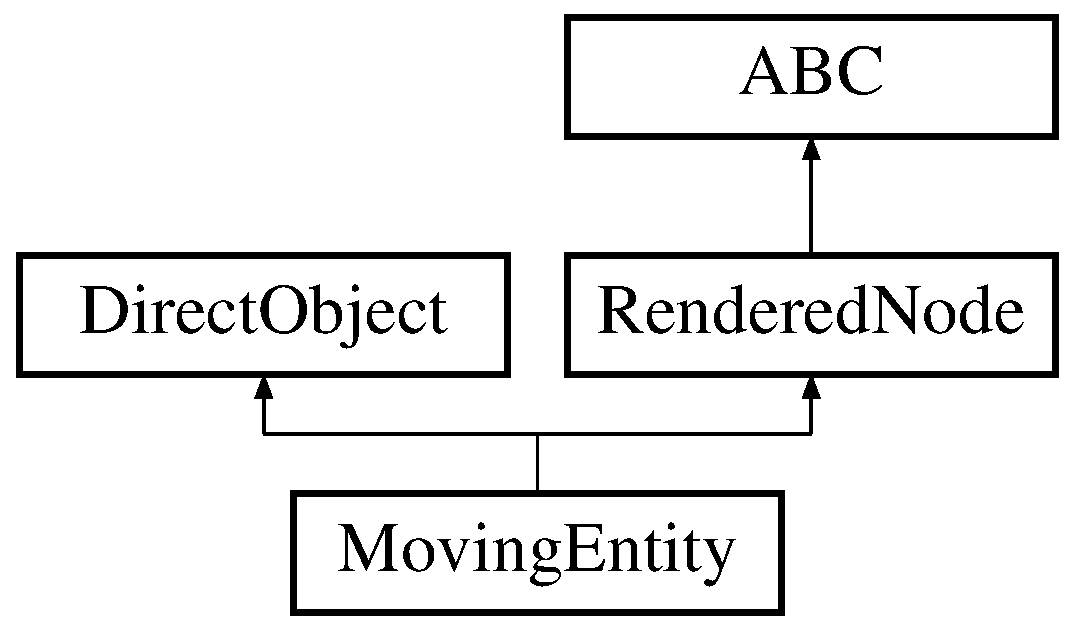
\includegraphics[height=3.000000cm]{classmovingentity_1_1_moving_entity}
\end{center}
\end{figure}
\subsection*{Public Member Functions}
\begin{DoxyCompactItemize}
\item 
\mbox{\Hypertarget{classmovingentity_1_1_moving_entity_a12b1c3f794a44ea527a3eafe82e0f8e8}\label{classmovingentity_1_1_moving_entity_a12b1c3f794a44ea527a3eafe82e0f8e8}} 
def {\bfseries \+\_\+\+\_\+init\+\_\+\+\_\+} (self, name, color=\textquotesingle{}orange\textquotesingle{})
\item 
\mbox{\Hypertarget{classmovingentity_1_1_moving_entity_a89c968c83617e2fca6e64e74c6478b58}\label{classmovingentity_1_1_moving_entity_a89c968c83617e2fca6e64e74c6478b58}} 
def {\bfseries get\+\_\+coordinates} (self)
\item 
def \mbox{\hyperlink{classmovingentity_1_1_moving_entity_afc59fd77ac0d0375226e77947f7f6624}{set\+\_\+coordinates}} (self, x, y, z)
\item 
def \mbox{\hyperlink{classmovingentity_1_1_moving_entity_a09f3f97175c16ea6025da871f653d416}{get\+\_\+\+ID}} (self)
\item 
def \mbox{\hyperlink{classmovingentity_1_1_moving_entity_a8497086c897585b6ee2234e8728e69e5}{get\+\_\+all\+\_\+distances}} (self)
\item 
def \mbox{\hyperlink{classmovingentity_1_1_moving_entity_a5b39ecfe3f50dcace4ea880ef22db24d}{get\+\_\+discretized\+\_\+coordinates}} (self, x, y, z, granularity=S\+Q\+U\+A\+R\+E\+\_\+\+S\+I\+ZE)
\item 
def \mbox{\hyperlink{classmovingentity_1_1_moving_entity_a2d32bac446feb8ad06df10e2af16f595}{get\+\_\+current\+\_\+pos}} (self)
\item 
def \mbox{\hyperlink{classmovingentity_1_1_moving_entity_a601e216b9aab14b2fb91b50b3af9db2d}{get\+\_\+previous\+\_\+pos}} (self)
\item 
def \mbox{\hyperlink{classmovingentity_1_1_moving_entity_a17e5bc839e5dae9b73b8454fed5c216c}{get\+\_\+position}} (self)
\item 
def \mbox{\hyperlink{classmovingentity_1_1_moving_entity_a8c0cf2c98dee238d1694be0a9ac45d1c}{set\+\_\+position}} (self, pos)
\item 
def \mbox{\hyperlink{classmovingentity_1_1_moving_entity_a822153dd41281662677b57fb6dbdb0a0}{get\+\_\+abs\+\_\+speed}} (self)
\item 
def \mbox{\hyperlink{classmovingentity_1_1_moving_entity_a6bad37eefcaed99163217d58444c2624}{get\+\_\+abs\+\_\+acc}} (self)
\item 
def \mbox{\hyperlink{classmovingentity_1_1_moving_entity_a86f9b2b879ff5e2db1010bdf4d5a03a1}{set\+\_\+speed\+\_\+vector}} (self, speed\+\_\+vector, replace\+\_\+last=False)
\item 
def \mbox{\hyperlink{classmovingentity_1_1_moving_entity_a42416d83ae7a1df561c13585f1389a6e}{set\+\_\+acc\+\_\+vector}} (self, acc, replace\+\_\+last=False)
\item 
def \mbox{\hyperlink{classmovingentity_1_1_moving_entity_a6e456d51469dc3f6d79559a1c0a552b5}{get\+\_\+speed\+\_\+vector}} (self)
\item 
def \mbox{\hyperlink{classmovingentity_1_1_moving_entity_ac53c8044d0401c60c3a6070cf22caee8}{get\+\_\+acc\+\_\+vector}} (self)
\item 
def \mbox{\hyperlink{classmovingentity_1_1_moving_entity_a547093d75e0e1ade6c2df927e0907bd6}{compute\+\_\+speed}} (self, replace\+\_\+mode=False)
\item 
def \mbox{\hyperlink{classmovingentity_1_1_moving_entity_a799b068567d0358b6bc0f6ec2cbdeb02}{compute\+\_\+acc}} (self, replace\+\_\+mode=False)
\end{DoxyCompactItemize}
\subsection*{Data Fields}
\begin{DoxyCompactItemize}
\item 
\mbox{\Hypertarget{classmovingentity_1_1_moving_entity_ab74e6bf80237ddc4109968cedc58c151}\label{classmovingentity_1_1_moving_entity_ab74e6bf80237ddc4109968cedc58c151}} 
{\bfseries name}
\item 
\mbox{\Hypertarget{classmovingentity_1_1_moving_entity_ac17d0e3d420545b0cbe7c718cf026ddc}\label{classmovingentity_1_1_moving_entity_ac17d0e3d420545b0cbe7c718cf026ddc}} 
{\bfseries positions}
\item 
\mbox{\Hypertarget{classmovingentity_1_1_moving_entity_a69dc6ef2269f17b85dfb95fffad29d9f}\label{classmovingentity_1_1_moving_entity_a69dc6ef2269f17b85dfb95fffad29d9f}} 
{\bfseries speed\+\_\+vector}
\item 
\mbox{\Hypertarget{classmovingentity_1_1_moving_entity_a0b7c4c1c91c90593e9c359a6cbed6274}\label{classmovingentity_1_1_moving_entity_a0b7c4c1c91c90593e9c359a6cbed6274}} 
{\bfseries acc\+\_\+vector}
\item 
\mbox{\Hypertarget{classmovingentity_1_1_moving_entity_a37dbdc30935031c05304482e1be89d8f}\label{classmovingentity_1_1_moving_entity_a37dbdc30935031c05304482e1be89d8f}} 
{\bfseries color}
\item 
\mbox{\Hypertarget{classmovingentity_1_1_moving_entity_ab0db378e6ced1decdb42263d4cb2789a}\label{classmovingentity_1_1_moving_entity_ab0db378e6ced1decdb42263d4cb2789a}} 
{\bfseries ready}
\item 
\mbox{\Hypertarget{classmovingentity_1_1_moving_entity_ac6c1eeb684483c821de0ec90f6c47cb9}\label{classmovingentity_1_1_moving_entity_ac6c1eeb684483c821de0ec90f6c47cb9}} 
{\bfseries shown}
\end{DoxyCompactItemize}


\subsection{Detailed Description}
\begin{DoxyVerb}Moving tags\end{DoxyVerb}
 

\subsection{Member Function Documentation}
\mbox{\Hypertarget{classmovingentity_1_1_moving_entity_a799b068567d0358b6bc0f6ec2cbdeb02}\label{classmovingentity_1_1_moving_entity_a799b068567d0358b6bc0f6ec2cbdeb02}} 
\index{movingentity\+::\+Moving\+Entity@{movingentity\+::\+Moving\+Entity}!compute\+\_\+acc@{compute\+\_\+acc}}
\index{compute\+\_\+acc@{compute\+\_\+acc}!movingentity\+::\+Moving\+Entity@{movingentity\+::\+Moving\+Entity}}
\subsubsection{\texorpdfstring{compute\+\_\+acc()}{compute\_acc()}}
{\footnotesize\ttfamily def compute\+\_\+acc (\begin{DoxyParamCaption}\item[{}]{self,  }\item[{}]{replace\+\_\+mode = {\ttfamily False} }\end{DoxyParamCaption})}

\begin{DoxyVerb}calculates the acceleration after each position update\end{DoxyVerb}
 \mbox{\Hypertarget{classmovingentity_1_1_moving_entity_a547093d75e0e1ade6c2df927e0907bd6}\label{classmovingentity_1_1_moving_entity_a547093d75e0e1ade6c2df927e0907bd6}} 
\index{movingentity\+::\+Moving\+Entity@{movingentity\+::\+Moving\+Entity}!compute\+\_\+speed@{compute\+\_\+speed}}
\index{compute\+\_\+speed@{compute\+\_\+speed}!movingentity\+::\+Moving\+Entity@{movingentity\+::\+Moving\+Entity}}
\subsubsection{\texorpdfstring{compute\+\_\+speed()}{compute\_speed()}}
{\footnotesize\ttfamily def compute\+\_\+speed (\begin{DoxyParamCaption}\item[{}]{self,  }\item[{}]{replace\+\_\+mode = {\ttfamily False} }\end{DoxyParamCaption})}

\begin{DoxyVerb}calculates the speed after each position update\end{DoxyVerb}
 \mbox{\Hypertarget{classmovingentity_1_1_moving_entity_a6bad37eefcaed99163217d58444c2624}\label{classmovingentity_1_1_moving_entity_a6bad37eefcaed99163217d58444c2624}} 
\index{movingentity\+::\+Moving\+Entity@{movingentity\+::\+Moving\+Entity}!get\+\_\+abs\+\_\+acc@{get\+\_\+abs\+\_\+acc}}
\index{get\+\_\+abs\+\_\+acc@{get\+\_\+abs\+\_\+acc}!movingentity\+::\+Moving\+Entity@{movingentity\+::\+Moving\+Entity}}
\subsubsection{\texorpdfstring{get\+\_\+abs\+\_\+acc()}{get\_abs\_acc()}}
{\footnotesize\ttfamily def get\+\_\+abs\+\_\+acc (\begin{DoxyParamCaption}\item[{}]{self }\end{DoxyParamCaption})}

\begin{DoxyVerb}computes the absolute acceleration from the acceleration vector\end{DoxyVerb}
 \mbox{\Hypertarget{classmovingentity_1_1_moving_entity_a822153dd41281662677b57fb6dbdb0a0}\label{classmovingentity_1_1_moving_entity_a822153dd41281662677b57fb6dbdb0a0}} 
\index{movingentity\+::\+Moving\+Entity@{movingentity\+::\+Moving\+Entity}!get\+\_\+abs\+\_\+speed@{get\+\_\+abs\+\_\+speed}}
\index{get\+\_\+abs\+\_\+speed@{get\+\_\+abs\+\_\+speed}!movingentity\+::\+Moving\+Entity@{movingentity\+::\+Moving\+Entity}}
\subsubsection{\texorpdfstring{get\+\_\+abs\+\_\+speed()}{get\_abs\_speed()}}
{\footnotesize\ttfamily def get\+\_\+abs\+\_\+speed (\begin{DoxyParamCaption}\item[{}]{self }\end{DoxyParamCaption})}

\begin{DoxyVerb}computes the absolute speed from the speed vector\end{DoxyVerb}
 \mbox{\Hypertarget{classmovingentity_1_1_moving_entity_ac53c8044d0401c60c3a6070cf22caee8}\label{classmovingentity_1_1_moving_entity_ac53c8044d0401c60c3a6070cf22caee8}} 
\index{movingentity\+::\+Moving\+Entity@{movingentity\+::\+Moving\+Entity}!get\+\_\+acc\+\_\+vector@{get\+\_\+acc\+\_\+vector}}
\index{get\+\_\+acc\+\_\+vector@{get\+\_\+acc\+\_\+vector}!movingentity\+::\+Moving\+Entity@{movingentity\+::\+Moving\+Entity}}
\subsubsection{\texorpdfstring{get\+\_\+acc\+\_\+vector()}{get\_acc\_vector()}}
{\footnotesize\ttfamily def get\+\_\+acc\+\_\+vector (\begin{DoxyParamCaption}\item[{}]{self }\end{DoxyParamCaption})}

\begin{DoxyVerb}returns the most recent acceleration vector in the acceleration vector list\end{DoxyVerb}
 \mbox{\Hypertarget{classmovingentity_1_1_moving_entity_a8497086c897585b6ee2234e8728e69e5}\label{classmovingentity_1_1_moving_entity_a8497086c897585b6ee2234e8728e69e5}} 
\index{movingentity\+::\+Moving\+Entity@{movingentity\+::\+Moving\+Entity}!get\+\_\+all\+\_\+distances@{get\+\_\+all\+\_\+distances}}
\index{get\+\_\+all\+\_\+distances@{get\+\_\+all\+\_\+distances}!movingentity\+::\+Moving\+Entity@{movingentity\+::\+Moving\+Entity}}
\subsubsection{\texorpdfstring{get\+\_\+all\+\_\+distances()}{get\_all\_distances()}}
{\footnotesize\ttfamily def get\+\_\+all\+\_\+distances (\begin{DoxyParamCaption}\item[{}]{self }\end{DoxyParamCaption})}

\begin{DoxyVerb}return the distances of the anchor with every robot as a dictionary.\end{DoxyVerb}
 \mbox{\Hypertarget{classmovingentity_1_1_moving_entity_a2d32bac446feb8ad06df10e2af16f595}\label{classmovingentity_1_1_moving_entity_a2d32bac446feb8ad06df10e2af16f595}} 
\index{movingentity\+::\+Moving\+Entity@{movingentity\+::\+Moving\+Entity}!get\+\_\+current\+\_\+pos@{get\+\_\+current\+\_\+pos}}
\index{get\+\_\+current\+\_\+pos@{get\+\_\+current\+\_\+pos}!movingentity\+::\+Moving\+Entity@{movingentity\+::\+Moving\+Entity}}
\subsubsection{\texorpdfstring{get\+\_\+current\+\_\+pos()}{get\_current\_pos()}}
{\footnotesize\ttfamily def get\+\_\+current\+\_\+pos (\begin{DoxyParamCaption}\item[{}]{self }\end{DoxyParamCaption})}

\begin{DoxyVerb}returns the most recent position in the position list\end{DoxyVerb}
 \mbox{\Hypertarget{classmovingentity_1_1_moving_entity_a5b39ecfe3f50dcace4ea880ef22db24d}\label{classmovingentity_1_1_moving_entity_a5b39ecfe3f50dcace4ea880ef22db24d}} 
\index{movingentity\+::\+Moving\+Entity@{movingentity\+::\+Moving\+Entity}!get\+\_\+discretized\+\_\+coordinates@{get\+\_\+discretized\+\_\+coordinates}}
\index{get\+\_\+discretized\+\_\+coordinates@{get\+\_\+discretized\+\_\+coordinates}!movingentity\+::\+Moving\+Entity@{movingentity\+::\+Moving\+Entity}}
\subsubsection{\texorpdfstring{get\+\_\+discretized\+\_\+coordinates()}{get\_discretized\_coordinates()}}
{\footnotesize\ttfamily def get\+\_\+discretized\+\_\+coordinates (\begin{DoxyParamCaption}\item[{}]{self,  }\item[{}]{x,  }\item[{}]{y,  }\item[{}]{z,  }\item[{}]{granularity = {\ttfamily SQUARE\+\_\+SIZE} }\end{DoxyParamCaption})}

\begin{DoxyVerb}returns the coordinates of the robot on a tiled floor.
Granularity is defined as the length of a tile\end{DoxyVerb}
 \mbox{\Hypertarget{classmovingentity_1_1_moving_entity_a09f3f97175c16ea6025da871f653d416}\label{classmovingentity_1_1_moving_entity_a09f3f97175c16ea6025da871f653d416}} 
\index{movingentity\+::\+Moving\+Entity@{movingentity\+::\+Moving\+Entity}!get\+\_\+\+ID@{get\+\_\+\+ID}}
\index{get\+\_\+\+ID@{get\+\_\+\+ID}!movingentity\+::\+Moving\+Entity@{movingentity\+::\+Moving\+Entity}}
\subsubsection{\texorpdfstring{get\+\_\+\+I\+D()}{get\_ID()}}
{\footnotesize\ttfamily def get\+\_\+\+ID (\begin{DoxyParamCaption}\item[{}]{self }\end{DoxyParamCaption})}

\begin{DoxyVerb}returns tag ID\end{DoxyVerb}
 \mbox{\Hypertarget{classmovingentity_1_1_moving_entity_a17e5bc839e5dae9b73b8454fed5c216c}\label{classmovingentity_1_1_moving_entity_a17e5bc839e5dae9b73b8454fed5c216c}} 
\index{movingentity\+::\+Moving\+Entity@{movingentity\+::\+Moving\+Entity}!get\+\_\+position@{get\+\_\+position}}
\index{get\+\_\+position@{get\+\_\+position}!movingentity\+::\+Moving\+Entity@{movingentity\+::\+Moving\+Entity}}
\subsubsection{\texorpdfstring{get\+\_\+position()}{get\_position()}}
{\footnotesize\ttfamily def get\+\_\+position (\begin{DoxyParamCaption}\item[{}]{self }\end{DoxyParamCaption})}

\begin{DoxyVerb}Calls get_coordinates\end{DoxyVerb}
 \mbox{\Hypertarget{classmovingentity_1_1_moving_entity_a601e216b9aab14b2fb91b50b3af9db2d}\label{classmovingentity_1_1_moving_entity_a601e216b9aab14b2fb91b50b3af9db2d}} 
\index{movingentity\+::\+Moving\+Entity@{movingentity\+::\+Moving\+Entity}!get\+\_\+previous\+\_\+pos@{get\+\_\+previous\+\_\+pos}}
\index{get\+\_\+previous\+\_\+pos@{get\+\_\+previous\+\_\+pos}!movingentity\+::\+Moving\+Entity@{movingentity\+::\+Moving\+Entity}}
\subsubsection{\texorpdfstring{get\+\_\+previous\+\_\+pos()}{get\_previous\_pos()}}
{\footnotesize\ttfamily def get\+\_\+previous\+\_\+pos (\begin{DoxyParamCaption}\item[{}]{self }\end{DoxyParamCaption})}

\begin{DoxyVerb}returns previous position for speed calculation\end{DoxyVerb}
 \mbox{\Hypertarget{classmovingentity_1_1_moving_entity_a6e456d51469dc3f6d79559a1c0a552b5}\label{classmovingentity_1_1_moving_entity_a6e456d51469dc3f6d79559a1c0a552b5}} 
\index{movingentity\+::\+Moving\+Entity@{movingentity\+::\+Moving\+Entity}!get\+\_\+speed\+\_\+vector@{get\+\_\+speed\+\_\+vector}}
\index{get\+\_\+speed\+\_\+vector@{get\+\_\+speed\+\_\+vector}!movingentity\+::\+Moving\+Entity@{movingentity\+::\+Moving\+Entity}}
\subsubsection{\texorpdfstring{get\+\_\+speed\+\_\+vector()}{get\_speed\_vector()}}
{\footnotesize\ttfamily def get\+\_\+speed\+\_\+vector (\begin{DoxyParamCaption}\item[{}]{self }\end{DoxyParamCaption})}

\begin{DoxyVerb}returns the most recent speed vector in the speed vector list\end{DoxyVerb}
 \mbox{\Hypertarget{classmovingentity_1_1_moving_entity_a42416d83ae7a1df561c13585f1389a6e}\label{classmovingentity_1_1_moving_entity_a42416d83ae7a1df561c13585f1389a6e}} 
\index{movingentity\+::\+Moving\+Entity@{movingentity\+::\+Moving\+Entity}!set\+\_\+acc\+\_\+vector@{set\+\_\+acc\+\_\+vector}}
\index{set\+\_\+acc\+\_\+vector@{set\+\_\+acc\+\_\+vector}!movingentity\+::\+Moving\+Entity@{movingentity\+::\+Moving\+Entity}}
\subsubsection{\texorpdfstring{set\+\_\+acc\+\_\+vector()}{set\_acc\_vector()}}
{\footnotesize\ttfamily def set\+\_\+acc\+\_\+vector (\begin{DoxyParamCaption}\item[{}]{self,  }\item[{}]{acc,  }\item[{}]{replace\+\_\+last = {\ttfamily False} }\end{DoxyParamCaption})}

\begin{DoxyVerb}Appends current acceleration to acceleration list and removes the oldes acceleration data stored\end{DoxyVerb}
 \mbox{\Hypertarget{classmovingentity_1_1_moving_entity_afc59fd77ac0d0375226e77947f7f6624}\label{classmovingentity_1_1_moving_entity_afc59fd77ac0d0375226e77947f7f6624}} 
\index{movingentity\+::\+Moving\+Entity@{movingentity\+::\+Moving\+Entity}!set\+\_\+coordinates@{set\+\_\+coordinates}}
\index{set\+\_\+coordinates@{set\+\_\+coordinates}!movingentity\+::\+Moving\+Entity@{movingentity\+::\+Moving\+Entity}}
\subsubsection{\texorpdfstring{set\+\_\+coordinates()}{set\_coordinates()}}
{\footnotesize\ttfamily def set\+\_\+coordinates (\begin{DoxyParamCaption}\item[{}]{self,  }\item[{}]{x,  }\item[{}]{y,  }\item[{}]{z }\end{DoxyParamCaption})}

\begin{DoxyVerb}Sets the tag coordinates. Should be used carefully; this will lead to errors in the localization algorithm.
Use move_node instead if you wish to move only the node representation in the 3D engine\end{DoxyVerb}
 \mbox{\Hypertarget{classmovingentity_1_1_moving_entity_a8c0cf2c98dee238d1694be0a9ac45d1c}\label{classmovingentity_1_1_moving_entity_a8c0cf2c98dee238d1694be0a9ac45d1c}} 
\index{movingentity\+::\+Moving\+Entity@{movingentity\+::\+Moving\+Entity}!set\+\_\+position@{set\+\_\+position}}
\index{set\+\_\+position@{set\+\_\+position}!movingentity\+::\+Moving\+Entity@{movingentity\+::\+Moving\+Entity}}
\subsubsection{\texorpdfstring{set\+\_\+position()}{set\_position()}}
{\footnotesize\ttfamily def set\+\_\+position (\begin{DoxyParamCaption}\item[{}]{self,  }\item[{}]{pos }\end{DoxyParamCaption})}

\begin{DoxyVerb}Takes position as a tuple in input.
Sets coordinates and displays the node at its new position in the 3D engine\end{DoxyVerb}
 \mbox{\Hypertarget{classmovingentity_1_1_moving_entity_a86f9b2b879ff5e2db1010bdf4d5a03a1}\label{classmovingentity_1_1_moving_entity_a86f9b2b879ff5e2db1010bdf4d5a03a1}} 
\index{movingentity\+::\+Moving\+Entity@{movingentity\+::\+Moving\+Entity}!set\+\_\+speed\+\_\+vector@{set\+\_\+speed\+\_\+vector}}
\index{set\+\_\+speed\+\_\+vector@{set\+\_\+speed\+\_\+vector}!movingentity\+::\+Moving\+Entity@{movingentity\+::\+Moving\+Entity}}
\subsubsection{\texorpdfstring{set\+\_\+speed\+\_\+vector()}{set\_speed\_vector()}}
{\footnotesize\ttfamily def set\+\_\+speed\+\_\+vector (\begin{DoxyParamCaption}\item[{}]{self,  }\item[{}]{speed\+\_\+vector,  }\item[{}]{replace\+\_\+last = {\ttfamily False} }\end{DoxyParamCaption})}

\begin{DoxyVerb}Appends current speed to speed list and
removes the oldest speed data stored\end{DoxyVerb}
 

The documentation for this class was generated from the following file\+:\begin{DoxyCompactItemize}
\item 
C\+:/\+Users/pestourb/\+Documents/\+Git\+Hub/\+Secure\+Loc/movingentity.\+py\end{DoxyCompactItemize}

\hypertarget{class_emulator_1_1_node}{}\section{Node Class Reference}
\label{class_emulator_1_1_node}\index{Node@{Node}}
Inheritance diagram for Node\+:\begin{figure}[H]
\begin{center}
\leavevmode
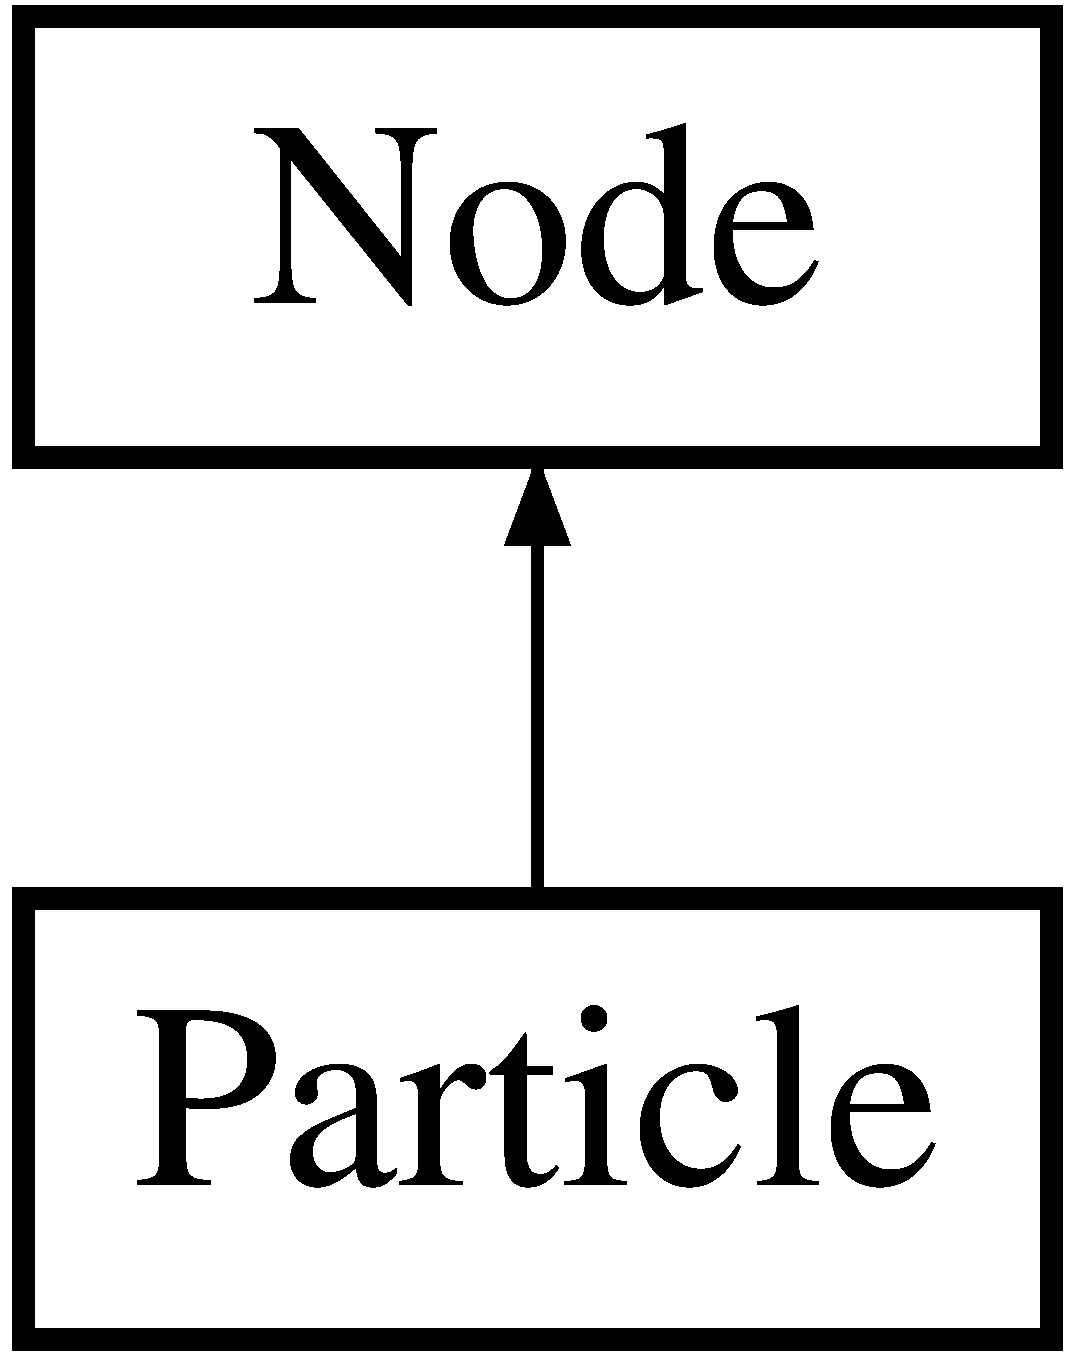
\includegraphics[height=2.000000cm]{class_emulator_1_1_node}
\end{center}
\end{figure}
\subsection*{Public Member Functions}
\begin{DoxyCompactItemize}
\item 
\mbox{\Hypertarget{class_emulator_1_1_node_ac43dc993c13bff5b6c6b607b6029b627}\label{class_emulator_1_1_node_ac43dc993c13bff5b6c6b607b6029b627}} 
def {\bfseries \+\_\+\+\_\+init\+\_\+\+\_\+} (self, x, y, z, name=\textquotesingle{}Anonymous\textquotesingle{}, is\+\_\+ref=False)
\item 
\mbox{\Hypertarget{class_emulator_1_1_node_a4c8b8381ab3d5ec726c1ac0a605b0cc1}\label{class_emulator_1_1_node_a4c8b8381ab3d5ec726c1ac0a605b0cc1}} 
def {\bfseries get\+\_\+distance\+\_\+to\+\_\+pos} (self, pos)
\item 
\mbox{\Hypertarget{class_emulator_1_1_node_a029192a087701ed05b647b566687054e}\label{class_emulator_1_1_node_a029192a087701ed05b647b566687054e}} 
def {\bfseries get\+\_\+distance} (self, node)
\item 
\mbox{\Hypertarget{class_emulator_1_1_node_ac1c282ef457c86e57f059d889fd109a6}\label{class_emulator_1_1_node_ac1c282ef457c86e57f059d889fd109a6}} 
def {\bfseries get\+\_\+distance\+\_\+noisy} (self, pos)
\item 
\mbox{\Hypertarget{class_emulator_1_1_node_ac678816339dde4c5fd312b183fbef3c7}\label{class_emulator_1_1_node_ac678816339dde4c5fd312b183fbef3c7}} 
def {\bfseries generate\+\_\+noise} (self)
\item 
\mbox{\Hypertarget{class_emulator_1_1_node_a914802152a6586315fd4e22dd7131f88}\label{class_emulator_1_1_node_a914802152a6586315fd4e22dd7131f88}} 
def {\bfseries get\+\_\+pos} (self)
\item 
\mbox{\Hypertarget{class_emulator_1_1_node_af452979cc7ef897f3f022c542979fd3a}\label{class_emulator_1_1_node_af452979cc7ef897f3f022c542979fd3a}} 
def {\bfseries move} (self, pos)
\end{DoxyCompactItemize}
\subsection*{Data Fields}
\begin{DoxyCompactItemize}
\item 
\mbox{\Hypertarget{class_emulator_1_1_node_a9336ebf25087d91c818ee6e9ec29f8c1}\label{class_emulator_1_1_node_a9336ebf25087d91c818ee6e9ec29f8c1}} 
{\bfseries x}
\item 
\mbox{\Hypertarget{class_emulator_1_1_node_a2fb1c5cf58867b5bbc9a1b145a86f3a0}\label{class_emulator_1_1_node_a2fb1c5cf58867b5bbc9a1b145a86f3a0}} 
{\bfseries y}
\item 
\mbox{\Hypertarget{class_emulator_1_1_node_a25ed1bcb423b0b7200f485fc5ff71c8e}\label{class_emulator_1_1_node_a25ed1bcb423b0b7200f485fc5ff71c8e}} 
{\bfseries z}
\item 
\mbox{\Hypertarget{class_emulator_1_1_node_ab74e6bf80237ddc4109968cedc58c151}\label{class_emulator_1_1_node_ab74e6bf80237ddc4109968cedc58c151}} 
{\bfseries name}
\item 
\mbox{\Hypertarget{class_emulator_1_1_node_af24398adc3c93eab7c7458dd6d628a8e}\label{class_emulator_1_1_node_af24398adc3c93eab7c7458dd6d628a8e}} 
{\bfseries is\+\_\+ref}
\item 
\mbox{\Hypertarget{class_emulator_1_1_node_a5f275402fe7e3f672eab8b802e8913ca}\label{class_emulator_1_1_node_a5f275402fe7e3f672eab8b802e8913ca}} 
{\bfseries noise}
\end{DoxyCompactItemize}


The documentation for this class was generated from the following file\+:\begin{DoxyCompactItemize}
\item 
C\+:/\+Users/pestourb/\+Documents/\+Git\+Hub/\+Secure\+Loc/Emulator.\+py\end{DoxyCompactItemize}

\hypertarget{class_test_menu_1_1_page_one}{}\section{Page\+One Class Reference}
\label{class_test_menu_1_1_page_one}\index{Page\+One@{Page\+One}}
Inheritance diagram for Page\+One\+:\begin{figure}[H]
\begin{center}
\leavevmode
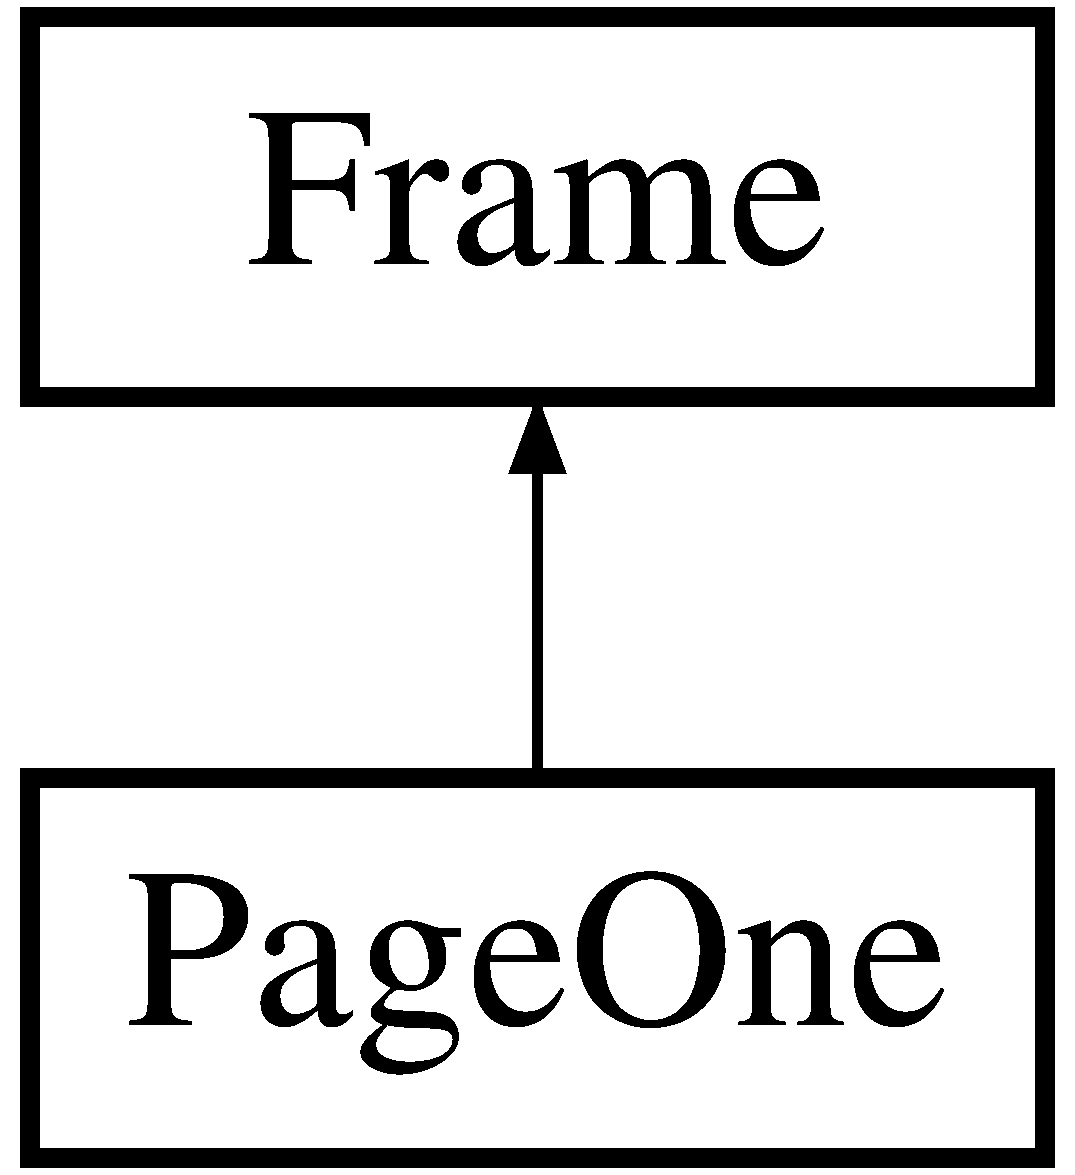
\includegraphics[height=2.000000cm]{class_test_menu_1_1_page_one}
\end{center}
\end{figure}
\subsection*{Public Member Functions}
\begin{DoxyCompactItemize}
\item 
\mbox{\Hypertarget{class_test_menu_1_1_page_one_a558d9afc290e8d1ff922f46114f16631}\label{class_test_menu_1_1_page_one_a558d9afc290e8d1ff922f46114f16631}} 
def {\bfseries \+\_\+\+\_\+init\+\_\+\+\_\+} (self, parent, controller)
\end{DoxyCompactItemize}


The documentation for this class was generated from the following file\+:\begin{DoxyCompactItemize}
\item 
C\+:/\+Users/pestourb/\+Documents/\+Git\+Hub/\+Secure\+Loc/Test\+Menu.\+py\end{DoxyCompactItemize}

\hypertarget{class_test_menu_1_1_page_three}{}\section{Page\+Three Class Reference}
\label{class_test_menu_1_1_page_three}\index{Page\+Three@{Page\+Three}}
Inheritance diagram for Page\+Three\+:\begin{figure}[H]
\begin{center}
\leavevmode
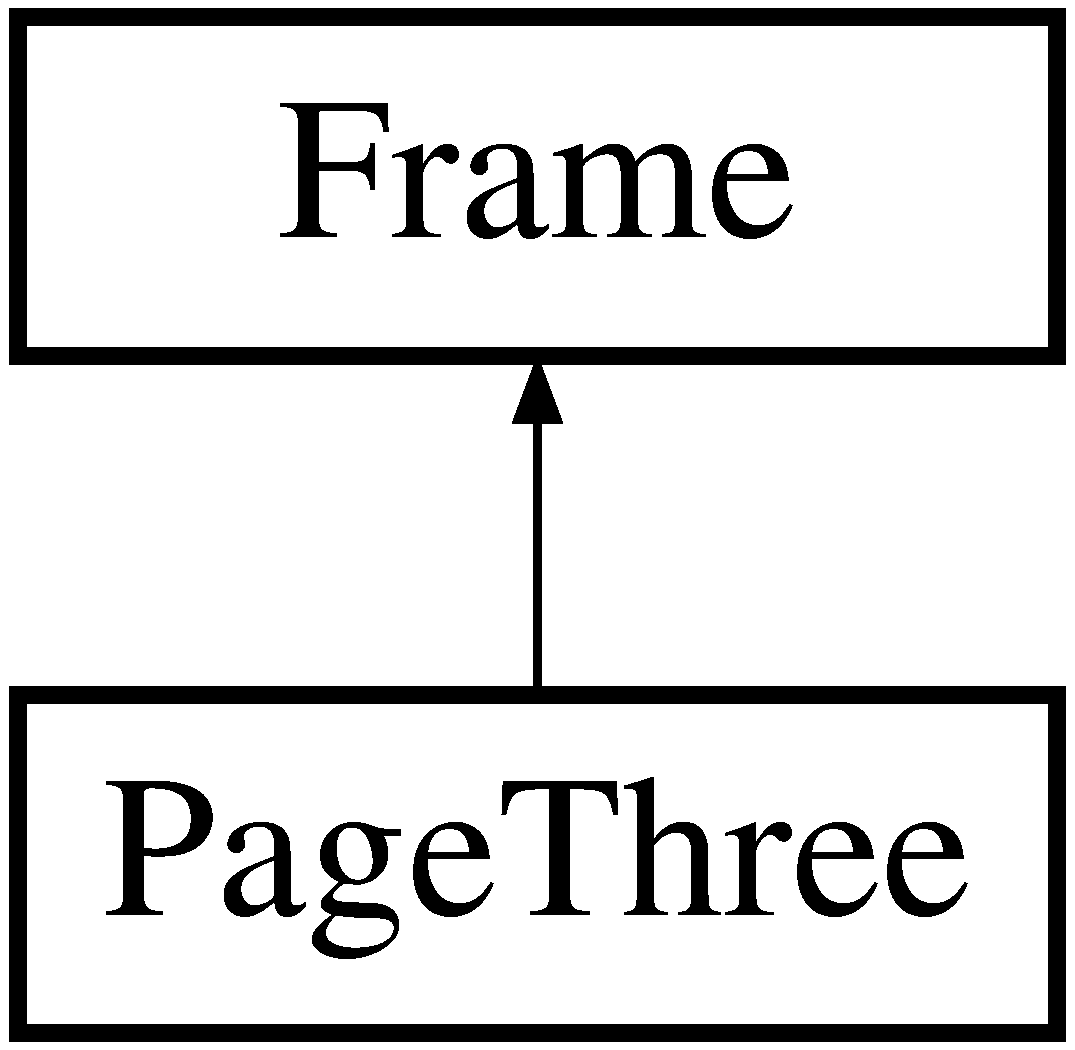
\includegraphics[height=2.000000cm]{class_test_menu_1_1_page_three}
\end{center}
\end{figure}
\subsection*{Public Member Functions}
\begin{DoxyCompactItemize}
\item 
\mbox{\Hypertarget{class_test_menu_1_1_page_three_a558d9afc290e8d1ff922f46114f16631}\label{class_test_menu_1_1_page_three_a558d9afc290e8d1ff922f46114f16631}} 
def {\bfseries \+\_\+\+\_\+init\+\_\+\+\_\+} (self, parent, controller)
\end{DoxyCompactItemize}


The documentation for this class was generated from the following file\+:\begin{DoxyCompactItemize}
\item 
C\+:/\+Users/pestourb/\+Documents/\+Git\+Hub/\+Secure\+Loc/Test\+Menu.\+py\end{DoxyCompactItemize}

\hypertarget{class_test_menu_1_1_page_two}{}\section{Page\+Two Class Reference}
\label{class_test_menu_1_1_page_two}\index{Page\+Two@{Page\+Two}}
Inheritance diagram for Page\+Two\+:\begin{figure}[H]
\begin{center}
\leavevmode
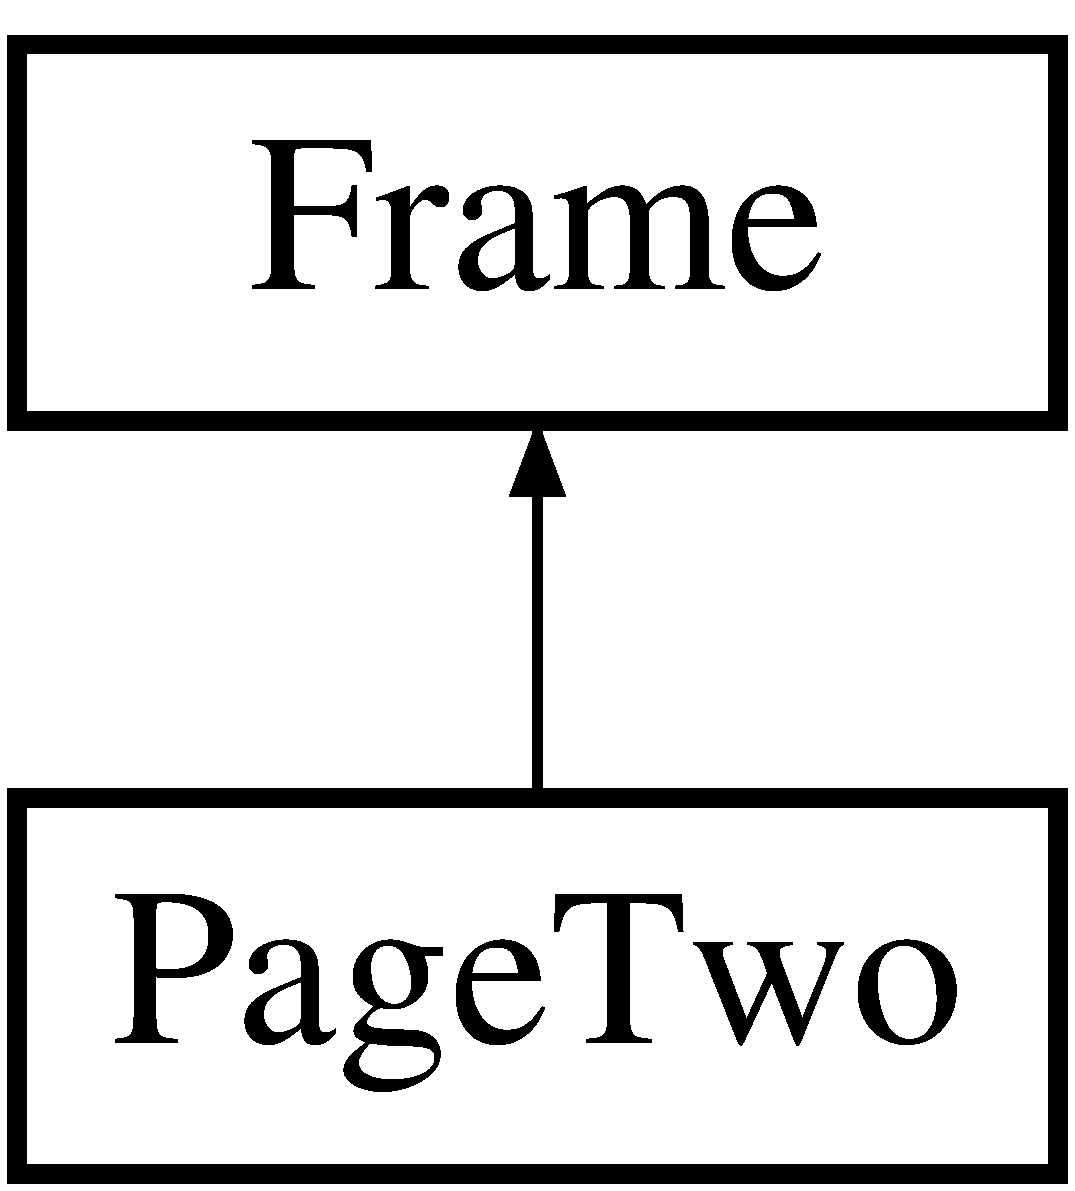
\includegraphics[height=2.000000cm]{class_test_menu_1_1_page_two}
\end{center}
\end{figure}
\subsection*{Public Member Functions}
\begin{DoxyCompactItemize}
\item 
\mbox{\Hypertarget{class_test_menu_1_1_page_two_a558d9afc290e8d1ff922f46114f16631}\label{class_test_menu_1_1_page_two_a558d9afc290e8d1ff922f46114f16631}} 
def {\bfseries \+\_\+\+\_\+init\+\_\+\+\_\+} (self, parent, controller)
\end{DoxyCompactItemize}


The documentation for this class was generated from the following file\+:\begin{DoxyCompactItemize}
\item 
C\+:/\+Users/pestourb/\+Documents/\+Git\+Hub/\+Secure\+Loc/Test\+Menu.\+py\end{DoxyCompactItemize}

\hypertarget{class_emulator_1_1_particle}{}\section{Particle Class Reference}
\label{class_emulator_1_1_particle}\index{Particle@{Particle}}
Inheritance diagram for Particle\+:\begin{figure}[H]
\begin{center}
\leavevmode
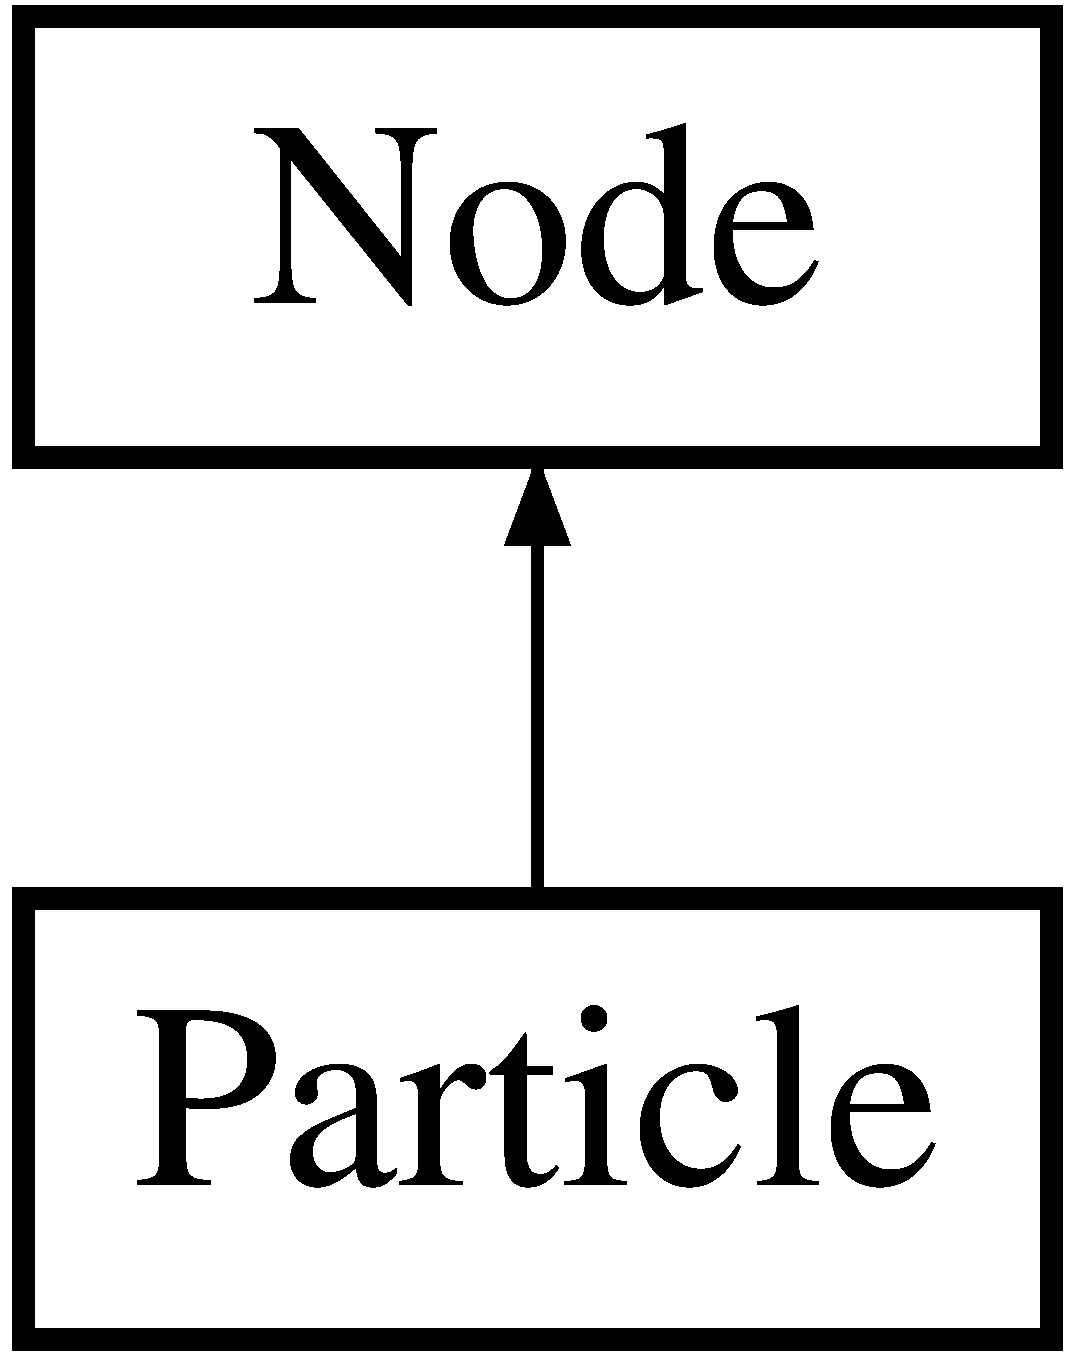
\includegraphics[height=2.000000cm]{class_emulator_1_1_particle}
\end{center}
\end{figure}
\subsection*{Public Member Functions}
\begin{DoxyCompactItemize}
\item 
\mbox{\Hypertarget{class_emulator_1_1_particle_ae6bf6b467ea8b8177ab9fa937a90721c}\label{class_emulator_1_1_particle_ae6bf6b467ea8b8177ab9fa937a90721c}} 
def {\bfseries \+\_\+\+\_\+init\+\_\+\+\_\+} (self, x, y, z)
\item 
\mbox{\Hypertarget{class_emulator_1_1_particle_ab4f4398c3f210fe4ea6e720401357691}\label{class_emulator_1_1_particle_ab4f4398c3f210fe4ea6e720401357691}} 
def {\bfseries show} (self)
\item 
\mbox{\Hypertarget{class_emulator_1_1_particle_ab7a916c513a14fe1dd5ca49be9a9e3a0}\label{class_emulator_1_1_particle_ab7a916c513a14fe1dd5ca49be9a9e3a0}} 
def {\bfseries link\+\_\+previous\+\_\+particle} (self, particle)
\item 
def \mbox{\hyperlink{class_emulator_1_1_particle_a0a2e587249786c6cd49c4c72792667f5}{get\+\_\+depth}} (self)
\item 
def \mbox{\hyperlink{class_emulator_1_1_particle_af84bb961f8e262b28fe9ae6eb4d61e5f}{get\+\_\+speed\+\_\+chain}} (self)
\item 
\mbox{\Hypertarget{class_emulator_1_1_particle_af5b3fcca9b837f7e61d45a1d267d5add}\label{class_emulator_1_1_particle_af5b3fcca9b837f7e61d45a1d267d5add}} 
def {\bfseries get\+\_\+chain\+\_\+likelihood} (self)
\end{DoxyCompactItemize}
\subsection*{Data Fields}
\begin{DoxyCompactItemize}
\item 
\mbox{\Hypertarget{class_emulator_1_1_particle_a0bcacfa65fea4ef51838fdc27cbe79b4}\label{class_emulator_1_1_particle_a0bcacfa65fea4ef51838fdc27cbe79b4}} 
{\bfseries likelihood}
\item 
\mbox{\Hypertarget{class_emulator_1_1_particle_a41e81c4baf16806437e1e2d564570455}\label{class_emulator_1_1_particle_a41e81c4baf16806437e1e2d564570455}} 
{\bfseries previous\+\_\+particle}
\item 
\mbox{\Hypertarget{class_emulator_1_1_particle_ab04a44aead88cfdbd44325ec2cf7a33a}\label{class_emulator_1_1_particle_ab04a44aead88cfdbd44325ec2cf7a33a}} 
{\bfseries speed}
\end{DoxyCompactItemize}


\subsection{Member Function Documentation}
\mbox{\Hypertarget{class_emulator_1_1_particle_a0a2e587249786c6cd49c4c72792667f5}\label{class_emulator_1_1_particle_a0a2e587249786c6cd49c4c72792667f5}} 
\index{Emulator\+::\+Particle@{Emulator\+::\+Particle}!get\+\_\+depth@{get\+\_\+depth}}
\index{get\+\_\+depth@{get\+\_\+depth}!Emulator\+::\+Particle@{Emulator\+::\+Particle}}
\subsubsection{\texorpdfstring{get\+\_\+depth()}{get\_depth()}}
{\footnotesize\ttfamily def get\+\_\+depth (\begin{DoxyParamCaption}\item[{}]{self }\end{DoxyParamCaption})}

\begin{DoxyVerb}Returns the depth of the particle recursive chain\end{DoxyVerb}
 \mbox{\Hypertarget{class_emulator_1_1_particle_af84bb961f8e262b28fe9ae6eb4d61e5f}\label{class_emulator_1_1_particle_af84bb961f8e262b28fe9ae6eb4d61e5f}} 
\index{Emulator\+::\+Particle@{Emulator\+::\+Particle}!get\+\_\+speed\+\_\+chain@{get\+\_\+speed\+\_\+chain}}
\index{get\+\_\+speed\+\_\+chain@{get\+\_\+speed\+\_\+chain}!Emulator\+::\+Particle@{Emulator\+::\+Particle}}
\subsubsection{\texorpdfstring{get\+\_\+speed\+\_\+chain()}{get\_speed\_chain()}}
{\footnotesize\ttfamily def get\+\_\+speed\+\_\+chain (\begin{DoxyParamCaption}\item[{}]{self }\end{DoxyParamCaption})}

\begin{DoxyVerb}returns the vector of the speeds all the particles of the chain \end{DoxyVerb}
 

The documentation for this class was generated from the following file\+:\begin{DoxyCompactItemize}
\item 
C\+:/\+Users/pestourb/\+Documents/\+Git\+Hub/\+Secure\+Loc/Emulator.\+py\end{DoxyCompactItemize}

\hypertarget{classjson_structures_1_1position}{}\section{position Class Reference}
\label{classjson_structures_1_1position}\index{position@{position}}
\subsection*{Public Member Functions}
\begin{DoxyCompactItemize}
\item 
\mbox{\Hypertarget{classjson_structures_1_1position_a90a2418fcab9beabc1adbf51fb20c8a9}\label{classjson_structures_1_1position_a90a2418fcab9beabc1adbf51fb20c8a9}} 
def {\bfseries \+\_\+\+\_\+init\+\_\+\+\_\+} (self, bot\+\_\+id=\textquotesingle{}\textquotesingle{}, x=0, y=0, z=0, mse=None, anchors\+\_\+mse=\{\})
\item 
def \mbox{\hyperlink{classjson_structures_1_1position_a68cc2498d25cf6670863c141957ac262}{export}} (self)
\end{DoxyCompactItemize}
\subsection*{Data Fields}
\begin{DoxyCompactItemize}
\item 
\mbox{\Hypertarget{classjson_structures_1_1position_ac6c8e23f09d95298fc8c3a46143f3dcc}\label{classjson_structures_1_1position_ac6c8e23f09d95298fc8c3a46143f3dcc}} 
{\bfseries bot\+\_\+id}
\item 
\mbox{\Hypertarget{classjson_structures_1_1position_a9336ebf25087d91c818ee6e9ec29f8c1}\label{classjson_structures_1_1position_a9336ebf25087d91c818ee6e9ec29f8c1}} 
{\bfseries x}
\item 
\mbox{\Hypertarget{classjson_structures_1_1position_a2fb1c5cf58867b5bbc9a1b145a86f3a0}\label{classjson_structures_1_1position_a2fb1c5cf58867b5bbc9a1b145a86f3a0}} 
{\bfseries y}
\item 
\mbox{\Hypertarget{classjson_structures_1_1position_a25ed1bcb423b0b7200f485fc5ff71c8e}\label{classjson_structures_1_1position_a25ed1bcb423b0b7200f485fc5ff71c8e}} 
{\bfseries z}
\item 
\mbox{\Hypertarget{classjson_structures_1_1position_ae3588d6b8a60b8198aced11bfe3f2126}\label{classjson_structures_1_1position_ae3588d6b8a60b8198aced11bfe3f2126}} 
{\bfseries mse}
\item 
\mbox{\Hypertarget{classjson_structures_1_1position_ad7205b174179a250431ef104c59f2e73}\label{classjson_structures_1_1position_ad7205b174179a250431ef104c59f2e73}} 
{\bfseries anchors\+\_\+mse}
\end{DoxyCompactItemize}


\subsection{Detailed Description}
\begin{DoxyVerb}Contains the data to log related to positions\end{DoxyVerb}
 

\subsection{Member Function Documentation}
\mbox{\Hypertarget{classjson_structures_1_1position_a68cc2498d25cf6670863c141957ac262}\label{classjson_structures_1_1position_a68cc2498d25cf6670863c141957ac262}} 
\index{json\+Structures\+::position@{json\+Structures\+::position}!export@{export}}
\index{export@{export}!json\+Structures\+::position@{json\+Structures\+::position}}
\subsubsection{\texorpdfstring{export()}{export()}}
{\footnotesize\ttfamily def export (\begin{DoxyParamCaption}\item[{}]{self }\end{DoxyParamCaption})}

\begin{DoxyVerb}returns position as a dictionary\end{DoxyVerb}
 

The documentation for this class was generated from the following file\+:\begin{DoxyCompactItemize}
\item 
C\+:/\+Users/pestourb/\+Documents/\+Git\+Hub/\+Secure\+Loc/json\+Structures.\+py\end{DoxyCompactItemize}

\hypertarget{classranging_1_1_ranging}{}\section{Ranging Class Reference}
\label{classranging_1_1_ranging}\index{Ranging@{Ranging}}
\subsection*{Public Member Functions}
\begin{DoxyCompactItemize}
\item 
\mbox{\Hypertarget{classranging_1_1_ranging_a29a2ca6999cd0cbb296d73f0f1132573}\label{classranging_1_1_ranging_a29a2ca6999cd0cbb296d73f0f1132573}} 
def {\bfseries \+\_\+\+\_\+init\+\_\+\+\_\+} (self, timestamps, lightspeed=L\+I\+G\+H\+T\+S\+P\+E\+ED, timebase=T\+I\+M\+E\+B\+A\+SE)
\item 
\mbox{\Hypertarget{classranging_1_1_ranging_a7d57354a4f9f8d4e428a2539e176493a}\label{classranging_1_1_ranging_a7d57354a4f9f8d4e428a2539e176493a}} 
def {\bfseries T\+WR} (self)
\item 
\mbox{\Hypertarget{classranging_1_1_ranging_a8f189dac28c87f6cff91c4d58b76fbe2}\label{classranging_1_1_ranging_a8f189dac28c87f6cff91c4d58b76fbe2}} 
def {\bfseries get\+Distance} (self, protocol=\textquotesingle{}T\+WR\textquotesingle{})
\end{DoxyCompactItemize}
\subsection*{Data Fields}
\begin{DoxyCompactItemize}
\item 
\mbox{\Hypertarget{classranging_1_1_ranging_ada03328a9187736162c7277d89ef159e}\label{classranging_1_1_ranging_ada03328a9187736162c7277d89ef159e}} 
{\bfseries timestamps}
\item 
\mbox{\Hypertarget{classranging_1_1_ranging_a3139244bfb778557108cda2114f91f3f}\label{classranging_1_1_ranging_a3139244bfb778557108cda2114f91f3f}} 
{\bfseries distance}
\item 
\mbox{\Hypertarget{classranging_1_1_ranging_a15cd30083f8aedfcb4d62a56c87e294a}\label{classranging_1_1_ranging_a15cd30083f8aedfcb4d62a56c87e294a}} 
{\bfseries lightspeed}
\item 
\mbox{\Hypertarget{classranging_1_1_ranging_a3037a14116abb6bcdbf6d94ed5461809}\label{classranging_1_1_ranging_a3037a14116abb6bcdbf6d94ed5461809}} 
{\bfseries timebase}
\end{DoxyCompactItemize}


\subsection{Detailed Description}
\begin{DoxyVerb}contains the low-level ranging protocols such as recomputing the ranging output 
with different protocols on the same date\end{DoxyVerb}
 

The documentation for this class was generated from the following file\+:\begin{DoxyCompactItemize}
\item 
C\+:/\+Users/pestourb/\+Documents/\+Git\+Hub/\+Secure\+Loc/ranging.\+py\end{DoxyCompactItemize}

\hypertarget{classread_rangings_1_1_rangings}{}\section{Rangings Class Reference}
\label{classread_rangings_1_1_rangings}\index{Rangings@{Rangings}}
\subsection*{Public Member Functions}
\begin{DoxyCompactItemize}
\item 
\mbox{\Hypertarget{classread_rangings_1_1_rangings_ad5de178e9da2711c5bc270200dc25568}\label{classread_rangings_1_1_rangings_ad5de178e9da2711c5bc270200dc25568}} 
def {\bfseries \+\_\+\+\_\+init\+\_\+\+\_\+} (self, filename)
\item 
def \mbox{\hyperlink{classread_rangings_1_1_rangings_a4bf6b24f95dbd9e6388503f474e0be05}{get\+\_\+metadata}} (self)
\item 
\mbox{\Hypertarget{classread_rangings_1_1_rangings_a2e0bff0a825b8e6ac6f5e387c1c63306}\label{classread_rangings_1_1_rangings_a2e0bff0a825b8e6ac6f5e387c1c63306}} 
def {\bfseries get\+\_\+measured\+\_\+distances} (self)
\item 
\mbox{\Hypertarget{classread_rangings_1_1_rangings_a50bb794ef6124d0dc9cdc85ce94de73c}\label{classread_rangings_1_1_rangings_a50bb794ef6124d0dc9cdc85ce94de73c}} 
def {\bfseries get\+\_\+actual\+\_\+distances} (self)
\item 
def \mbox{\hyperlink{classread_rangings_1_1_rangings_a9cab236ac56c4f2245c8f87035f736ef}{get\+\_\+anchors}} (self)
\item 
def \mbox{\hyperlink{classread_rangings_1_1_rangings_a31dd1b70ec4bf449637fa2500a516f39}{zero\+\_\+truncating}} (self, id)
\item 
def \mbox{\hyperlink{classread_rangings_1_1_rangings_a3720c2eca68a86eb32876fad24d37b65}{ranging\+\_\+from\+\_\+rp}} (self, rp, anchor\+\_\+name)
\item 
def \mbox{\hyperlink{classread_rangings_1_1_rangings_a993884eadd2abd392aa1b4d0aca03d57}{ranging\+\_\+from\+\_\+pos}} (self, pos, anchor\+\_\+name)
\item 
def \mbox{\hyperlink{classread_rangings_1_1_rangings_ae9f85ff6eeb7be193c52d772e6aeacfb}{distance\+\_\+from\+\_\+rp}} (self, rp, pos)
\item 
def \mbox{\hyperlink{classread_rangings_1_1_rangings_aec61a49900a125b0b6f614e94fba7003}{get\+\_\+coord}} (self, x, y, z)
\item 
def \mbox{\hyperlink{classread_rangings_1_1_rangings_aed4577c8cb31856946ba215ba6b235cc}{get\+\_\+mean}} (self, l)
\item 
\mbox{\Hypertarget{classread_rangings_1_1_rangings_a870abf917024d9f1b7c4de52ae343585}\label{classread_rangings_1_1_rangings_a870abf917024d9f1b7c4de52ae343585}} 
def {\bfseries display\+\_\+rangings} (self, anchor)
\end{DoxyCompactItemize}
\subsection*{Data Fields}
\begin{DoxyCompactItemize}
\item 
\mbox{\Hypertarget{classread_rangings_1_1_rangings_a2ff994e16bf9521154de4cf659a3b689}\label{classread_rangings_1_1_rangings_a2ff994e16bf9521154de4cf659a3b689}} 
{\bfseries filename}
\item 
\mbox{\Hypertarget{classread_rangings_1_1_rangings_a37d874d1d45bc2e5bfa013cddacb8e68}\label{classread_rangings_1_1_rangings_a37d874d1d45bc2e5bfa013cddacb8e68}} 
{\bfseries logs}
\item 
\mbox{\Hypertarget{classread_rangings_1_1_rangings_ac74f5fdcc1c338a24cba634a4f16a1b6}\label{classread_rangings_1_1_rangings_ac74f5fdcc1c338a24cba634a4f16a1b6}} 
{\bfseries anchors\+\_\+dic}
\item 
\mbox{\Hypertarget{classread_rangings_1_1_rangings_adab92eab4a26d12a723b31471ffc8241}\label{classread_rangings_1_1_rangings_adab92eab4a26d12a723b31471ffc8241}} 
{\bfseries measured\+\_\+distances}
\item 
\mbox{\Hypertarget{classread_rangings_1_1_rangings_a5b68d6d2c91370ca44cee7699a3cb1fd}\label{classread_rangings_1_1_rangings_a5b68d6d2c91370ca44cee7699a3cb1fd}} 
{\bfseries anchors\+\_\+pos}
\item 
\mbox{\Hypertarget{classread_rangings_1_1_rangings_a64b8b36116751d566275b722e40bb3a7}\label{classread_rangings_1_1_rangings_a64b8b36116751d566275b722e40bb3a7}} 
{\bfseries comments}
\item 
\mbox{\Hypertarget{classread_rangings_1_1_rangings_a011ffe4ae9802b535701e516a805de4d}\label{classread_rangings_1_1_rangings_a011ffe4ae9802b535701e516a805de4d}} 
{\bfseries actual\+\_\+distances}
\end{DoxyCompactItemize}


\subsection{Detailed Description}
\begin{DoxyVerb}Postprocessing of the ranging data in json files\end{DoxyVerb}
 

\subsection{Member Function Documentation}
\mbox{\Hypertarget{classread_rangings_1_1_rangings_ae9f85ff6eeb7be193c52d772e6aeacfb}\label{classread_rangings_1_1_rangings_ae9f85ff6eeb7be193c52d772e6aeacfb}} 
\index{read\+Rangings\+::\+Rangings@{read\+Rangings\+::\+Rangings}!distance\+\_\+from\+\_\+rp@{distance\+\_\+from\+\_\+rp}}
\index{distance\+\_\+from\+\_\+rp@{distance\+\_\+from\+\_\+rp}!read\+Rangings\+::\+Rangings@{read\+Rangings\+::\+Rangings}}
\subsubsection{\texorpdfstring{distance\+\_\+from\+\_\+rp()}{distance\_from\_rp()}}
{\footnotesize\ttfamily def distance\+\_\+from\+\_\+rp (\begin{DoxyParamCaption}\item[{}]{self,  }\item[{}]{rp,  }\item[{}]{pos }\end{DoxyParamCaption})}

\begin{DoxyVerb}returns the distance between the given position & the given rp\end{DoxyVerb}
 \mbox{\Hypertarget{classread_rangings_1_1_rangings_a9cab236ac56c4f2245c8f87035f736ef}\label{classread_rangings_1_1_rangings_a9cab236ac56c4f2245c8f87035f736ef}} 
\index{read\+Rangings\+::\+Rangings@{read\+Rangings\+::\+Rangings}!get\+\_\+anchors@{get\+\_\+anchors}}
\index{get\+\_\+anchors@{get\+\_\+anchors}!read\+Rangings\+::\+Rangings@{read\+Rangings\+::\+Rangings}}
\subsubsection{\texorpdfstring{get\+\_\+anchors()}{get\_anchors()}}
{\footnotesize\ttfamily def get\+\_\+anchors (\begin{DoxyParamCaption}\item[{}]{self }\end{DoxyParamCaption})}

\begin{DoxyVerb}gets the anchors names & positions from metadata\end{DoxyVerb}
 \mbox{\Hypertarget{classread_rangings_1_1_rangings_aec61a49900a125b0b6f614e94fba7003}\label{classread_rangings_1_1_rangings_aec61a49900a125b0b6f614e94fba7003}} 
\index{read\+Rangings\+::\+Rangings@{read\+Rangings\+::\+Rangings}!get\+\_\+coord@{get\+\_\+coord}}
\index{get\+\_\+coord@{get\+\_\+coord}!read\+Rangings\+::\+Rangings@{read\+Rangings\+::\+Rangings}}
\subsubsection{\texorpdfstring{get\+\_\+coord()}{get\_coord()}}
{\footnotesize\ttfamily def get\+\_\+coord (\begin{DoxyParamCaption}\item[{}]{self,  }\item[{}]{x,  }\item[{}]{y,  }\item[{}]{z }\end{DoxyParamCaption})}

\begin{DoxyVerb}returns the coordinates associated to the given pos on a tiled surface\end{DoxyVerb}
 \mbox{\Hypertarget{classread_rangings_1_1_rangings_aed4577c8cb31856946ba215ba6b235cc}\label{classread_rangings_1_1_rangings_aed4577c8cb31856946ba215ba6b235cc}} 
\index{read\+Rangings\+::\+Rangings@{read\+Rangings\+::\+Rangings}!get\+\_\+mean@{get\+\_\+mean}}
\index{get\+\_\+mean@{get\+\_\+mean}!read\+Rangings\+::\+Rangings@{read\+Rangings\+::\+Rangings}}
\subsubsection{\texorpdfstring{get\+\_\+mean()}{get\_mean()}}
{\footnotesize\ttfamily def get\+\_\+mean (\begin{DoxyParamCaption}\item[{}]{self,  }\item[{}]{l }\end{DoxyParamCaption})}

\begin{DoxyVerb}returns the mean of a list\end{DoxyVerb}
 \mbox{\Hypertarget{classread_rangings_1_1_rangings_a4bf6b24f95dbd9e6388503f474e0be05}\label{classread_rangings_1_1_rangings_a4bf6b24f95dbd9e6388503f474e0be05}} 
\index{read\+Rangings\+::\+Rangings@{read\+Rangings\+::\+Rangings}!get\+\_\+metadata@{get\+\_\+metadata}}
\index{get\+\_\+metadata@{get\+\_\+metadata}!read\+Rangings\+::\+Rangings@{read\+Rangings\+::\+Rangings}}
\subsubsection{\texorpdfstring{get\+\_\+metadata()}{get\_metadata()}}
{\footnotesize\ttfamily def get\+\_\+metadata (\begin{DoxyParamCaption}\item[{}]{self }\end{DoxyParamCaption})}

\begin{DoxyVerb}reads and returns as a dic the metadata in the measurements file\end{DoxyVerb}
 \mbox{\Hypertarget{classread_rangings_1_1_rangings_a993884eadd2abd392aa1b4d0aca03d57}\label{classread_rangings_1_1_rangings_a993884eadd2abd392aa1b4d0aca03d57}} 
\index{read\+Rangings\+::\+Rangings@{read\+Rangings\+::\+Rangings}!ranging\+\_\+from\+\_\+pos@{ranging\+\_\+from\+\_\+pos}}
\index{ranging\+\_\+from\+\_\+pos@{ranging\+\_\+from\+\_\+pos}!read\+Rangings\+::\+Rangings@{read\+Rangings\+::\+Rangings}}
\subsubsection{\texorpdfstring{ranging\+\_\+from\+\_\+pos()}{ranging\_from\_pos()}}
{\footnotesize\ttfamily def ranging\+\_\+from\+\_\+pos (\begin{DoxyParamCaption}\item[{}]{self,  }\item[{}]{pos,  }\item[{}]{anchor\+\_\+name }\end{DoxyParamCaption})}

\begin{DoxyVerb}returns the distance between the given position and the given anchor\end{DoxyVerb}
 \mbox{\Hypertarget{classread_rangings_1_1_rangings_a3720c2eca68a86eb32876fad24d37b65}\label{classread_rangings_1_1_rangings_a3720c2eca68a86eb32876fad24d37b65}} 
\index{read\+Rangings\+::\+Rangings@{read\+Rangings\+::\+Rangings}!ranging\+\_\+from\+\_\+rp@{ranging\+\_\+from\+\_\+rp}}
\index{ranging\+\_\+from\+\_\+rp@{ranging\+\_\+from\+\_\+rp}!read\+Rangings\+::\+Rangings@{read\+Rangings\+::\+Rangings}}
\subsubsection{\texorpdfstring{ranging\+\_\+from\+\_\+rp()}{ranging\_from\_rp()}}
{\footnotesize\ttfamily def ranging\+\_\+from\+\_\+rp (\begin{DoxyParamCaption}\item[{}]{self,  }\item[{}]{rp,  }\item[{}]{anchor\+\_\+name }\end{DoxyParamCaption})}

\begin{DoxyVerb}returns the distance between the given anchor and the given rp\end{DoxyVerb}
 \mbox{\Hypertarget{classread_rangings_1_1_rangings_a31dd1b70ec4bf449637fa2500a516f39}\label{classread_rangings_1_1_rangings_a31dd1b70ec4bf449637fa2500a516f39}} 
\index{read\+Rangings\+::\+Rangings@{read\+Rangings\+::\+Rangings}!zero\+\_\+truncating@{zero\+\_\+truncating}}
\index{zero\+\_\+truncating@{zero\+\_\+truncating}!read\+Rangings\+::\+Rangings@{read\+Rangings\+::\+Rangings}}
\subsubsection{\texorpdfstring{zero\+\_\+truncating()}{zero\_truncating()}}
{\footnotesize\ttfamily def zero\+\_\+truncating (\begin{DoxyParamCaption}\item[{}]{self,  }\item[{}]{id }\end{DoxyParamCaption})}

\begin{DoxyVerb}removes '0' before the id if any\end{DoxyVerb}
 

The documentation for this class was generated from the following file\+:\begin{DoxyCompactItemize}
\item 
C\+:/\+Users/pestourb/\+Documents/\+Git\+Hub/\+Secure\+Loc/read\+Rangings.\+py\end{DoxyCompactItemize}

\hypertarget{class_rendering_1_1_rendered_node}{}\section{Rendered\+Node Class Reference}
\label{class_rendering_1_1_rendered_node}\index{Rendered\+Node@{Rendered\+Node}}
Inheritance diagram for Rendered\+Node\+:\begin{figure}[H]
\begin{center}
\leavevmode
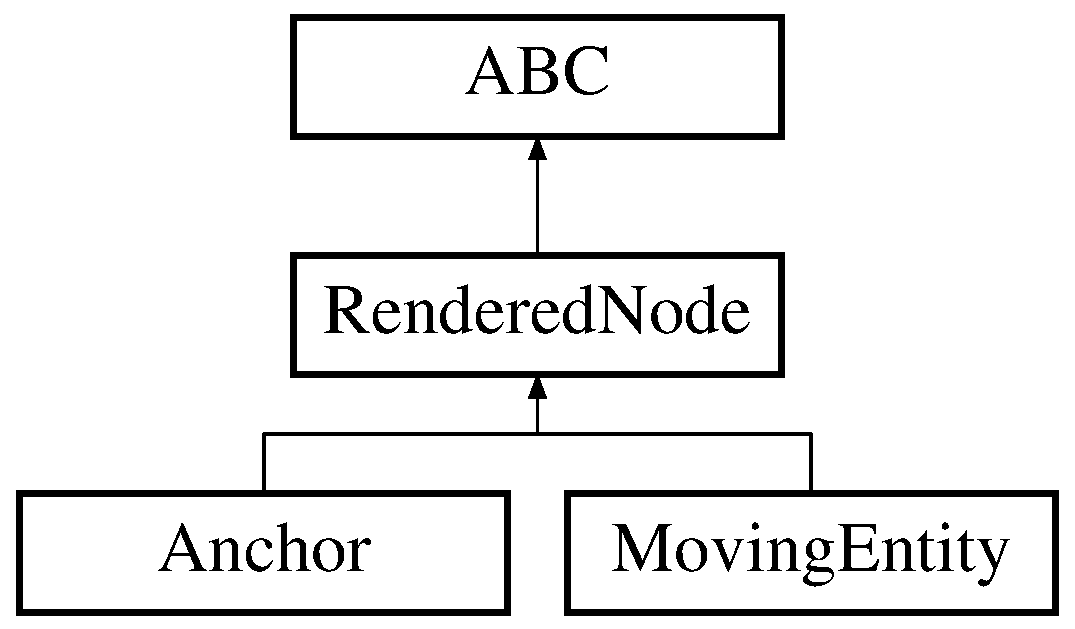
\includegraphics[height=3.000000cm]{class_rendering_1_1_rendered_node}
\end{center}
\end{figure}
\subsection*{Public Member Functions}
\begin{DoxyCompactItemize}
\item 
\mbox{\Hypertarget{class_rendering_1_1_rendered_node_a45e503d244ac0bf916c69c5016664214}\label{class_rendering_1_1_rendered_node_a45e503d244ac0bf916c69c5016664214}} 
def {\bfseries color} (self)
\item 
def \mbox{\hyperlink{class_rendering_1_1_rendered_node_ae531ba5fc89ce010cfdb86441b15eaaa}{shown}} (self)
\item 
def \mbox{\hyperlink{class_rendering_1_1_rendered_node_a73f467422e901c2f8388cedde8228028}{text}} (self)
\item 
def \mbox{\hyperlink{class_rendering_1_1_rendered_node_ad6085aa230d9fd00409dd650b0b549bc}{is\+\_\+\+Anchor}} (self)
\item 
\mbox{\Hypertarget{class_rendering_1_1_rendered_node_a89c968c83617e2fca6e64e74c6478b58}\label{class_rendering_1_1_rendered_node_a89c968c83617e2fca6e64e74c6478b58}} 
def {\bfseries get\+\_\+coordinates} (self)
\item 
\mbox{\Hypertarget{class_rendering_1_1_rendered_node_afc59fd77ac0d0375226e77947f7f6624}\label{class_rendering_1_1_rendered_node_afc59fd77ac0d0375226e77947f7f6624}} 
def {\bfseries set\+\_\+coordinates} (self, x, y, z)
\item 
def \mbox{\hyperlink{class_rendering_1_1_rendered_node_a09f3f97175c16ea6025da871f653d416}{get\+\_\+\+ID}} (self)
\item 
def \mbox{\hyperlink{class_rendering_1_1_rendered_node_a8497086c897585b6ee2234e8728e69e5}{get\+\_\+all\+\_\+distances}} (self)
\item 
def \mbox{\hyperlink{class_rendering_1_1_rendered_node_a48d6e28dbdac1e5f35453b5dfc4eced3}{change\+\_\+color}} (self, color=\textquotesingle{}red\textquotesingle{})
\item 
def \mbox{\hyperlink{class_rendering_1_1_rendered_node_ae5715012ca52873018e51a9c4db43f7c}{displays\+\_\+node\+\_\+at}} (self, x, y, z)
\item 
def \mbox{\hyperlink{class_rendering_1_1_rendered_node_a6feb931cbee18d2d59c63986d969cc22}{move}} (self, pos=None)
\item 
def \mbox{\hyperlink{class_rendering_1_1_rendered_node_a499bd755942d1f9234b6b5aedcc21801}{create\+\_\+sphere}} (self)
\item 
def \mbox{\hyperlink{class_rendering_1_1_rendered_node_ab4f4398c3f210fe4ea6e720401357691}{show}} (self)
\item 
def \mbox{\hyperlink{class_rendering_1_1_rendered_node_ac3c535fd36dc5473ff98017920898352}{hide}} (self)
\item 
def \mbox{\hyperlink{class_rendering_1_1_rendered_node_a882efd96cadb1e70c9583217fa8725f0}{change\+\_\+color}} (self, color)
\item 
def \mbox{\hyperlink{class_rendering_1_1_rendered_node_a6a5edcc7b40b4e6cb4057afc9e6a4025}{get\+\_\+distances\+\_\+as\+\_\+str}} (self)
\item 
def \mbox{\hyperlink{class_rendering_1_1_rendered_node_a2456c7486bc468bd6b0e9277336f6453}{get\+\_\+position\+\_\+as\+\_\+str}} (self)
\item 
def \mbox{\hyperlink{class_rendering_1_1_rendered_node_a0f92537796b85454021dd7ce8e55a3fa}{create\+\_\+text}} (self)
\item 
def \mbox{\hyperlink{class_rendering_1_1_rendered_node_a960251572481fb35d40b7f784de22232}{update\+\_\+text\+\_\+task}} (self, task)
\end{DoxyCompactItemize}
\subsection*{Data Fields}
\begin{DoxyCompactItemize}
\item 
\mbox{\Hypertarget{class_rendering_1_1_rendered_node_a37dbdc30935031c05304482e1be89d8f}\label{class_rendering_1_1_rendered_node_a37dbdc30935031c05304482e1be89d8f}} 
{\bfseries color}
\item 
\mbox{\Hypertarget{class_rendering_1_1_rendered_node_a508cc3106d2c29fe07dc87cbe3ea6927}\label{class_rendering_1_1_rendered_node_a508cc3106d2c29fe07dc87cbe3ea6927}} 
{\bfseries model}
\item 
\mbox{\Hypertarget{class_rendering_1_1_rendered_node_ac6c1eeb684483c821de0ec90f6c47cb9}\label{class_rendering_1_1_rendered_node_ac6c1eeb684483c821de0ec90f6c47cb9}} 
{\bfseries shown}
\item 
\mbox{\Hypertarget{class_rendering_1_1_rendered_node_aa5adb9f4f83816eec03ab763606632a3}\label{class_rendering_1_1_rendered_node_aa5adb9f4f83816eec03ab763606632a3}} 
{\bfseries is\+\_\+\+Anchor}
\item 
\mbox{\Hypertarget{class_rendering_1_1_rendered_node_af575f17e6be3f269b86b041a60560dbf}\label{class_rendering_1_1_rendered_node_af575f17e6be3f269b86b041a60560dbf}} 
{\bfseries text}
\item 
\mbox{\Hypertarget{class_rendering_1_1_rendered_node_a22f45a3cb4f074e609f58ebaeef0ecf9}\label{class_rendering_1_1_rendered_node_a22f45a3cb4f074e609f58ebaeef0ecf9}} 
{\bfseries label}
\item 
\mbox{\Hypertarget{class_rendering_1_1_rendered_node_a9a4324383b31c43c3ba7034d0fb36997}\label{class_rendering_1_1_rendered_node_a9a4324383b31c43c3ba7034d0fb36997}} 
{\bfseries label\+\_\+np}
\end{DoxyCompactItemize}


\subsection{Detailed Description}
\begin{DoxyVerb}Representation of a node in the 3D engine. Anchors & mobile tags are both considered as nodes.
Contains all graphical methods common to all types of nodes\end{DoxyVerb}
 

\subsection{Member Function Documentation}
\mbox{\Hypertarget{class_rendering_1_1_rendered_node_a48d6e28dbdac1e5f35453b5dfc4eced3}\label{class_rendering_1_1_rendered_node_a48d6e28dbdac1e5f35453b5dfc4eced3}} 
\index{Rendering\+::\+Rendered\+Node@{Rendering\+::\+Rendered\+Node}!change\+\_\+color@{change\+\_\+color}}
\index{change\+\_\+color@{change\+\_\+color}!Rendering\+::\+Rendered\+Node@{Rendering\+::\+Rendered\+Node}}
\subsubsection{\texorpdfstring{change\+\_\+color()}{change\_color()}\hspace{0.1cm}{\footnotesize\ttfamily [1/2]}}
{\footnotesize\ttfamily def change\+\_\+color (\begin{DoxyParamCaption}\item[{}]{self,  }\item[{}]{color = {\ttfamily \textquotesingle{}red\textquotesingle{}} }\end{DoxyParamCaption})}

\begin{DoxyVerb}Changes the node color in the 3D engine. Default color is red\end{DoxyVerb}
 \mbox{\Hypertarget{class_rendering_1_1_rendered_node_a882efd96cadb1e70c9583217fa8725f0}\label{class_rendering_1_1_rendered_node_a882efd96cadb1e70c9583217fa8725f0}} 
\index{Rendering\+::\+Rendered\+Node@{Rendering\+::\+Rendered\+Node}!change\+\_\+color@{change\+\_\+color}}
\index{change\+\_\+color@{change\+\_\+color}!Rendering\+::\+Rendered\+Node@{Rendering\+::\+Rendered\+Node}}
\subsubsection{\texorpdfstring{change\+\_\+color()}{change\_color()}\hspace{0.1cm}{\footnotesize\ttfamily [2/2]}}
{\footnotesize\ttfamily def change\+\_\+color (\begin{DoxyParamCaption}\item[{}]{self,  }\item[{}]{color }\end{DoxyParamCaption})}

\begin{DoxyVerb}chanegs the color of the node rendition in the 3D engine\end{DoxyVerb}
 \mbox{\Hypertarget{class_rendering_1_1_rendered_node_a499bd755942d1f9234b6b5aedcc21801}\label{class_rendering_1_1_rendered_node_a499bd755942d1f9234b6b5aedcc21801}} 
\index{Rendering\+::\+Rendered\+Node@{Rendering\+::\+Rendered\+Node}!create\+\_\+sphere@{create\+\_\+sphere}}
\index{create\+\_\+sphere@{create\+\_\+sphere}!Rendering\+::\+Rendered\+Node@{Rendering\+::\+Rendered\+Node}}
\subsubsection{\texorpdfstring{create\+\_\+sphere()}{create\_sphere()}}
{\footnotesize\ttfamily def create\+\_\+sphere (\begin{DoxyParamCaption}\item[{}]{self }\end{DoxyParamCaption})}

\begin{DoxyVerb}Create the node representation for the 3D world\end{DoxyVerb}
 \mbox{\Hypertarget{class_rendering_1_1_rendered_node_a0f92537796b85454021dd7ce8e55a3fa}\label{class_rendering_1_1_rendered_node_a0f92537796b85454021dd7ce8e55a3fa}} 
\index{Rendering\+::\+Rendered\+Node@{Rendering\+::\+Rendered\+Node}!create\+\_\+text@{create\+\_\+text}}
\index{create\+\_\+text@{create\+\_\+text}!Rendering\+::\+Rendered\+Node@{Rendering\+::\+Rendered\+Node}}
\subsubsection{\texorpdfstring{create\+\_\+text()}{create\_text()}}
{\footnotesize\ttfamily def create\+\_\+text (\begin{DoxyParamCaption}\item[{}]{self }\end{DoxyParamCaption})}

\begin{DoxyVerb}Displays distance above the node representation.
If multiple distance are given, they all displayed\end{DoxyVerb}
 \mbox{\Hypertarget{class_rendering_1_1_rendered_node_ae5715012ca52873018e51a9c4db43f7c}\label{class_rendering_1_1_rendered_node_ae5715012ca52873018e51a9c4db43f7c}} 
\index{Rendering\+::\+Rendered\+Node@{Rendering\+::\+Rendered\+Node}!displays\+\_\+node\+\_\+at@{displays\+\_\+node\+\_\+at}}
\index{displays\+\_\+node\+\_\+at@{displays\+\_\+node\+\_\+at}!Rendering\+::\+Rendered\+Node@{Rendering\+::\+Rendered\+Node}}
\subsubsection{\texorpdfstring{displays\+\_\+node\+\_\+at()}{displays\_node\_at()}}
{\footnotesize\ttfamily def displays\+\_\+node\+\_\+at (\begin{DoxyParamCaption}\item[{}]{self,  }\item[{}]{x,  }\item[{}]{y,  }\item[{}]{z }\end{DoxyParamCaption})}

\begin{DoxyVerb}Displays the node at the given coordinates.
Note that this only affects the representation of the node in the 3D engine, not the actual coordinates.
Use move instead in the latter case.\end{DoxyVerb}
 \mbox{\Hypertarget{class_rendering_1_1_rendered_node_a8497086c897585b6ee2234e8728e69e5}\label{class_rendering_1_1_rendered_node_a8497086c897585b6ee2234e8728e69e5}} 
\index{Rendering\+::\+Rendered\+Node@{Rendering\+::\+Rendered\+Node}!get\+\_\+all\+\_\+distances@{get\+\_\+all\+\_\+distances}}
\index{get\+\_\+all\+\_\+distances@{get\+\_\+all\+\_\+distances}!Rendering\+::\+Rendered\+Node@{Rendering\+::\+Rendered\+Node}}
\subsubsection{\texorpdfstring{get\+\_\+all\+\_\+distances()}{get\_all\_distances()}}
{\footnotesize\ttfamily def get\+\_\+all\+\_\+distances (\begin{DoxyParamCaption}\item[{}]{self }\end{DoxyParamCaption})}

\begin{DoxyVerb}returns all the distances measured by the node\end{DoxyVerb}
 \mbox{\Hypertarget{class_rendering_1_1_rendered_node_a6a5edcc7b40b4e6cb4057afc9e6a4025}\label{class_rendering_1_1_rendered_node_a6a5edcc7b40b4e6cb4057afc9e6a4025}} 
\index{Rendering\+::\+Rendered\+Node@{Rendering\+::\+Rendered\+Node}!get\+\_\+distances\+\_\+as\+\_\+str@{get\+\_\+distances\+\_\+as\+\_\+str}}
\index{get\+\_\+distances\+\_\+as\+\_\+str@{get\+\_\+distances\+\_\+as\+\_\+str}!Rendering\+::\+Rendered\+Node@{Rendering\+::\+Rendered\+Node}}
\subsubsection{\texorpdfstring{get\+\_\+distances\+\_\+as\+\_\+str()}{get\_distances\_as\_str()}}
{\footnotesize\ttfamily def get\+\_\+distances\+\_\+as\+\_\+str (\begin{DoxyParamCaption}\item[{}]{self }\end{DoxyParamCaption})}

\begin{DoxyVerb}converts the distances measured by the node into a string.
The string is formatted as 'distance1 / distance2/... distance n'
The order given follows the order of IDs\end{DoxyVerb}
 \mbox{\Hypertarget{class_rendering_1_1_rendered_node_a09f3f97175c16ea6025da871f653d416}\label{class_rendering_1_1_rendered_node_a09f3f97175c16ea6025da871f653d416}} 
\index{Rendering\+::\+Rendered\+Node@{Rendering\+::\+Rendered\+Node}!get\+\_\+\+ID@{get\+\_\+\+ID}}
\index{get\+\_\+\+ID@{get\+\_\+\+ID}!Rendering\+::\+Rendered\+Node@{Rendering\+::\+Rendered\+Node}}
\subsubsection{\texorpdfstring{get\+\_\+\+I\+D()}{get\_ID()}}
{\footnotesize\ttfamily def get\+\_\+\+ID (\begin{DoxyParamCaption}\item[{}]{self }\end{DoxyParamCaption})}

\begin{DoxyVerb}returns node ID; can be used to find out if the node is an anchor or a tag\end{DoxyVerb}
 \mbox{\Hypertarget{class_rendering_1_1_rendered_node_a2456c7486bc468bd6b0e9277336f6453}\label{class_rendering_1_1_rendered_node_a2456c7486bc468bd6b0e9277336f6453}} 
\index{Rendering\+::\+Rendered\+Node@{Rendering\+::\+Rendered\+Node}!get\+\_\+position\+\_\+as\+\_\+str@{get\+\_\+position\+\_\+as\+\_\+str}}
\index{get\+\_\+position\+\_\+as\+\_\+str@{get\+\_\+position\+\_\+as\+\_\+str}!Rendering\+::\+Rendered\+Node@{Rendering\+::\+Rendered\+Node}}
\subsubsection{\texorpdfstring{get\+\_\+position\+\_\+as\+\_\+str()}{get\_position\_as\_str()}}
{\footnotesize\ttfamily def get\+\_\+position\+\_\+as\+\_\+str (\begin{DoxyParamCaption}\item[{}]{self }\end{DoxyParamCaption})}

\begin{DoxyVerb}converts the node position into a string\end{DoxyVerb}
 \mbox{\Hypertarget{class_rendering_1_1_rendered_node_ac3c535fd36dc5473ff98017920898352}\label{class_rendering_1_1_rendered_node_ac3c535fd36dc5473ff98017920898352}} 
\index{Rendering\+::\+Rendered\+Node@{Rendering\+::\+Rendered\+Node}!hide@{hide}}
\index{hide@{hide}!Rendering\+::\+Rendered\+Node@{Rendering\+::\+Rendered\+Node}}
\subsubsection{\texorpdfstring{hide()}{hide()}}
{\footnotesize\ttfamily def hide (\begin{DoxyParamCaption}\item[{}]{self }\end{DoxyParamCaption})}

\begin{DoxyVerb}Hides node in the 3D engine\end{DoxyVerb}
 \mbox{\Hypertarget{class_rendering_1_1_rendered_node_ad6085aa230d9fd00409dd650b0b549bc}\label{class_rendering_1_1_rendered_node_ad6085aa230d9fd00409dd650b0b549bc}} 
\index{Rendering\+::\+Rendered\+Node@{Rendering\+::\+Rendered\+Node}!is\+\_\+\+Anchor@{is\+\_\+\+Anchor}}
\index{is\+\_\+\+Anchor@{is\+\_\+\+Anchor}!Rendering\+::\+Rendered\+Node@{Rendering\+::\+Rendered\+Node}}
\subsubsection{\texorpdfstring{is\+\_\+\+Anchor()}{is\_Anchor()}}
{\footnotesize\ttfamily def is\+\_\+\+Anchor (\begin{DoxyParamCaption}\item[{}]{self }\end{DoxyParamCaption})}

\begin{DoxyVerb}whether the node is an anchor or not\end{DoxyVerb}
 \mbox{\Hypertarget{class_rendering_1_1_rendered_node_a6feb931cbee18d2d59c63986d969cc22}\label{class_rendering_1_1_rendered_node_a6feb931cbee18d2d59c63986d969cc22}} 
\index{Rendering\+::\+Rendered\+Node@{Rendering\+::\+Rendered\+Node}!move@{move}}
\index{move@{move}!Rendering\+::\+Rendered\+Node@{Rendering\+::\+Rendered\+Node}}
\subsubsection{\texorpdfstring{move()}{move()}}
{\footnotesize\ttfamily def move (\begin{DoxyParamCaption}\item[{}]{self,  }\item[{}]{pos = {\ttfamily None} }\end{DoxyParamCaption})}

\begin{DoxyVerb}Moves the node at the given position.
This affects both the position of the node in the 3D engine and the sotred coordinates
Calling without argument will move to the current position.
Giving position as tuple in input will define this position as the current position\end{DoxyVerb}
 \mbox{\Hypertarget{class_rendering_1_1_rendered_node_ab4f4398c3f210fe4ea6e720401357691}\label{class_rendering_1_1_rendered_node_ab4f4398c3f210fe4ea6e720401357691}} 
\index{Rendering\+::\+Rendered\+Node@{Rendering\+::\+Rendered\+Node}!show@{show}}
\index{show@{show}!Rendering\+::\+Rendered\+Node@{Rendering\+::\+Rendered\+Node}}
\subsubsection{\texorpdfstring{show()}{show()}}
{\footnotesize\ttfamily def show (\begin{DoxyParamCaption}\item[{}]{self }\end{DoxyParamCaption})}

\begin{DoxyVerb}Displays node in the 3D engine\end{DoxyVerb}
 \mbox{\Hypertarget{class_rendering_1_1_rendered_node_ae531ba5fc89ce010cfdb86441b15eaaa}\label{class_rendering_1_1_rendered_node_ae531ba5fc89ce010cfdb86441b15eaaa}} 
\index{Rendering\+::\+Rendered\+Node@{Rendering\+::\+Rendered\+Node}!shown@{shown}}
\index{shown@{shown}!Rendering\+::\+Rendered\+Node@{Rendering\+::\+Rendered\+Node}}
\subsubsection{\texorpdfstring{shown()}{shown()}}
{\footnotesize\ttfamily def shown (\begin{DoxyParamCaption}\item[{}]{self }\end{DoxyParamCaption})}

\begin{DoxyVerb}whether the node is visible or not\end{DoxyVerb}
 \mbox{\Hypertarget{class_rendering_1_1_rendered_node_a73f467422e901c2f8388cedde8228028}\label{class_rendering_1_1_rendered_node_a73f467422e901c2f8388cedde8228028}} 
\index{Rendering\+::\+Rendered\+Node@{Rendering\+::\+Rendered\+Node}!text@{text}}
\index{text@{text}!Rendering\+::\+Rendered\+Node@{Rendering\+::\+Rendered\+Node}}
\subsubsection{\texorpdfstring{text()}{text()}}
{\footnotesize\ttfamily def text (\begin{DoxyParamCaption}\item[{}]{self }\end{DoxyParamCaption})}

\begin{DoxyVerb}text displayed above the node\end{DoxyVerb}
 \mbox{\Hypertarget{class_rendering_1_1_rendered_node_a960251572481fb35d40b7f784de22232}\label{class_rendering_1_1_rendered_node_a960251572481fb35d40b7f784de22232}} 
\index{Rendering\+::\+Rendered\+Node@{Rendering\+::\+Rendered\+Node}!update\+\_\+text\+\_\+task@{update\+\_\+text\+\_\+task}}
\index{update\+\_\+text\+\_\+task@{update\+\_\+text\+\_\+task}!Rendering\+::\+Rendered\+Node@{Rendering\+::\+Rendered\+Node}}
\subsubsection{\texorpdfstring{update\+\_\+text\+\_\+task()}{update\_text\_task()}}
{\footnotesize\ttfamily def update\+\_\+text\+\_\+task (\begin{DoxyParamCaption}\item[{}]{self,  }\item[{}]{task }\end{DoxyParamCaption})}

\begin{DoxyVerb}Updates the text angle for it to always face the camera\end{DoxyVerb}
 

The documentation for this class was generated from the following file\+:\begin{DoxyCompactItemize}
\item 
C\+:/\+Users/pestourb/\+Documents/\+Git\+Hub/\+Secure\+Loc/Rendering.\+py\end{DoxyCompactItemize}

\hypertarget{class_rendering_stub_1_1_rendered_node}{}\section{Rendered\+Node Class Reference}
\label{class_rendering_stub_1_1_rendered_node}\index{Rendered\+Node@{Rendered\+Node}}
Inheritance diagram for Rendered\+Node\+:\begin{figure}[H]
\begin{center}
\leavevmode
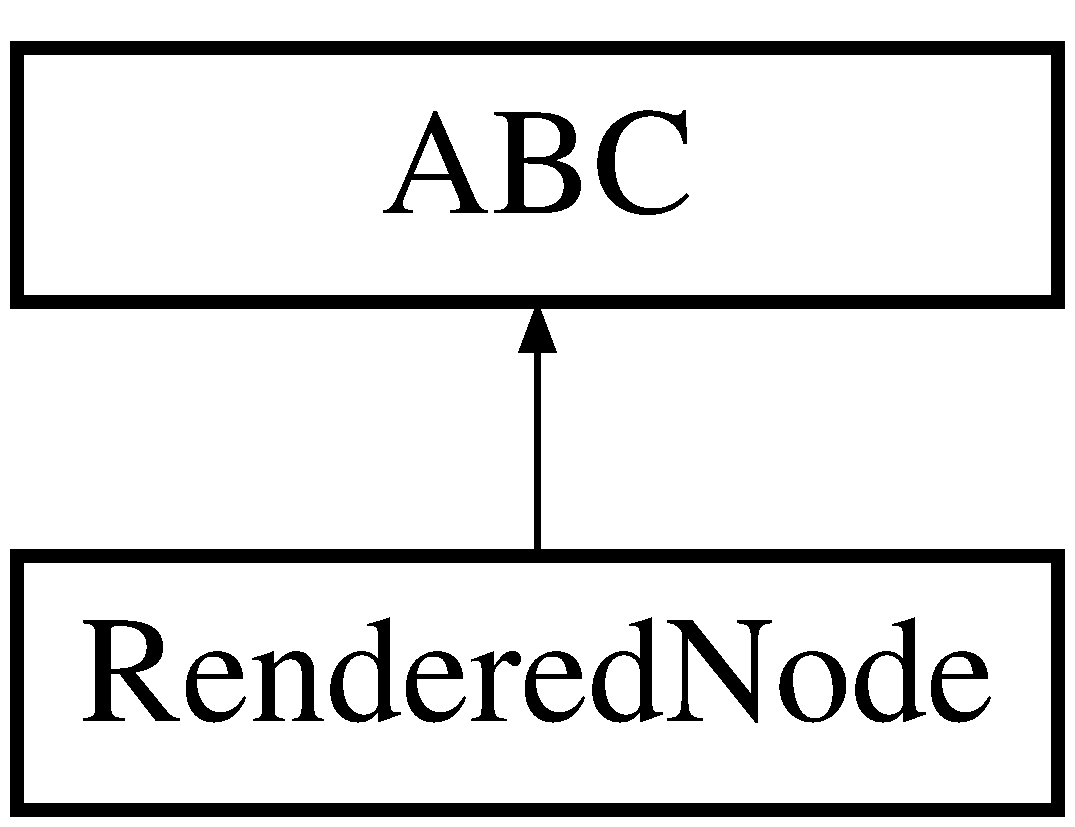
\includegraphics[height=2.000000cm]{class_rendering_stub_1_1_rendered_node}
\end{center}
\end{figure}
\subsection*{Public Member Functions}
\begin{DoxyCompactItemize}
\item 
\mbox{\Hypertarget{class_rendering_stub_1_1_rendered_node_a45e503d244ac0bf916c69c5016664214}\label{class_rendering_stub_1_1_rendered_node_a45e503d244ac0bf916c69c5016664214}} 
def {\bfseries color} (self)
\item 
\mbox{\Hypertarget{class_rendering_stub_1_1_rendered_node_ae531ba5fc89ce010cfdb86441b15eaaa}\label{class_rendering_stub_1_1_rendered_node_ae531ba5fc89ce010cfdb86441b15eaaa}} 
def {\bfseries shown} (self)
\item 
\mbox{\Hypertarget{class_rendering_stub_1_1_rendered_node_a73f467422e901c2f8388cedde8228028}\label{class_rendering_stub_1_1_rendered_node_a73f467422e901c2f8388cedde8228028}} 
def {\bfseries text} (self)
\item 
\mbox{\Hypertarget{class_rendering_stub_1_1_rendered_node_ad6085aa230d9fd00409dd650b0b549bc}\label{class_rendering_stub_1_1_rendered_node_ad6085aa230d9fd00409dd650b0b549bc}} 
def {\bfseries is\+\_\+\+Anchor} (self)
\item 
\mbox{\Hypertarget{class_rendering_stub_1_1_rendered_node_a89c968c83617e2fca6e64e74c6478b58}\label{class_rendering_stub_1_1_rendered_node_a89c968c83617e2fca6e64e74c6478b58}} 
def {\bfseries get\+\_\+coordinates} (self)
\item 
\mbox{\Hypertarget{class_rendering_stub_1_1_rendered_node_afc59fd77ac0d0375226e77947f7f6624}\label{class_rendering_stub_1_1_rendered_node_afc59fd77ac0d0375226e77947f7f6624}} 
def {\bfseries set\+\_\+coordinates} (self, x, y, z)
\item 
\mbox{\Hypertarget{class_rendering_stub_1_1_rendered_node_a09f3f97175c16ea6025da871f653d416}\label{class_rendering_stub_1_1_rendered_node_a09f3f97175c16ea6025da871f653d416}} 
def {\bfseries get\+\_\+\+ID} (self)
\item 
\mbox{\Hypertarget{class_rendering_stub_1_1_rendered_node_a8497086c897585b6ee2234e8728e69e5}\label{class_rendering_stub_1_1_rendered_node_a8497086c897585b6ee2234e8728e69e5}} 
def {\bfseries get\+\_\+all\+\_\+distances} (self)
\item 
\mbox{\Hypertarget{class_rendering_stub_1_1_rendered_node_a48d6e28dbdac1e5f35453b5dfc4eced3}\label{class_rendering_stub_1_1_rendered_node_a48d6e28dbdac1e5f35453b5dfc4eced3}} 
def {\bfseries change\+\_\+color} (self, color=\textquotesingle{}red\textquotesingle{})
\item 
\mbox{\Hypertarget{class_rendering_stub_1_1_rendered_node_ae5715012ca52873018e51a9c4db43f7c}\label{class_rendering_stub_1_1_rendered_node_ae5715012ca52873018e51a9c4db43f7c}} 
def {\bfseries displays\+\_\+node\+\_\+at} (self, x, y, z)
\item 
\mbox{\Hypertarget{class_rendering_stub_1_1_rendered_node_a6feb931cbee18d2d59c63986d969cc22}\label{class_rendering_stub_1_1_rendered_node_a6feb931cbee18d2d59c63986d969cc22}} 
def {\bfseries move} (self, pos=None)
\item 
\mbox{\Hypertarget{class_rendering_stub_1_1_rendered_node_a499bd755942d1f9234b6b5aedcc21801}\label{class_rendering_stub_1_1_rendered_node_a499bd755942d1f9234b6b5aedcc21801}} 
def {\bfseries create\+\_\+sphere} (self)
\item 
\mbox{\Hypertarget{class_rendering_stub_1_1_rendered_node_ab4f4398c3f210fe4ea6e720401357691}\label{class_rendering_stub_1_1_rendered_node_ab4f4398c3f210fe4ea6e720401357691}} 
def {\bfseries show} (self)
\item 
\mbox{\Hypertarget{class_rendering_stub_1_1_rendered_node_ac3c535fd36dc5473ff98017920898352}\label{class_rendering_stub_1_1_rendered_node_ac3c535fd36dc5473ff98017920898352}} 
def {\bfseries hide} (self)
\item 
\mbox{\Hypertarget{class_rendering_stub_1_1_rendered_node_a6a5edcc7b40b4e6cb4057afc9e6a4025}\label{class_rendering_stub_1_1_rendered_node_a6a5edcc7b40b4e6cb4057afc9e6a4025}} 
def {\bfseries get\+\_\+distances\+\_\+as\+\_\+str} (self)
\item 
\mbox{\Hypertarget{class_rendering_stub_1_1_rendered_node_a2456c7486bc468bd6b0e9277336f6453}\label{class_rendering_stub_1_1_rendered_node_a2456c7486bc468bd6b0e9277336f6453}} 
def {\bfseries get\+\_\+position\+\_\+as\+\_\+str} (self)
\item 
\mbox{\Hypertarget{class_rendering_stub_1_1_rendered_node_a0f92537796b85454021dd7ce8e55a3fa}\label{class_rendering_stub_1_1_rendered_node_a0f92537796b85454021dd7ce8e55a3fa}} 
def {\bfseries create\+\_\+text} (self)
\item 
\mbox{\Hypertarget{class_rendering_stub_1_1_rendered_node_a960251572481fb35d40b7f784de22232}\label{class_rendering_stub_1_1_rendered_node_a960251572481fb35d40b7f784de22232}} 
def {\bfseries update\+\_\+text\+\_\+task} (self, \mbox{\hyperlink{class_rendering_stub_1_1task}{task}})
\end{DoxyCompactItemize}


\subsection{Detailed Description}
\begin{DoxyVerb}Stub for node rendering in the 3D engine.
Will be used automatically if the 3D engines packages are not installed
or if headless mode is being used.\end{DoxyVerb}
 

The documentation for this class was generated from the following file\+:\begin{DoxyCompactItemize}
\item 
C\+:/\+Users/pestourb/\+Documents/\+Git\+Hub/\+Secure\+Loc/Rendering\+Stub.\+py\end{DoxyCompactItemize}

\hypertarget{class_rendering_1_1_rendered_world}{}\section{Rendered\+World Class Reference}
\label{class_rendering_1_1_rendered_world}\index{Rendered\+World@{Rendered\+World}}
Inheritance diagram for Rendered\+World\+:\begin{figure}[H]
\begin{center}
\leavevmode
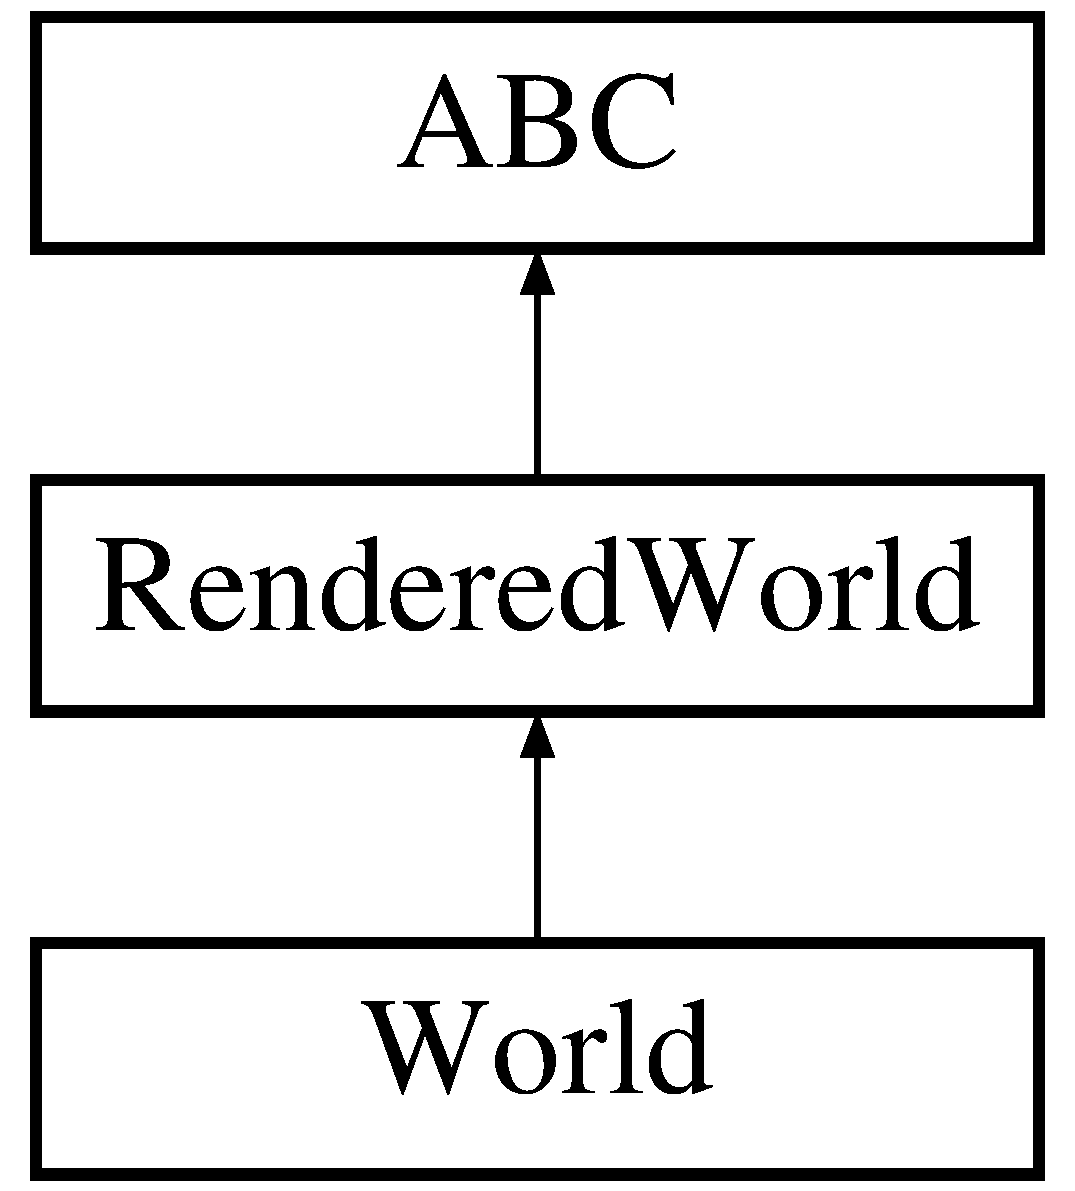
\includegraphics[height=3.000000cm]{class_rendering_1_1_rendered_world}
\end{center}
\end{figure}
\subsection*{Public Member Functions}
\begin{DoxyCompactItemize}
\item 
def \mbox{\hyperlink{class_rendering_1_1_rendered_world_a4c41b83d0d7ca78d6aa31cabe4cf0949}{create\+\_\+grid}} (self)
\end{DoxyCompactItemize}


\subsection{Detailed Description}
\begin{DoxyVerb}Representation of the World in the 3D engine.\end{DoxyVerb}
 

\subsection{Member Function Documentation}
\mbox{\Hypertarget{class_rendering_1_1_rendered_world_a4c41b83d0d7ca78d6aa31cabe4cf0949}\label{class_rendering_1_1_rendered_world_a4c41b83d0d7ca78d6aa31cabe4cf0949}} 
\index{Rendering\+::\+Rendered\+World@{Rendering\+::\+Rendered\+World}!create\+\_\+grid@{create\+\_\+grid}}
\index{create\+\_\+grid@{create\+\_\+grid}!Rendering\+::\+Rendered\+World@{Rendering\+::\+Rendered\+World}}
\subsubsection{\texorpdfstring{create\+\_\+grid()}{create\_grid()}}
{\footnotesize\ttfamily def create\+\_\+grid (\begin{DoxyParamCaption}\item[{}]{self }\end{DoxyParamCaption})}

\begin{DoxyVerb}Create the ground grid\end{DoxyVerb}
 

The documentation for this class was generated from the following file\+:\begin{DoxyCompactItemize}
\item 
C\+:/\+Users/pestourb/\+Documents/\+Git\+Hub/\+Secure\+Loc/Rendering.\+py\end{DoxyCompactItemize}

\hypertarget{class_rendering_stub_1_1_rendered_world}{}\section{Rendered\+World Class Reference}
\label{class_rendering_stub_1_1_rendered_world}\index{Rendered\+World@{Rendered\+World}}
Inheritance diagram for Rendered\+World\+:\begin{figure}[H]
\begin{center}
\leavevmode
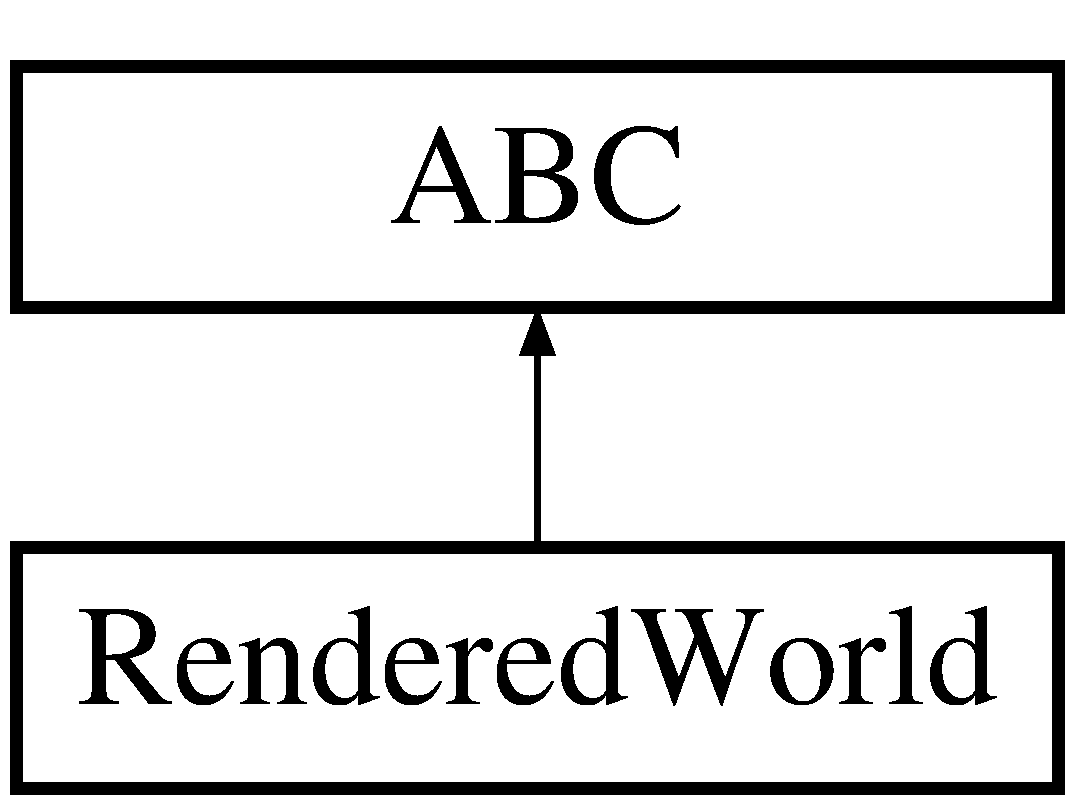
\includegraphics[height=2.000000cm]{class_rendering_stub_1_1_rendered_world}
\end{center}
\end{figure}
\subsection*{Public Member Functions}
\begin{DoxyCompactItemize}
\item 
\mbox{\Hypertarget{class_rendering_stub_1_1_rendered_world_a4c41b83d0d7ca78d6aa31cabe4cf0949}\label{class_rendering_stub_1_1_rendered_world_a4c41b83d0d7ca78d6aa31cabe4cf0949}} 
def {\bfseries create\+\_\+grid} (self)
\end{DoxyCompactItemize}


\subsection{Detailed Description}
\begin{DoxyVerb}Stub for 3D engine World.\end{DoxyVerb}
 

The documentation for this class was generated from the following file\+:\begin{DoxyCompactItemize}
\item 
C\+:/\+Users/pestourb/\+Documents/\+Git\+Hub/\+Secure\+Loc/Rendering\+Stub.\+py\end{DoxyCompactItemize}

\hypertarget{class_rendering_stub_1_1_renderer}{}\section{Renderer Class Reference}
\label{class_rendering_stub_1_1_renderer}\index{Renderer@{Renderer}}
Inheritance diagram for Renderer\+:\begin{figure}[H]
\begin{center}
\leavevmode
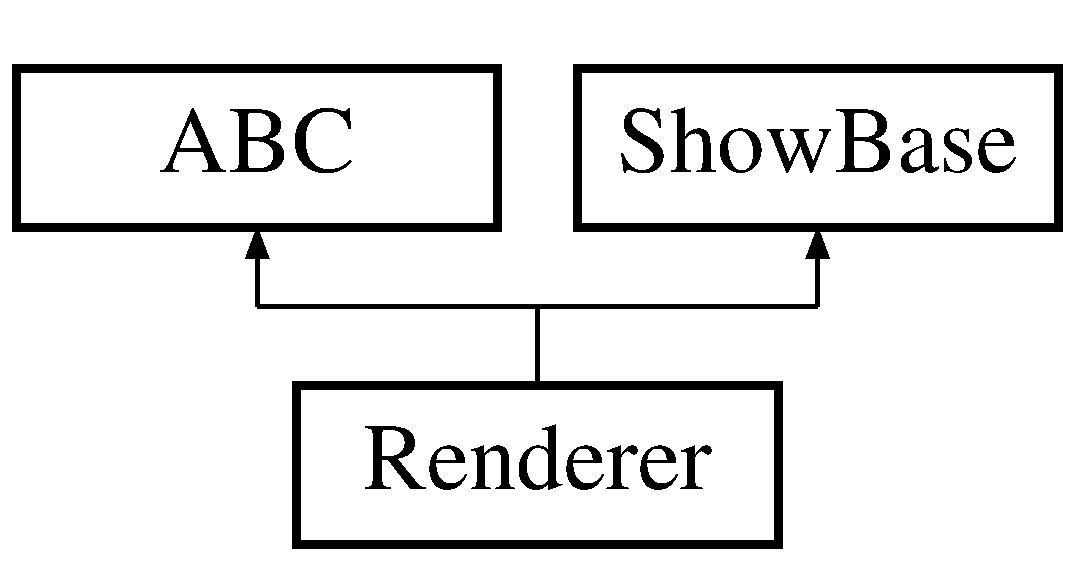
\includegraphics[height=2.000000cm]{class_rendering_stub_1_1_renderer}
\end{center}
\end{figure}
\subsection*{Public Member Functions}
\begin{DoxyCompactItemize}
\item 
\mbox{\Hypertarget{class_rendering_stub_1_1_renderer_af4c0dae777b9590cfc07035425b4d36f}\label{class_rendering_stub_1_1_renderer_af4c0dae777b9590cfc07035425b4d36f}} 
def {\bfseries init\+\_\+render} (self)
\end{DoxyCompactItemize}


\subsection{Detailed Description}
\begin{DoxyVerb}Stub for the interface between the Rendering engine and the main application.
Will be used automatically if the 3D engines packages are not installed
or if headless mode is being used.\end{DoxyVerb}
 

The documentation for this class was generated from the following file\+:\begin{DoxyCompactItemize}
\item 
C\+:/\+Users/pestourb/\+Documents/\+Git\+Hub/\+Secure\+Loc/Rendering\+Stub.\+py\end{DoxyCompactItemize}

\hypertarget{class_rendering_1_1_renderer}{}\section{Renderer Class Reference}
\label{class_rendering_1_1_renderer}\index{Renderer@{Renderer}}
Inheritance diagram for Renderer\+:\begin{figure}[H]
\begin{center}
\leavevmode
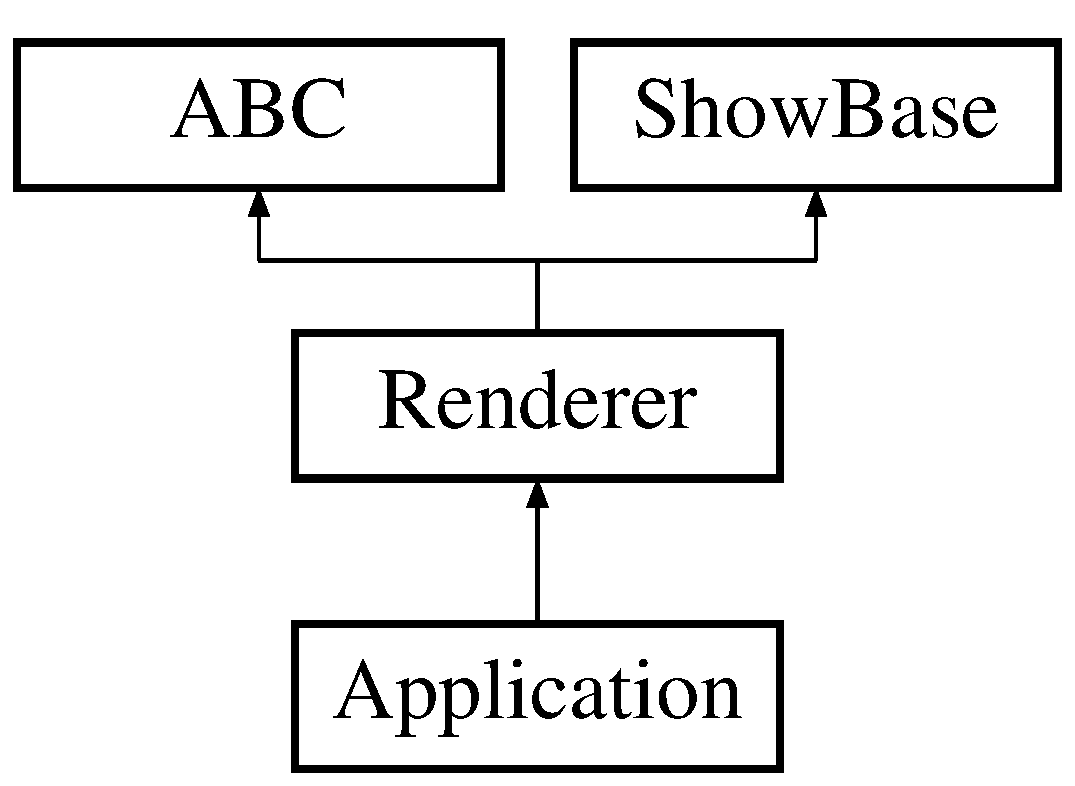
\includegraphics[height=3.000000cm]{class_rendering_1_1_renderer}
\end{center}
\end{figure}
\subsection*{Public Member Functions}
\begin{DoxyCompactItemize}
\item 
def \mbox{\hyperlink{class_rendering_1_1_renderer_af4c0dae777b9590cfc07035425b4d36f}{init\+\_\+render}} (self)
\end{DoxyCompactItemize}
\subsection*{Data Fields}
\begin{DoxyCompactItemize}
\item 
\mbox{\Hypertarget{class_rendering_1_1_renderer_ae330d0dcd95136a19a1d2dd13470945a}\label{class_rendering_1_1_renderer_ae330d0dcd95136a19a1d2dd13470945a}} 
{\bfseries win\+\_\+props}
\end{DoxyCompactItemize}


\subsection{Detailed Description}
\begin{DoxyVerb}Interface between the Rendering engine and the main application.
Will be used only if the 3D packages are installed, otherwise it will stubbed\end{DoxyVerb}
 

\subsection{Member Function Documentation}
\mbox{\Hypertarget{class_rendering_1_1_renderer_af4c0dae777b9590cfc07035425b4d36f}\label{class_rendering_1_1_renderer_af4c0dae777b9590cfc07035425b4d36f}} 
\index{Rendering\+::\+Renderer@{Rendering\+::\+Renderer}!init\+\_\+render@{init\+\_\+render}}
\index{init\+\_\+render@{init\+\_\+render}!Rendering\+::\+Renderer@{Rendering\+::\+Renderer}}
\subsubsection{\texorpdfstring{init\+\_\+render()}{init\_render()}}
{\footnotesize\ttfamily def init\+\_\+render (\begin{DoxyParamCaption}\item[{}]{self }\end{DoxyParamCaption})}

\begin{DoxyVerb}Initialize the renderer's properties\end{DoxyVerb}
 

The documentation for this class was generated from the following file\+:\begin{DoxyCompactItemize}
\item 
C\+:/\+Users/pestourb/\+Documents/\+Git\+Hub/\+Secure\+Loc/Rendering.\+py\end{DoxyCompactItemize}

\hypertarget{classread_r_s_s_i_1_1_r_s_s_i}{}\section{R\+S\+SI Class Reference}
\label{classread_r_s_s_i_1_1_r_s_s_i}\index{R\+S\+SI@{R\+S\+SI}}
\subsection*{Public Member Functions}
\begin{DoxyCompactItemize}
\item 
\mbox{\Hypertarget{classread_r_s_s_i_1_1_r_s_s_i_ad5de178e9da2711c5bc270200dc25568}\label{classread_r_s_s_i_1_1_r_s_s_i_ad5de178e9da2711c5bc270200dc25568}} 
def {\bfseries \+\_\+\+\_\+init\+\_\+\+\_\+} (self, filename)
\item 
def \mbox{\hyperlink{classread_r_s_s_i_1_1_r_s_s_i_a789b90763802b8501acc3429b812eb22}{extract\+\_\+rx\+\_\+phy\+\_\+data}} (self)
\item 
def \mbox{\hyperlink{classread_r_s_s_i_1_1_r_s_s_i_a034043a5eeb333fe7dacf9e1f878422c}{filter\+\_\+rp}} (self, serie, rp\+\_\+idx)
\item 
def \mbox{\hyperlink{classread_r_s_s_i_1_1_r_s_s_i_a74a17d56ebc1e8701113d8e4abd6b797}{split\+\_\+json}} (self, cleaning=True)
\item 
def \mbox{\hyperlink{classread_r_s_s_i_1_1_r_s_s_i_a7a31b347c000b7624f257c7cf92fa722}{get\+\_\+minmax}} (self, serie)
\item 
def \mbox{\hyperlink{classread_r_s_s_i_1_1_r_s_s_i_a9cdb2fa1f6f9a7e43ed6ec1ce2b05b1d}{get\+\_\+mean}} (self, serie)
\item 
def \mbox{\hyperlink{classread_r_s_s_i_1_1_r_s_s_i_a09db525fa9cf4e5f1b3b56e0d35c899e}{get\+\_\+std}} (self, serie)
\item 
def \mbox{\hyperlink{classread_r_s_s_i_1_1_r_s_s_i_a822bae445ade3de0a493f36b3d9540db}{get\+\_\+results}} (self, overwrite=\textquotesingle{}w+\textquotesingle{})
\item 
def \mbox{\hyperlink{classread_r_s_s_i_1_1_r_s_s_i_a7f770c7daa5311635963ea5110c357fb}{export\+\_\+results}} (self)
\end{DoxyCompactItemize}
\subsection*{Data Fields}
\begin{DoxyCompactItemize}
\item 
\mbox{\Hypertarget{classread_r_s_s_i_1_1_r_s_s_i_a2ff994e16bf9521154de4cf659a3b689}\label{classread_r_s_s_i_1_1_r_s_s_i_a2ff994e16bf9521154de4cf659a3b689}} 
{\bfseries filename}
\item 
\mbox{\Hypertarget{classread_r_s_s_i_1_1_r_s_s_i_a92802dc5d2939aa879cedfa47a76e7db}\label{classread_r_s_s_i_1_1_r_s_s_i_a92802dc5d2939aa879cedfa47a76e7db}} 
{\bfseries rx\+\_\+data}
\item 
\mbox{\Hypertarget{classread_r_s_s_i_1_1_r_s_s_i_affaf51bc4fc62ee1757230a1b7835393}\label{classread_r_s_s_i_1_1_r_s_s_i_affaf51bc4fc62ee1757230a1b7835393}} 
{\bfseries rssi}
\item 
\mbox{\Hypertarget{classread_r_s_s_i_1_1_r_s_s_i_ac19a04399a4ed06221ff1900f7007364}\label{classread_r_s_s_i_1_1_r_s_s_i_ac19a04399a4ed06221ff1900f7007364}} 
{\bfseries fp\+\_\+power}
\item 
\mbox{\Hypertarget{classread_r_s_s_i_1_1_r_s_s_i_a7911b95104cafd05c10b65fd6d4a7b2f}\label{classread_r_s_s_i_1_1_r_s_s_i_a7911b95104cafd05c10b65fd6d4a7b2f}} 
{\bfseries std\+\_\+noise}
\item 
\mbox{\Hypertarget{classread_r_s_s_i_1_1_r_s_s_i_ab67dc6cccbf6aeaeeeef8690bacd403c}\label{classread_r_s_s_i_1_1_r_s_s_i_ab67dc6cccbf6aeaeeeef8690bacd403c}} 
{\bfseries temperature}
\item 
\mbox{\Hypertarget{classread_r_s_s_i_1_1_r_s_s_i_ab09a63eb35b270b5cdbead1983ebdccb}\label{classread_r_s_s_i_1_1_r_s_s_i_ab09a63eb35b270b5cdbead1983ebdccb}} 
{\bfseries log}
\item 
\mbox{\Hypertarget{classread_r_s_s_i_1_1_r_s_s_i_a3eca7195563a4c365bb41c312d8f7d3c}\label{classread_r_s_s_i_1_1_r_s_s_i_a3eca7195563a4c365bb41c312d8f7d3c}} 
{\bfseries rp}
\end{DoxyCompactItemize}


\subsection{Detailed Description}
\begin{DoxyVerb}Contains the methods for RX quality data extraction\end{DoxyVerb}
 

\subsection{Member Function Documentation}
\mbox{\Hypertarget{classread_r_s_s_i_1_1_r_s_s_i_a7f770c7daa5311635963ea5110c357fb}\label{classread_r_s_s_i_1_1_r_s_s_i_a7f770c7daa5311635963ea5110c357fb}} 
\index{read\+R\+S\+S\+I\+::\+R\+S\+SI@{read\+R\+S\+S\+I\+::\+R\+S\+SI}!export\+\_\+results@{export\+\_\+results}}
\index{export\+\_\+results@{export\+\_\+results}!read\+R\+S\+S\+I\+::\+R\+S\+SI@{read\+R\+S\+S\+I\+::\+R\+S\+SI}}
\subsubsection{\texorpdfstring{export\+\_\+results()}{export\_results()}}
{\footnotesize\ttfamily def export\+\_\+results (\begin{DoxyParamCaption}\item[{}]{self }\end{DoxyParamCaption})}

\begin{DoxyVerb}exports the log analysis results to the ouput tab file\end{DoxyVerb}
 \mbox{\Hypertarget{classread_r_s_s_i_1_1_r_s_s_i_a789b90763802b8501acc3429b812eb22}\label{classread_r_s_s_i_1_1_r_s_s_i_a789b90763802b8501acc3429b812eb22}} 
\index{read\+R\+S\+S\+I\+::\+R\+S\+SI@{read\+R\+S\+S\+I\+::\+R\+S\+SI}!extract\+\_\+rx\+\_\+phy\+\_\+data@{extract\+\_\+rx\+\_\+phy\+\_\+data}}
\index{extract\+\_\+rx\+\_\+phy\+\_\+data@{extract\+\_\+rx\+\_\+phy\+\_\+data}!read\+R\+S\+S\+I\+::\+R\+S\+SI@{read\+R\+S\+S\+I\+::\+R\+S\+SI}}
\subsubsection{\texorpdfstring{extract\+\_\+rx\+\_\+phy\+\_\+data()}{extract\_rx\_phy\_data()}}
{\footnotesize\ttfamily def extract\+\_\+rx\+\_\+phy\+\_\+data (\begin{DoxyParamCaption}\item[{}]{self }\end{DoxyParamCaption})}

\begin{DoxyVerb}Loads RX data from json file\end{DoxyVerb}
 \mbox{\Hypertarget{classread_r_s_s_i_1_1_r_s_s_i_a034043a5eeb333fe7dacf9e1f878422c}\label{classread_r_s_s_i_1_1_r_s_s_i_a034043a5eeb333fe7dacf9e1f878422c}} 
\index{read\+R\+S\+S\+I\+::\+R\+S\+SI@{read\+R\+S\+S\+I\+::\+R\+S\+SI}!filter\+\_\+rp@{filter\+\_\+rp}}
\index{filter\+\_\+rp@{filter\+\_\+rp}!read\+R\+S\+S\+I\+::\+R\+S\+SI@{read\+R\+S\+S\+I\+::\+R\+S\+SI}}
\subsubsection{\texorpdfstring{filter\+\_\+rp()}{filter\_rp()}}
{\footnotesize\ttfamily def filter\+\_\+rp (\begin{DoxyParamCaption}\item[{}]{self,  }\item[{}]{serie,  }\item[{}]{rp\+\_\+idx }\end{DoxyParamCaption})}

\begin{DoxyVerb}filters the data in serie to keep only the measurements related to the given reference point\end{DoxyVerb}
 \mbox{\Hypertarget{classread_r_s_s_i_1_1_r_s_s_i_a9cdb2fa1f6f9a7e43ed6ec1ce2b05b1d}\label{classread_r_s_s_i_1_1_r_s_s_i_a9cdb2fa1f6f9a7e43ed6ec1ce2b05b1d}} 
\index{read\+R\+S\+S\+I\+::\+R\+S\+SI@{read\+R\+S\+S\+I\+::\+R\+S\+SI}!get\+\_\+mean@{get\+\_\+mean}}
\index{get\+\_\+mean@{get\+\_\+mean}!read\+R\+S\+S\+I\+::\+R\+S\+SI@{read\+R\+S\+S\+I\+::\+R\+S\+SI}}
\subsubsection{\texorpdfstring{get\+\_\+mean()}{get\_mean()}}
{\footnotesize\ttfamily def get\+\_\+mean (\begin{DoxyParamCaption}\item[{}]{self,  }\item[{}]{serie }\end{DoxyParamCaption})}

\begin{DoxyVerb}returns the mean of an array\end{DoxyVerb}
 \mbox{\Hypertarget{classread_r_s_s_i_1_1_r_s_s_i_a7a31b347c000b7624f257c7cf92fa722}\label{classread_r_s_s_i_1_1_r_s_s_i_a7a31b347c000b7624f257c7cf92fa722}} 
\index{read\+R\+S\+S\+I\+::\+R\+S\+SI@{read\+R\+S\+S\+I\+::\+R\+S\+SI}!get\+\_\+minmax@{get\+\_\+minmax}}
\index{get\+\_\+minmax@{get\+\_\+minmax}!read\+R\+S\+S\+I\+::\+R\+S\+SI@{read\+R\+S\+S\+I\+::\+R\+S\+SI}}
\subsubsection{\texorpdfstring{get\+\_\+minmax()}{get\_minmax()}}
{\footnotesize\ttfamily def get\+\_\+minmax (\begin{DoxyParamCaption}\item[{}]{self,  }\item[{}]{serie }\end{DoxyParamCaption})}

\begin{DoxyVerb}returns the minimum and maximum values of a list\end{DoxyVerb}
 \mbox{\Hypertarget{classread_r_s_s_i_1_1_r_s_s_i_a822bae445ade3de0a493f36b3d9540db}\label{classread_r_s_s_i_1_1_r_s_s_i_a822bae445ade3de0a493f36b3d9540db}} 
\index{read\+R\+S\+S\+I\+::\+R\+S\+SI@{read\+R\+S\+S\+I\+::\+R\+S\+SI}!get\+\_\+results@{get\+\_\+results}}
\index{get\+\_\+results@{get\+\_\+results}!read\+R\+S\+S\+I\+::\+R\+S\+SI@{read\+R\+S\+S\+I\+::\+R\+S\+SI}}
\subsubsection{\texorpdfstring{get\+\_\+results()}{get\_results()}}
{\footnotesize\ttfamily def get\+\_\+results (\begin{DoxyParamCaption}\item[{}]{self,  }\item[{}]{overwrite = {\ttfamily \textquotesingle{}w+\textquotesingle{}} }\end{DoxyParamCaption})}

\begin{DoxyVerb}computes RX analysis of the json log\end{DoxyVerb}
 \mbox{\Hypertarget{classread_r_s_s_i_1_1_r_s_s_i_a09db525fa9cf4e5f1b3b56e0d35c899e}\label{classread_r_s_s_i_1_1_r_s_s_i_a09db525fa9cf4e5f1b3b56e0d35c899e}} 
\index{read\+R\+S\+S\+I\+::\+R\+S\+SI@{read\+R\+S\+S\+I\+::\+R\+S\+SI}!get\+\_\+std@{get\+\_\+std}}
\index{get\+\_\+std@{get\+\_\+std}!read\+R\+S\+S\+I\+::\+R\+S\+SI@{read\+R\+S\+S\+I\+::\+R\+S\+SI}}
\subsubsection{\texorpdfstring{get\+\_\+std()}{get\_std()}}
{\footnotesize\ttfamily def get\+\_\+std (\begin{DoxyParamCaption}\item[{}]{self,  }\item[{}]{serie }\end{DoxyParamCaption})}

\begin{DoxyVerb}returns the standard deviation of an array\end{DoxyVerb}
 \mbox{\Hypertarget{classread_r_s_s_i_1_1_r_s_s_i_a74a17d56ebc1e8701113d8e4abd6b797}\label{classread_r_s_s_i_1_1_r_s_s_i_a74a17d56ebc1e8701113d8e4abd6b797}} 
\index{read\+R\+S\+S\+I\+::\+R\+S\+SI@{read\+R\+S\+S\+I\+::\+R\+S\+SI}!split\+\_\+json@{split\+\_\+json}}
\index{split\+\_\+json@{split\+\_\+json}!read\+R\+S\+S\+I\+::\+R\+S\+SI@{read\+R\+S\+S\+I\+::\+R\+S\+SI}}
\subsubsection{\texorpdfstring{split\+\_\+json()}{split\_json()}}
{\footnotesize\ttfamily def split\+\_\+json (\begin{DoxyParamCaption}\item[{}]{self,  }\item[{}]{cleaning = {\ttfamily True} }\end{DoxyParamCaption})}

\begin{DoxyVerb}creates a json log for each bot/anchor combination with the related RX data\end{DoxyVerb}
 

The documentation for this class was generated from the following file\+:\begin{DoxyCompactItemize}
\item 
C\+:/\+Users/pestourb/\+Documents/\+Git\+Hub/\+Secure\+Loc/read\+R\+S\+S\+I.\+py\end{DoxyCompactItemize}

\hypertarget{class_emulator_1_1_scheduler}{}\section{Scheduler Class Reference}
\label{class_emulator_1_1_scheduler}\index{Scheduler@{Scheduler}}
\subsection*{Public Member Functions}
\begin{DoxyCompactItemize}
\item 
\mbox{\Hypertarget{class_emulator_1_1_scheduler_ae64f0875afe3067b97ba370b354b9213}\label{class_emulator_1_1_scheduler_ae64f0875afe3067b97ba370b354b9213}} 
def {\bfseries \+\_\+\+\_\+init\+\_\+\+\_\+} (self)
\item 
\mbox{\Hypertarget{class_emulator_1_1_scheduler_a0dafe2cc81a4c9dab0b31820abddbe73}\label{class_emulator_1_1_scheduler_a0dafe2cc81a4c9dab0b31820abddbe73}} 
def {\bfseries init\+\_\+ips} (self)
\item 
\mbox{\Hypertarget{class_emulator_1_1_scheduler_a6c0c149ba469b3f9d672b17b9e1c3bfb}\label{class_emulator_1_1_scheduler_a6c0c149ba469b3f9d672b17b9e1c3bfb}} 
def {\bfseries iteration} (self)
\item 
\mbox{\Hypertarget{class_emulator_1_1_scheduler_a090ec0c015e1b1fd88ad1baaa9836a77}\label{class_emulator_1_1_scheduler_a090ec0c015e1b1fd88ad1baaa9836a77}} 
def {\bfseries run} (self, n\+\_\+iterations)
\end{DoxyCompactItemize}
\subsection*{Data Fields}
\begin{DoxyCompactItemize}
\item 
\mbox{\Hypertarget{class_emulator_1_1_scheduler_a87199ef607e15c8c6d3482bd6e41f481}\label{class_emulator_1_1_scheduler_a87199ef607e15c8c6d3482bd6e41f481}} 
{\bfseries ips}
\item 
\mbox{\Hypertarget{class_emulator_1_1_scheduler_aea7d0b804bf0846c549d1b166526a88c}\label{class_emulator_1_1_scheduler_aea7d0b804bf0846c549d1b166526a88c}} 
{\bfseries gui}
\item 
\mbox{\Hypertarget{class_emulator_1_1_scheduler_aa54a967089e87b608ef85a8d90229cd0}\label{class_emulator_1_1_scheduler_aa54a967089e87b608ef85a8d90229cd0}} 
{\bfseries iteration\+\_\+idx}
\end{DoxyCompactItemize}


The documentation for this class was generated from the following file\+:\begin{DoxyCompactItemize}
\item 
C\+:/\+Users/pestourb/\+Documents/\+Git\+Hub/\+Secure\+Loc/Emulator.\+py\end{DoxyCompactItemize}

\hypertarget{class_test_menu_1_1_seaof_b_t_capp}{}\section{Seaof\+B\+T\+Capp Class Reference}
\label{class_test_menu_1_1_seaof_b_t_capp}\index{Seaof\+B\+T\+Capp@{Seaof\+B\+T\+Capp}}
Inheritance diagram for Seaof\+B\+T\+Capp\+:\begin{figure}[H]
\begin{center}
\leavevmode
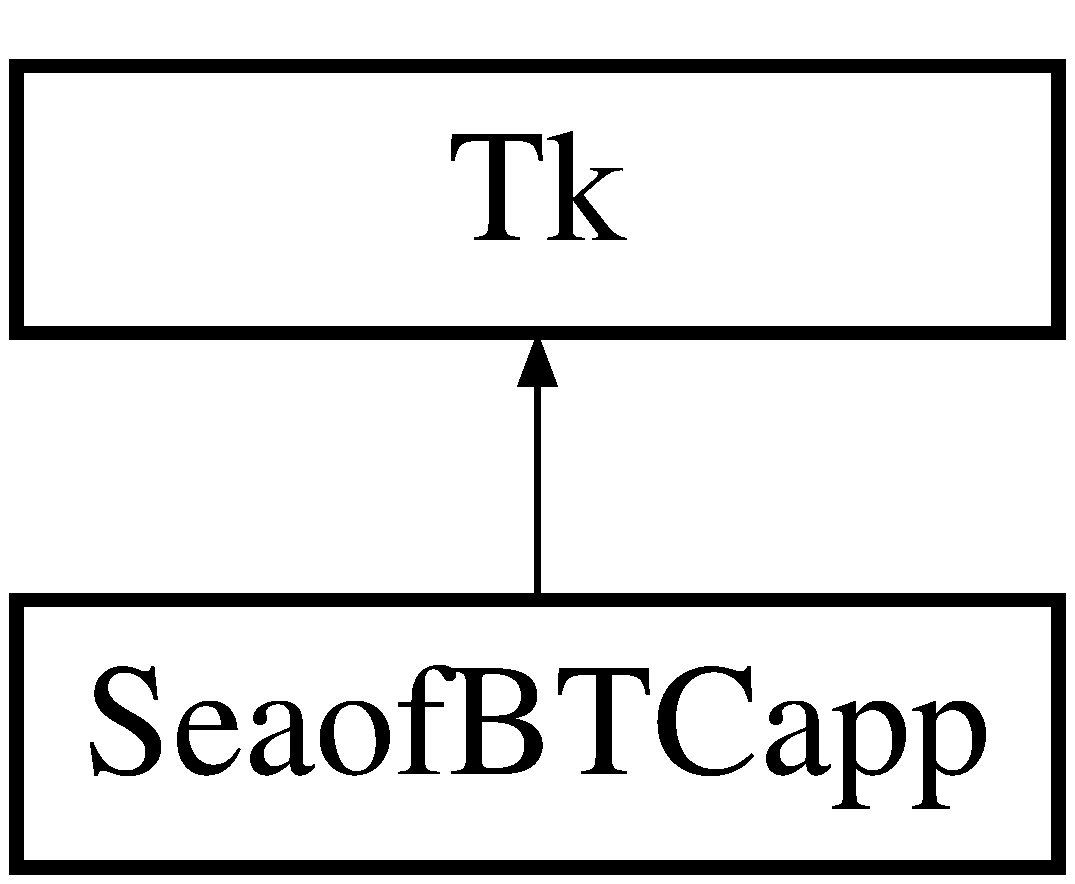
\includegraphics[height=2.000000cm]{class_test_menu_1_1_seaof_b_t_capp}
\end{center}
\end{figure}
\subsection*{Public Member Functions}
\begin{DoxyCompactItemize}
\item 
\mbox{\Hypertarget{class_test_menu_1_1_seaof_b_t_capp_a302afe6819b093163cc8ea6f029c75da}\label{class_test_menu_1_1_seaof_b_t_capp_a302afe6819b093163cc8ea6f029c75da}} 
def {\bfseries \+\_\+\+\_\+init\+\_\+\+\_\+} (self, args, kwargs)
\item 
\mbox{\Hypertarget{class_test_menu_1_1_seaof_b_t_capp_a590a388f6cd3c8fe0aa4ec4151c324a3}\label{class_test_menu_1_1_seaof_b_t_capp_a590a388f6cd3c8fe0aa4ec4151c324a3}} 
def {\bfseries show\+\_\+frame} (self, cont)
\end{DoxyCompactItemize}
\subsection*{Data Fields}
\begin{DoxyCompactItemize}
\item 
\mbox{\Hypertarget{class_test_menu_1_1_seaof_b_t_capp_a76a412a38642b618caf4a30f4cd2703c}\label{class_test_menu_1_1_seaof_b_t_capp_a76a412a38642b618caf4a30f4cd2703c}} 
{\bfseries frames}
\end{DoxyCompactItemize}


The documentation for this class was generated from the following file\+:\begin{DoxyCompactItemize}
\item 
C\+:/\+Users/pestourb/\+Documents/\+Git\+Hub/\+Secure\+Loc/Test\+Menu.\+py\end{DoxyCompactItemize}

\hypertarget{classsound_1_1_sound}{}\section{Sound Class Reference}
\label{classsound_1_1_sound}\index{Sound@{Sound}}
\subsection*{Public Member Functions}
\begin{DoxyCompactItemize}
\item 
\mbox{\Hypertarget{classsound_1_1_sound_ad296a3566bab38b1183e1c6644d24c26}\label{classsound_1_1_sound_ad296a3566bab38b1183e1c6644d24c26}} 
def {\bfseries \+\_\+\+\_\+init\+\_\+\+\_\+} (self, frequency, duration)
\item 
\mbox{\Hypertarget{classsound_1_1_sound_af1af6ddf04f00f958949618f79c33b82}\label{classsound_1_1_sound_af1af6ddf04f00f958949618f79c33b82}} 
def {\bfseries start} (self)
\item 
def \mbox{\hyperlink{classsound_1_1_sound_ad22709b2e67308af35f55680d5a026e0}{run}} (self)
\end{DoxyCompactItemize}
\subsection*{Data Fields}
\begin{DoxyCompactItemize}
\item 
\mbox{\Hypertarget{classsound_1_1_sound_abc7c2b8fc0432e1f1f6f07123a99a4a2}\label{classsound_1_1_sound_abc7c2b8fc0432e1f1f6f07123a99a4a2}} 
{\bfseries frequency}
\item 
\mbox{\Hypertarget{classsound_1_1_sound_a71f530f1f32dbca56a6af8a5fbbfbe49}\label{classsound_1_1_sound_a71f530f1f32dbca56a6af8a5fbbfbe49}} 
{\bfseries duration}
\end{DoxyCompactItemize}


\subsection{Detailed Description}
\begin{DoxyVerb}Allows generating customs sounds\end{DoxyVerb}
 

\subsection{Member Function Documentation}
\mbox{\Hypertarget{classsound_1_1_sound_ad22709b2e67308af35f55680d5a026e0}\label{classsound_1_1_sound_ad22709b2e67308af35f55680d5a026e0}} 
\index{sound\+::\+Sound@{sound\+::\+Sound}!run@{run}}
\index{run@{run}!sound\+::\+Sound@{sound\+::\+Sound}}
\subsubsection{\texorpdfstring{run()}{run()}}
{\footnotesize\ttfamily def run (\begin{DoxyParamCaption}\item[{}]{self }\end{DoxyParamCaption})}

\begin{DoxyVerb}plays the melody\end{DoxyVerb}
 

The documentation for this class was generated from the following file\+:\begin{DoxyCompactItemize}
\item 
C\+:/\+Users/pestourb/\+Documents/\+Git\+Hub/\+Secure\+Loc/sound.\+py\end{DoxyCompactItemize}

\hypertarget{class_test_menu_1_1_start_page}{}\section{Start\+Page Class Reference}
\label{class_test_menu_1_1_start_page}\index{Start\+Page@{Start\+Page}}
Inheritance diagram for Start\+Page\+:\begin{figure}[H]
\begin{center}
\leavevmode
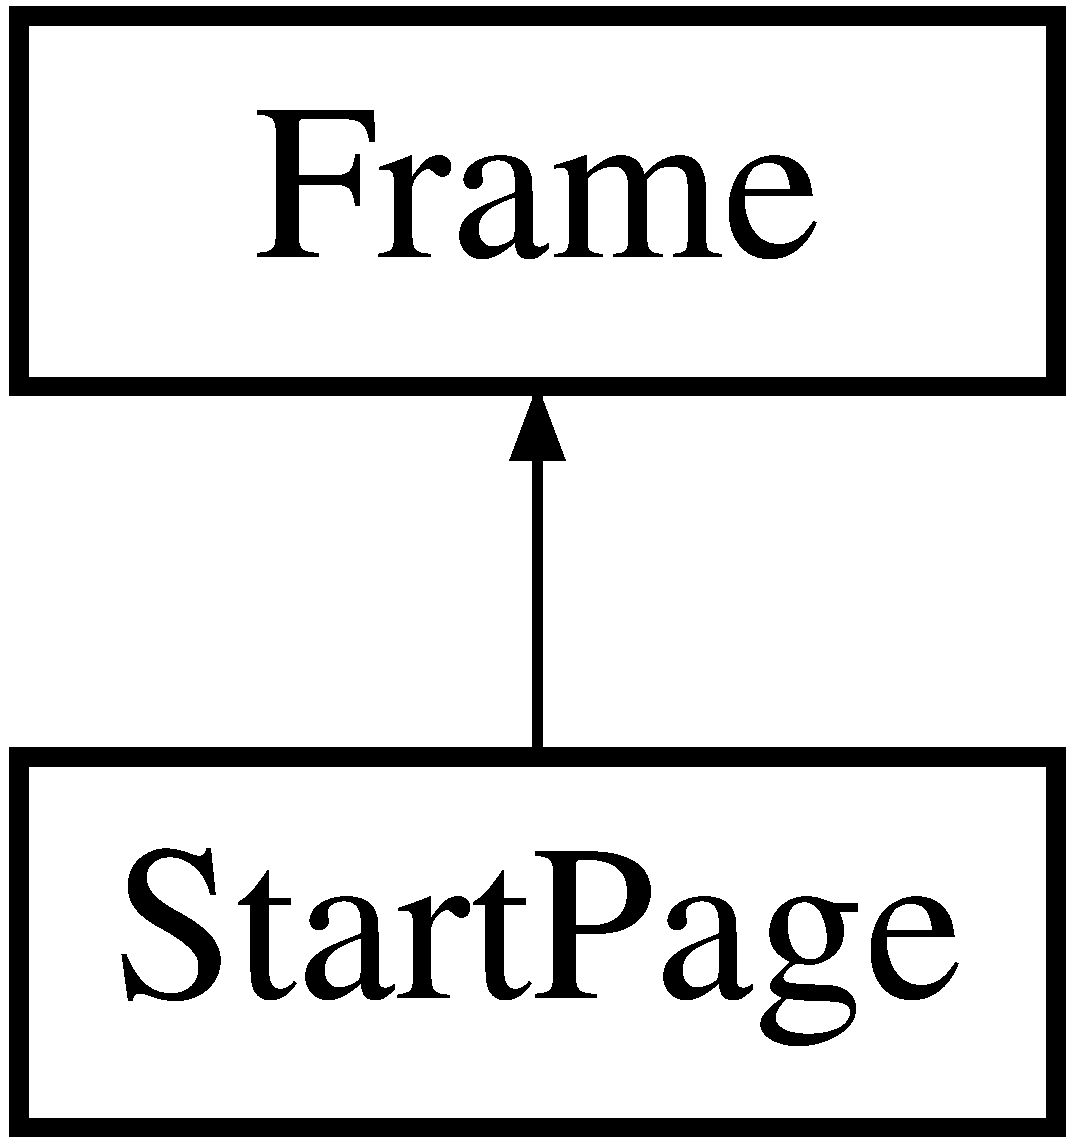
\includegraphics[height=2.000000cm]{class_test_menu_1_1_start_page}
\end{center}
\end{figure}
\subsection*{Public Member Functions}
\begin{DoxyCompactItemize}
\item 
\mbox{\Hypertarget{class_test_menu_1_1_start_page_a558d9afc290e8d1ff922f46114f16631}\label{class_test_menu_1_1_start_page_a558d9afc290e8d1ff922f46114f16631}} 
def {\bfseries \+\_\+\+\_\+init\+\_\+\+\_\+} (self, parent, controller)
\end{DoxyCompactItemize}


The documentation for this class was generated from the following file\+:\begin{DoxyCompactItemize}
\item 
C\+:/\+Users/pestourb/\+Documents/\+Git\+Hub/\+Secure\+Loc/Test\+Menu.\+py\end{DoxyCompactItemize}

\hypertarget{class_rendering_stub_1_1task}{}\section{task Class Reference}
\label{class_rendering_stub_1_1task}\index{task@{task}}
\subsection*{Public Member Functions}
\begin{DoxyCompactItemize}
\item 
\mbox{\Hypertarget{class_rendering_stub_1_1task_ae3242e112db05638dfbaf280c62891a0}\label{class_rendering_stub_1_1task_ae3242e112db05638dfbaf280c62891a0}} 
def {\bfseries \+\_\+\+\_\+init\+\_\+\+\_\+} (self, delay\+Time=0)
\end{DoxyCompactItemize}
\subsection*{Static Public Attributes}
\begin{DoxyCompactItemize}
\item 
\mbox{\Hypertarget{class_rendering_stub_1_1task_a5992b274cfdcacdbc1fa8347fd01ebde}\label{class_rendering_stub_1_1task_a5992b274cfdcacdbc1fa8347fd01ebde}} 
int {\bfseries done} = 0
\item 
\mbox{\Hypertarget{class_rendering_stub_1_1task_a961800bf60ff693820efbf7f4bc72788}\label{class_rendering_stub_1_1task_a961800bf60ff693820efbf7f4bc72788}} 
int {\bfseries cont} = 1
\item 
\mbox{\Hypertarget{class_rendering_stub_1_1task_aa5a4ff43956baf880d11d5af36d25674}\label{class_rendering_stub_1_1task_aa5a4ff43956baf880d11d5af36d25674}} 
int {\bfseries again} = 2
\end{DoxyCompactItemize}


\subsection{Detailed Description}
\begin{DoxyVerb}Stub for task class of Panda 3D\end{DoxyVerb}
 

The documentation for this class was generated from the following file\+:\begin{DoxyCompactItemize}
\item 
C\+:/\+Users/pestourb/\+Documents/\+Git\+Hub/\+Secure\+Loc/Rendering\+Stub.\+py\end{DoxyCompactItemize}

\hypertarget{class_rendering_stub_1_1task_mgr}{}\section{task\+Mgr Class Reference}
\label{class_rendering_stub_1_1task_mgr}\index{task\+Mgr@{task\+Mgr}}
Inheritance diagram for task\+Mgr\+:\begin{figure}[H]
\begin{center}
\leavevmode
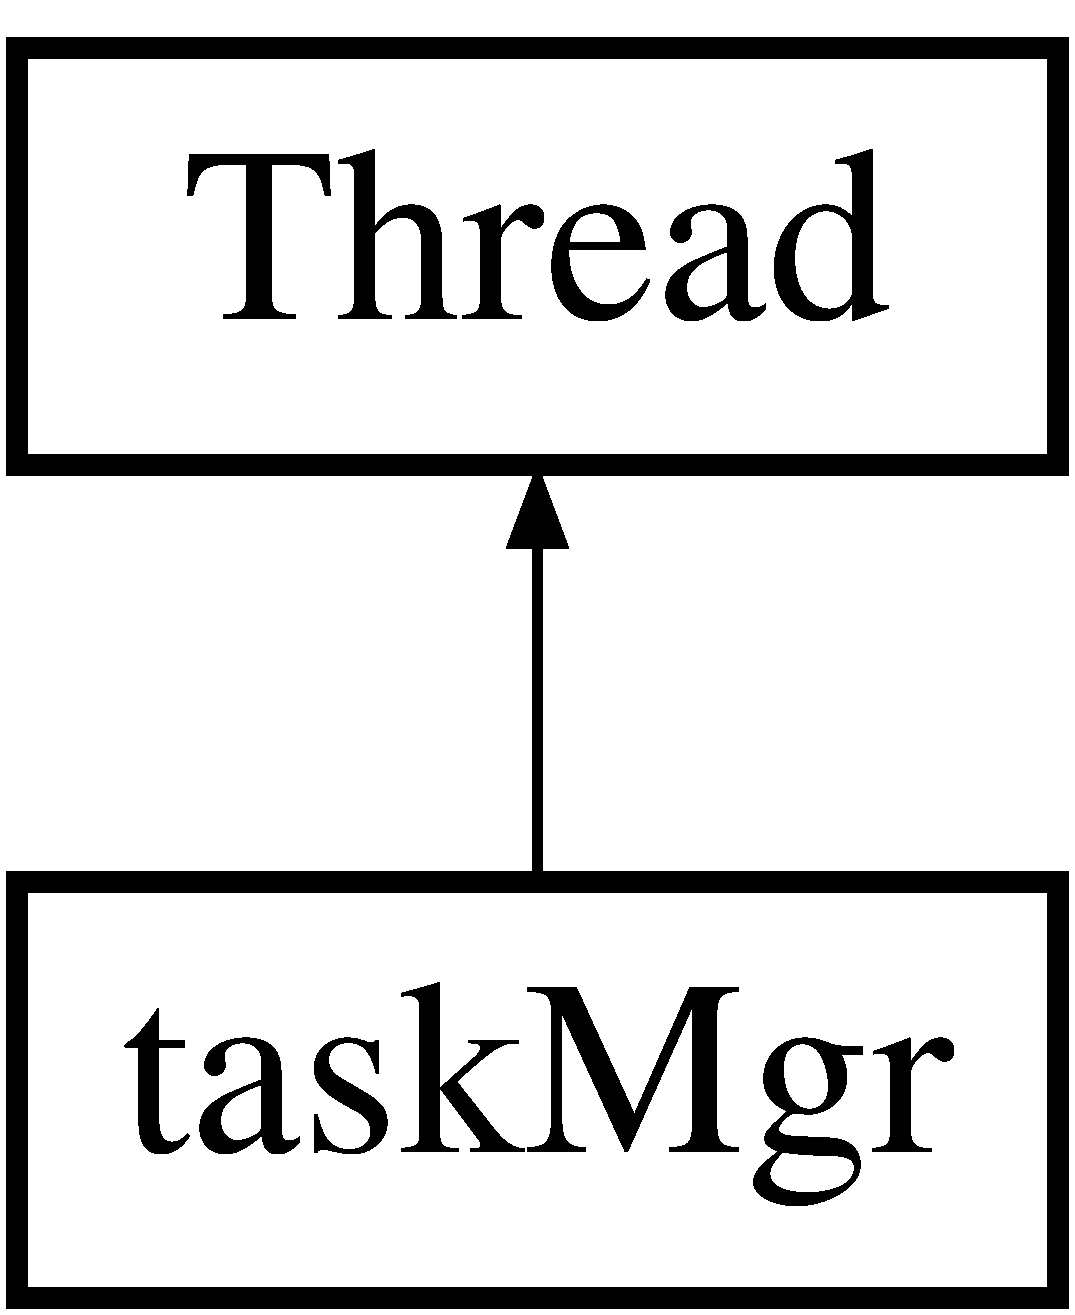
\includegraphics[height=2.000000cm]{class_rendering_stub_1_1task_mgr}
\end{center}
\end{figure}
\subsection*{Public Member Functions}
\begin{DoxyCompactItemize}
\item 
\mbox{\Hypertarget{class_rendering_stub_1_1task_mgr_acfc76021417da2e98b81ae907c817fa9}\label{class_rendering_stub_1_1task_mgr_acfc76021417da2e98b81ae907c817fa9}} 
def {\bfseries wrapper} (self, delay\+Time, target, name=\textquotesingle{}\textquotesingle{})
\item 
\mbox{\Hypertarget{class_rendering_stub_1_1task_mgr_a07fe9d7157eded83f29c5caa0e5f9148}\label{class_rendering_stub_1_1task_mgr_a07fe9d7157eded83f29c5caa0e5f9148}} 
def {\bfseries do\+Method\+Later} (self, delay\+Time, target, name=\textquotesingle{}\textquotesingle{})
\end{DoxyCompactItemize}


\subsection{Detailed Description}
\begin{DoxyVerb}Stub for Panda 3D taskMgr\end{DoxyVerb}
 

The documentation for this class was generated from the following file\+:\begin{DoxyCompactItemize}
\item 
C\+:/\+Users/pestourb/\+Documents/\+Git\+Hub/\+Secure\+Loc/Rendering\+Stub.\+py\end{DoxyCompactItemize}

\hypertarget{classworld_1_1_world}{}\section{World Class Reference}
\label{classworld_1_1_world}\index{World@{World}}
Inheritance diagram for World\+:\begin{figure}[H]
\begin{center}
\leavevmode
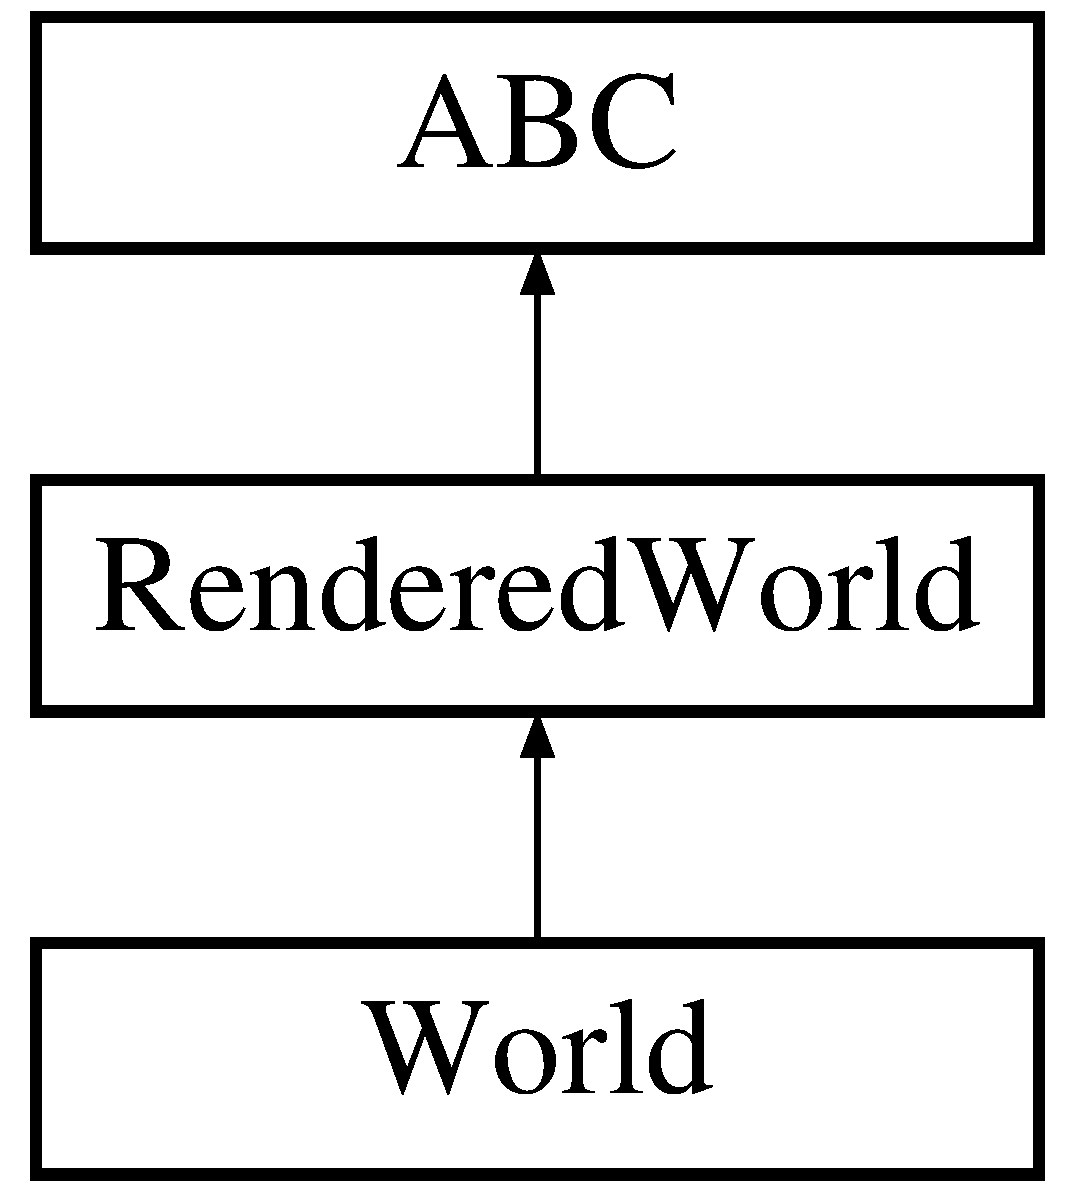
\includegraphics[height=3.000000cm]{classworld_1_1_world}
\end{center}
\end{figure}
\subsection*{Public Member Functions}
\begin{DoxyCompactItemize}
\item 
\mbox{\Hypertarget{classworld_1_1_world_ac775ee34451fdfa742b318538164070e}\label{classworld_1_1_world_ac775ee34451fdfa742b318538164070e}} 
def {\bfseries \+\_\+\+\_\+init\+\_\+\+\_\+}
\item 
def \mbox{\hyperlink{classworld_1_1_world_afc14fa698ef83ef5c8e17a2ee98d1375}{create\+\_\+anchors}} (self)
\item 
def \mbox{\hyperlink{classworld_1_1_world_a660f28d74c53fc654edf9e0d60c68d45}{gen\+\_\+anchors\+\_\+name}} (self, nb\+\_\+anchors)
\item 
def \mbox{\hyperlink{classworld_1_1_world_afdf01fd0b61dfe848a1606619c1b2902}{get\+\_\+target}} (self, robot)
\item 
\mbox{\Hypertarget{classworld_1_1_world_a55dd74ce9332b8fb3f6d5ff5dbd22aca}\label{classworld_1_1_world_a55dd74ce9332b8fb3f6d5ff5dbd22aca}} 
def {\bfseries update\+\_\+anchor}
\item 
\mbox{\Hypertarget{classworld_1_1_world_abfeee52c12f31bb94f7d6699303b515f}\label{classworld_1_1_world_abfeee52c12f31bb94f7d6699303b515f}} 
def {\bfseries ranging} (self, x, y, z, anchor\+\_\+idx)
\item 
def \mbox{\hyperlink{classworld_1_1_world_a04f4980a53d4b6e76ba5d02deb413780}{get\+\_\+distance}} (self, pos1, pos2)
\item 
def \mbox{\hyperlink{classworld_1_1_world_a5c63acf39eabba08715324da0d0ba2bd}{mse}} (self, rangings, pos)
\item 
def \mbox{\hyperlink{classworld_1_1_world_a9ee2b3e42f5d883afd028a9526c392d1}{gauss\+\_\+newton}} (self, rangings, start\+\_\+pos)
\item 
def \mbox{\hyperlink{classworld_1_1_world_a68d603f9d2b9759ddca06127f0899689}{iterate}} (self, rangings, start\+\_\+pos)
\item 
def \mbox{\hyperlink{classworld_1_1_world_a5b503b944cc95fd96a0e04f48e8c46fc}{localize}} (self, target)
\item 
def \mbox{\hyperlink{classworld_1_1_world_abd1ed1c4492cfa667fe9fda253df6173}{trilateration}} (self, target, anchor1, anchor2, anchor3=None, mode=\textquotesingle{}2\+D\textquotesingle{})
\item 
def \mbox{\hyperlink{classworld_1_1_world_a6886efcaba6a255c9d7566ba44f518f9}{update\+\_\+correction}} (self, rangings, solution)
\item 
def \mbox{\hyperlink{classworld_1_1_world_a34e56a6b0b7a51cc806cd0648a7ed275}{predict\+\_\+pos}} (self, robot)
\item 
def \mbox{\hyperlink{classworld_1_1_world_ad5a97b080a28cc5abda3903a686a56ff}{chose\+\_\+closest\+\_\+solution}} (self, solutions\+\_\+list, position)
\end{DoxyCompactItemize}
\subsection*{Data Fields}
\begin{DoxyCompactItemize}
\item 
\mbox{\Hypertarget{classworld_1_1_world_a5558ace5433f9aabbf0a0ec059900d94}\label{classworld_1_1_world_a5558ace5433f9aabbf0a0ec059900d94}} 
{\bfseries width}
\item 
\mbox{\Hypertarget{classworld_1_1_world_a509290c21d570ff479c1b9d9b1fe8810}\label{classworld_1_1_world_a509290c21d570ff479c1b9d9b1fe8810}} 
{\bfseries height}
\item 
\mbox{\Hypertarget{classworld_1_1_world_aba54450ad49ad1b46e29721241611d50}\label{classworld_1_1_world_aba54450ad49ad1b46e29721241611d50}} 
{\bfseries anchors}
\item 
\mbox{\Hypertarget{classworld_1_1_world_a5d2c023108742a1ce78ba9823c06ea35}\label{classworld_1_1_world_a5d2c023108742a1ce78ba9823c06ea35}} 
{\bfseries target}
\item 
\mbox{\Hypertarget{classworld_1_1_world_ac6c1eeb684483c821de0ec90f6c47cb9}\label{classworld_1_1_world_ac6c1eeb684483c821de0ec90f6c47cb9}} 
{\bfseries shown}
\end{DoxyCompactItemize}


\subsection{Detailed Description}
\begin{DoxyVerb}World class, represents the room in which the robots will evolve.
The world contains the anchors with their positions, and is able
to return the positions of the robots or whatever is moving in it\end{DoxyVerb}
 

\subsection{Member Function Documentation}
\mbox{\Hypertarget{classworld_1_1_world_ad5a97b080a28cc5abda3903a686a56ff}\label{classworld_1_1_world_ad5a97b080a28cc5abda3903a686a56ff}} 
\index{world\+::\+World@{world\+::\+World}!chose\+\_\+closest\+\_\+solution@{chose\+\_\+closest\+\_\+solution}}
\index{chose\+\_\+closest\+\_\+solution@{chose\+\_\+closest\+\_\+solution}!world\+::\+World@{world\+::\+World}}
\subsubsection{\texorpdfstring{chose\+\_\+closest\+\_\+solution()}{chose\_closest\_solution()}}
{\footnotesize\ttfamily def chose\+\_\+closest\+\_\+solution (\begin{DoxyParamCaption}\item[{}]{self,  }\item[{}]{solutions\+\_\+list,  }\item[{}]{position }\end{DoxyParamCaption})}

\begin{DoxyVerb}returns the closest solution of solutions_list from the given position\end{DoxyVerb}
 \mbox{\Hypertarget{classworld_1_1_world_afc14fa698ef83ef5c8e17a2ee98d1375}\label{classworld_1_1_world_afc14fa698ef83ef5c8e17a2ee98d1375}} 
\index{world\+::\+World@{world\+::\+World}!create\+\_\+anchors@{create\+\_\+anchors}}
\index{create\+\_\+anchors@{create\+\_\+anchors}!world\+::\+World@{world\+::\+World}}
\subsubsection{\texorpdfstring{create\+\_\+anchors()}{create\_anchors()}}
{\footnotesize\ttfamily def create\+\_\+anchors (\begin{DoxyParamCaption}\item[{}]{self }\end{DoxyParamCaption})}

\begin{DoxyVerb}Displays anchors\end{DoxyVerb}
 \mbox{\Hypertarget{classworld_1_1_world_a9ee2b3e42f5d883afd028a9526c392d1}\label{classworld_1_1_world_a9ee2b3e42f5d883afd028a9526c392d1}} 
\index{world\+::\+World@{world\+::\+World}!gauss\+\_\+newton@{gauss\+\_\+newton}}
\index{gauss\+\_\+newton@{gauss\+\_\+newton}!world\+::\+World@{world\+::\+World}}
\subsubsection{\texorpdfstring{gauss\+\_\+newton()}{gauss\_newton()}}
{\footnotesize\ttfamily def gauss\+\_\+newton (\begin{DoxyParamCaption}\item[{}]{self,  }\item[{}]{rangings,  }\item[{}]{start\+\_\+pos }\end{DoxyParamCaption})}

\begin{DoxyVerb}applies Gauss-Newton on the set of rangings to find the tag's position. Uses the given position as starting point\end{DoxyVerb}
 \mbox{\Hypertarget{classworld_1_1_world_a660f28d74c53fc654edf9e0d60c68d45}\label{classworld_1_1_world_a660f28d74c53fc654edf9e0d60c68d45}} 
\index{world\+::\+World@{world\+::\+World}!gen\+\_\+anchors\+\_\+name@{gen\+\_\+anchors\+\_\+name}}
\index{gen\+\_\+anchors\+\_\+name@{gen\+\_\+anchors\+\_\+name}!world\+::\+World@{world\+::\+World}}
\subsubsection{\texorpdfstring{gen\+\_\+anchors\+\_\+name()}{gen\_anchors\_name()}}
{\footnotesize\ttfamily def gen\+\_\+anchors\+\_\+name (\begin{DoxyParamCaption}\item[{}]{self,  }\item[{}]{nb\+\_\+anchors }\end{DoxyParamCaption})}

\begin{DoxyVerb}generates a list of anchors id for the given total number of anchors\end{DoxyVerb}
 \mbox{\Hypertarget{classworld_1_1_world_a04f4980a53d4b6e76ba5d02deb413780}\label{classworld_1_1_world_a04f4980a53d4b6e76ba5d02deb413780}} 
\index{world\+::\+World@{world\+::\+World}!get\+\_\+distance@{get\+\_\+distance}}
\index{get\+\_\+distance@{get\+\_\+distance}!world\+::\+World@{world\+::\+World}}
\subsubsection{\texorpdfstring{get\+\_\+distance()}{get\_distance()}}
{\footnotesize\ttfamily def get\+\_\+distance (\begin{DoxyParamCaption}\item[{}]{self,  }\item[{}]{pos1,  }\item[{}]{pos2 }\end{DoxyParamCaption})}

\begin{DoxyVerb}returns the distance between pos1 and pos2\end{DoxyVerb}
 \mbox{\Hypertarget{classworld_1_1_world_afdf01fd0b61dfe848a1606619c1b2902}\label{classworld_1_1_world_afdf01fd0b61dfe848a1606619c1b2902}} 
\index{world\+::\+World@{world\+::\+World}!get\+\_\+target@{get\+\_\+target}}
\index{get\+\_\+target@{get\+\_\+target}!world\+::\+World@{world\+::\+World}}
\subsubsection{\texorpdfstring{get\+\_\+target()}{get\_target()}}
{\footnotesize\ttfamily def get\+\_\+target (\begin{DoxyParamCaption}\item[{}]{self,  }\item[{}]{robot }\end{DoxyParamCaption})}

\begin{DoxyVerb}gets the id of the robot to localize\end{DoxyVerb}
 \mbox{\Hypertarget{classworld_1_1_world_a68d603f9d2b9759ddca06127f0899689}\label{classworld_1_1_world_a68d603f9d2b9759ddca06127f0899689}} 
\index{world\+::\+World@{world\+::\+World}!iterate@{iterate}}
\index{iterate@{iterate}!world\+::\+World@{world\+::\+World}}
\subsubsection{\texorpdfstring{iterate()}{iterate()}}
{\footnotesize\ttfamily def iterate (\begin{DoxyParamCaption}\item[{}]{self,  }\item[{}]{rangings,  }\item[{}]{start\+\_\+pos }\end{DoxyParamCaption})}

\begin{DoxyVerb}Finds the minimum MSE in the neighborhood of start_pos and repeats the process from that new position\end{DoxyVerb}
 \mbox{\Hypertarget{classworld_1_1_world_a5b503b944cc95fd96a0e04f48e8c46fc}\label{classworld_1_1_world_a5b503b944cc95fd96a0e04f48e8c46fc}} 
\index{world\+::\+World@{world\+::\+World}!localize@{localize}}
\index{localize@{localize}!world\+::\+World@{world\+::\+World}}
\subsubsection{\texorpdfstring{localize()}{localize()}}
{\footnotesize\ttfamily def localize (\begin{DoxyParamCaption}\item[{}]{self,  }\item[{}]{target }\end{DoxyParamCaption})}

\begin{DoxyVerb}localizes the given target\end{DoxyVerb}
 \mbox{\Hypertarget{classworld_1_1_world_a5c63acf39eabba08715324da0d0ba2bd}\label{classworld_1_1_world_a5c63acf39eabba08715324da0d0ba2bd}} 
\index{world\+::\+World@{world\+::\+World}!mse@{mse}}
\index{mse@{mse}!world\+::\+World@{world\+::\+World}}
\subsubsection{\texorpdfstring{mse()}{mse()}}
{\footnotesize\ttfamily def mse (\begin{DoxyParamCaption}\item[{}]{self,  }\item[{}]{rangings,  }\item[{}]{pos }\end{DoxyParamCaption})}

\begin{DoxyVerb}Calculates the Mean Square Error of the given position.
Error is defined as the difference between the ranging of the given position and the given rangings\end{DoxyVerb}
 \mbox{\Hypertarget{classworld_1_1_world_a34e56a6b0b7a51cc806cd0648a7ed275}\label{classworld_1_1_world_a34e56a6b0b7a51cc806cd0648a7ed275}} 
\index{world\+::\+World@{world\+::\+World}!predict\+\_\+pos@{predict\+\_\+pos}}
\index{predict\+\_\+pos@{predict\+\_\+pos}!world\+::\+World@{world\+::\+World}}
\subsubsection{\texorpdfstring{predict\+\_\+pos()}{predict\_pos()}}
{\footnotesize\ttfamily def predict\+\_\+pos (\begin{DoxyParamCaption}\item[{}]{self,  }\item[{}]{robot }\end{DoxyParamCaption})}

\begin{DoxyVerb}estimates the position at the next iteration based on tag's speed\end{DoxyVerb}
 \mbox{\Hypertarget{classworld_1_1_world_abd1ed1c4492cfa667fe9fda253df6173}\label{classworld_1_1_world_abd1ed1c4492cfa667fe9fda253df6173}} 
\index{world\+::\+World@{world\+::\+World}!trilateration@{trilateration}}
\index{trilateration@{trilateration}!world\+::\+World@{world\+::\+World}}
\subsubsection{\texorpdfstring{trilateration()}{trilateration()}}
{\footnotesize\ttfamily def trilateration (\begin{DoxyParamCaption}\item[{}]{self,  }\item[{}]{target,  }\item[{}]{anchor1,  }\item[{}]{anchor2,  }\item[{}]{anchor3 = {\ttfamily None},  }\item[{}]{mode = {\ttfamily \textquotesingle{}2D\textquotesingle{}} }\end{DoxyParamCaption})}

\begin{DoxyVerb}computes the trilateration of target based on the rangings from anchor 1 and 2.
Two solutions are obtained based on Pythagora's theorem, both are returned\end{DoxyVerb}
 \mbox{\Hypertarget{classworld_1_1_world_a6886efcaba6a255c9d7566ba44f518f9}\label{classworld_1_1_world_a6886efcaba6a255c9d7566ba44f518f9}} 
\index{world\+::\+World@{world\+::\+World}!update\+\_\+correction@{update\+\_\+correction}}
\index{update\+\_\+correction@{update\+\_\+correction}!world\+::\+World@{world\+::\+World}}
\subsubsection{\texorpdfstring{update\+\_\+correction()}{update\_correction()}}
{\footnotesize\ttfamily def update\+\_\+correction (\begin{DoxyParamCaption}\item[{}]{self,  }\item[{}]{rangings,  }\item[{}]{solution }\end{DoxyParamCaption})}

\begin{DoxyVerb}dynamically corrects the offset applied to the rangings, by comparing the received ranging value to the estimated one.
    The correction is based on a ratio of the difference between the two values\end{DoxyVerb}
 

The documentation for this class was generated from the following file\+:\begin{DoxyCompactItemize}
\item 
C\+:/\+Users/pestourb/\+Documents/\+Git\+Hub/\+Secure\+Loc/world.\+py\end{DoxyCompactItemize}

%--- End generated contents ---

% Index
\backmatter
\newpage
\phantomsection
\clearemptydoublepage
\addcontentsline{toc}{chapter}{Index}
\printindex

\end{document}
